\documentclass[11pt,]{isuthesis}
\usepackage{lmodern}

\usepackage{isutraditional}
\chaptertitle
\alternate

\usepackage{amssymb,amsmath,mathptmx,stmaryrd}
\usepackage{ifxetex,ifluatex}
\usepackage{fixltx2e} % provides \textsubscript
\ifnum 0\ifxetex 1\fi\ifluatex 1\fi=0 % if pdftex
  \usepackage[T1]{fontenc}
  \usepackage[utf8]{inputenc}
\else % if luatex or xelatex
  \ifxetex
    \usepackage{mathspec}
  \else
    \usepackage{fontspec}
  \fi
  \defaultfontfeatures{Ligatures=TeX,Scale=MatchLowercase}
\fi
% use upquote if available, for straight quotes in verbatim environments
\IfFileExists{upquote.sty}{\usepackage{upquote}}{}
% use microtype if available
\IfFileExists{microtype.sty}{%
\usepackage{microtype}
\UseMicrotypeSet[protrusion]{basicmath} % disable protrusion for tt fonts
}{}

\usepackage{natbib}
\bibliographystyle{apa}


% http://tex.stackexchange.com/questions/3033/forcing-linebreaks-in-url
\PassOptionsToPackage{hyphens}{url}\usepackage{hyperref}
\PassOptionsToPackage{usenames,dvipsnames}{color} % color is loaded by hyperref
\hypersetup{unicode=true,
            pdftitle={A Cartridge Case Comparison Pipeline},
            pdfauthor={Joseph Zemmels},
            colorlinks=true,
            linkcolor=Black,
            citecolor=Black,
            urlcolor=blue,
            breaklinks=true}
\urlstyle{same}  % don't use monospace font for urls

\usepackage{color}
\usepackage{fancyvrb}
\newcommand{\VerbBar}{|}
\newcommand{\VERB}{\Verb[commandchars=\\\{\}]}
\DefineVerbatimEnvironment{Highlighting}{Verbatim}{commandchars=\\\{\}}
% Add ',fontsize=\small' for more characters per line
\usepackage{framed}
\definecolor{shadecolor}{RGB}{248,248,248}
\newenvironment{Shaded}{\begin{snugshade}}{\end{snugshade}}
\newcommand{\AlertTok}[1]{\textcolor[rgb]{0.94,0.16,0.16}{#1}}
\newcommand{\AnnotationTok}[1]{\textcolor[rgb]{0.56,0.35,0.01}{\textbf{\textit{#1}}}}
\newcommand{\AttributeTok}[1]{\textcolor[rgb]{0.77,0.63,0.00}{#1}}
\newcommand{\BaseNTok}[1]{\textcolor[rgb]{0.00,0.00,0.81}{#1}}
\newcommand{\BuiltInTok}[1]{#1}
\newcommand{\CharTok}[1]{\textcolor[rgb]{0.31,0.60,0.02}{#1}}
\newcommand{\CommentTok}[1]{\textcolor[rgb]{0.56,0.35,0.01}{\textit{#1}}}
\newcommand{\CommentVarTok}[1]{\textcolor[rgb]{0.56,0.35,0.01}{\textbf{\textit{#1}}}}
\newcommand{\ConstantTok}[1]{\textcolor[rgb]{0.00,0.00,0.00}{#1}}
\newcommand{\ControlFlowTok}[1]{\textcolor[rgb]{0.13,0.29,0.53}{\textbf{#1}}}
\newcommand{\DataTypeTok}[1]{\textcolor[rgb]{0.13,0.29,0.53}{#1}}
\newcommand{\DecValTok}[1]{\textcolor[rgb]{0.00,0.00,0.81}{#1}}
\newcommand{\DocumentationTok}[1]{\textcolor[rgb]{0.56,0.35,0.01}{\textbf{\textit{#1}}}}
\newcommand{\ErrorTok}[1]{\textcolor[rgb]{0.64,0.00,0.00}{\textbf{#1}}}
\newcommand{\ExtensionTok}[1]{#1}
\newcommand{\FloatTok}[1]{\textcolor[rgb]{0.00,0.00,0.81}{#1}}
\newcommand{\FunctionTok}[1]{\textcolor[rgb]{0.00,0.00,0.00}{#1}}
\newcommand{\ImportTok}[1]{#1}
\newcommand{\InformationTok}[1]{\textcolor[rgb]{0.56,0.35,0.01}{\textbf{\textit{#1}}}}
\newcommand{\KeywordTok}[1]{\textcolor[rgb]{0.13,0.29,0.53}{\textbf{#1}}}
\newcommand{\NormalTok}[1]{#1}
\newcommand{\OperatorTok}[1]{\textcolor[rgb]{0.81,0.36,0.00}{\textbf{#1}}}
\newcommand{\OtherTok}[1]{\textcolor[rgb]{0.56,0.35,0.01}{#1}}
\newcommand{\PreprocessorTok}[1]{\textcolor[rgb]{0.56,0.35,0.01}{\textit{#1}}}
\newcommand{\RegionMarkerTok}[1]{#1}
\newcommand{\SpecialCharTok}[1]{\textcolor[rgb]{0.00,0.00,0.00}{#1}}
\newcommand{\SpecialStringTok}[1]{\textcolor[rgb]{0.31,0.60,0.02}{#1}}
\newcommand{\StringTok}[1]{\textcolor[rgb]{0.31,0.60,0.02}{#1}}
\newcommand{\VariableTok}[1]{\textcolor[rgb]{0.00,0.00,0.00}{#1}}
\newcommand{\VerbatimStringTok}[1]{\textcolor[rgb]{0.31,0.60,0.02}{#1}}
\newcommand{\WarningTok}[1]{\textcolor[rgb]{0.56,0.35,0.01}{\textbf{\textit{#1}}}}
\usepackage{longtable,booktabs,widetable}

% always, graphics silly
\usepackage{graphicx,grffile}
\makeatletter
\def\maxwidth{\ifdim\Gin@nat@width>\linewidth\linewidth\else\Gin@nat@width\fi}
\def\maxheight{\ifdim\Gin@nat@height>\textheight\textheight\else\Gin@nat@height\fi}
\makeatother
% Scale images if necessary, so that they will not overflow the page
% margins by default, and it is still possible to overwrite the defaults
% using explicit options in \includegraphics[width, height, ...]{}
\setkeys{Gin}{width=\maxwidth,height=\maxheight,keepaspectratio}

%%%%%%%%%%%%%%%%%%%%%%%%%%%%%%%%%%%%%%%%%%%%%%%%%%%%
% Taken from bookdown preamble
%%%%%%%%%%%%%%%%%%%%%%%%%%%%%%%%%%%%%%%%%%%%%%%%%%%%

\usepackage{booktabs}
\usepackage{longtable}
\usepackage{framed,color}
\definecolor{shadecolor}{RGB}{248,248,248}

\ifxetex
  \usepackage{letltxmacro}
  \setlength{\XeTeXLinkMargin}{1pt}
  \LetLtxMacro\SavedIncludeGraphics\includegraphics
  \def\includegraphics#1#{% #1 catches optional stuff (star/opt. arg.)
    \IncludeGraphicsAux{#1}%
  }%
  \newcommand*{\IncludeGraphicsAux}[2]{%
    \XeTeXLinkBox{%
      \SavedIncludeGraphics#1{#2}%
    }%
  }%
\fi

\newenvironment{rmdblock}[1]
  {\begin{shaded*}
  \begin{itemize}
  \renewcommand{\labelitemi}{
    \raisebox{-.7\height}[0pt][0pt]{
      {\setkeys{Gin}{width=3em,keepaspectratio}\includegraphics{images/#1}}
    }
  }
  \item
  }
  {
  \end{itemize}
  \end{shaded*}
  }
\newenvironment{rmdnote}
  {\begin{rmdblock}{note}}
  {\end{rmdblock}}
\newenvironment{rmdcaution}
  {\begin{rmdblock}{caution}}
  {\end{rmdblock}}
\newenvironment{rmdimportant}
  {\begin{rmdblock}{important}}
  {\end{rmdblock}}
\newenvironment{rmdtip}
  {\begin{rmdblock}{tip}}
  {\end{rmdblock}}
\newenvironment{rmdwarning}
  {\begin{rmdblock}{warning}}
  {\end{rmdblock}}

%%%%%%%%%%%%%%%%%%%%%%%%%%%%%%%%%%%%%%%%%%%%%%%%%%%%
% Taken from bookdown preamble
%%%%%%%%%%%%%%%%%%%%%%%%%%%%%%%%%%%%%%%%%%%%%%%%%%%%


\IfFileExists{parskip.sty}{%
\usepackage{parskip}
}{% else
\setlength{\parindent}{0pt}
\setlength{\parskip}{6pt plus 2pt minus 1pt}
}
\setlength{\emergencystretch}{3em}  % prevent overfull lines
\providecommand{\tightlist}{%
  \setlength{\itemsep}{0pt}\setlength{\parskip}{0pt}}
\setcounter{secnumdepth}{5}
% Redefines (sub)paragraphs to behave more like sections
\ifx\paragraph\undefined\else
\let\oldparagraph\paragraph
\renewcommand{\paragraph}[1]{\oldparagraph{#1}\mbox{}}
\fi
\ifx\subparagraph\undefined\else
\let\oldsubparagraph\subparagraph
\renewcommand{\subparagraph}[1]{\oldsubparagraph{#1}\mbox{}}
\fi

%%% Use protect on footnotes to avoid problems with footnotes in titles
\let\rmarkdownfootnote\footnote%
\def\footnote{\protect\rmarkdownfootnote}

%%% Change title format to be more compact
%\usepackage{titling}

% Create subtitle command for use in maketitle
\newcommand{\subtitle}[1]{
 \posttitle{
   \begin{center}\large#1\end{center}
   }
}

%\setlength{\droptitle}{-2em}
 \title{A Cartridge Case Comparison Pipeline}
 \author{Joseph Zemmels}
 \date{}
\degree{DOCTOR OF PHILOSOPHY}
\major{Statistics}
\mprof{Heike Hofmann}
\members{Alicia Carriquiry \\ Kori Khan \\ Danica Ommen \\ Richard Stone \\ Susan VanderPlas}

\usepackage{booktabs}
\usepackage{longtable}
\usepackage{array}
\usepackage{multirow}
\usepackage{wrapfig}
\usepackage{float}
\usepackage{colortbl}
\usepackage{pdflscape}
\usepackage{tabu}
\usepackage{threeparttable}
\usepackage{threeparttablex}
\usepackage[normalem]{ulem}
\usepackage{makecell}
\usepackage{xcolor}

\widowpenalty10000
\clubpenalty10000
%\raggedbottom


%%%%%%%
%% Hacks
\usepackage{environ}

\NewEnviron{paperinfo_}{%
  \paperinfo{\BODY}
  }

\NewEnviron{paperauthor_}{%
  \paperauthor{\BODY}
  }

\let\oldappendix\appendix
\renewcommand{\appendix}{
\appendixtitle
\oldappendix
}
%%%%%%%

\begin{document}

\maketitle


% Optional thesis dedication
\cleardoublepage \phantomsection
\chapter*{DEDICATION}

For Emily.

{
\hypersetup{linkcolor=black}
\vspace{-2cm}
\setcounter{tocdepth}{2}
\tableofcontents
}

\addtocontents{toc}{\def\protect\@chapapp{}}
\cleardoublepage \phantomsection \addcontentsline{toc}{chapter}{LIST OF TABLES}
\listoftables
\cleardoublepage \phantomsection \addcontentsline{toc}{chapter}{LIST OF FIGURES}
\listoffigures

\addtocontents{toc}{\def\protect\@chapapp{CHAPTER\ }}

\cleardoublepage \phantomsection
\specialchapt{ACKNOWLEDGEMENTS}

This work was partially funded by the Center for Statistics and Applications in Forensic Evidence (CSAFE) through Cooperative Agreement 70NANB20H019 between NIST and Iowa State University, which includes activities carried out at Carnegie Mellon University, Duke University, University of California Irvine, University of Virginia, West Virginia University, University of Pennsylvania, Swarthmore College and University of Nebraska, Lincoln.


%\addtocontents{toc}{\def\protect\@chapapp{CHAPTER\ }}

\specialchapt{ABSTRACT}
Algorithms to compare evidence are increasingly used in forensic examinations to supplement an examiner's opinion with an objective measure of similarity. However, an algorithm must first be thoroughly tested under various conditions to identify its strengths and weaknesses. This experimentation is expedited for algorithms that are accessible to fellow researchers and practitioners. In this work, we discuss an algorithm to objectively measure the similarity between cartridge cases. We have designed this algorithm to be approachable for researchers and practitioners alike. Chapter 2 discusses a modularization of the algorithm into a ``pipeline'' that enables reproducibility, experimentation, and comprehension. Our goal in this modularization is to lay a foundation upon which improvements can be easily developed. Chapter 3 details a suite of diagnostic tools that illuminate the inner-workings of the algorithm and determine when and why the algorithm ``works'' correctly. These diagnostics will be useful for both researchers interested in correcting the algorithm's behavior and for practitioners concerned with applying the algorithm to case work. Chapter 4 introduces novel pieces of the pipeline that we demonstrate are improvements to predominant methods. In particular, we introduce the Automatic Cartridge Evidence Scoring (ACES) algorithm that measures the similarity between two cartridge cases using a novel set of numeric features.

\newpage
\pagenumbering{arabic}

\setlength\parindent{24pt}

\hypertarget{literature-review}{%
\chapter{Literature Review}\label{literature-review}}

\hypertarget{preliminaries-forensic-examinations}{%
\section{Preliminaries: Forensic Examinations}\label{preliminaries-forensic-examinations}}

A bullet casing is found at the scene of a murder.
The bullet is recovered from the victim during autopsy.
A handwritten letter threatening the victim is found in their pocket.
The assailant's shoeprints are discovered fleeing the area.
Who left this evidence?
Investigators obtain the gun, shoes, and handwriting samples of a suspect.
This evidence, along with the crime scene evidence, is sent to a forensic laboratory for analysis.
Forensic examiners compare the evidence to establish whether they share a common source.
The suspect is charged after the examiners conclude that there is sufficient agreement between the crime scene and suspect's samples.

The procedure described above, in which evidence is analyzed to determine its origin, is called the \emph{source identification} problem \citep{Ommen2018}.
Historically, forensic examiners have relied on tools (e.g., microscopes), case facts, and experience to develop an opinion on the similarity of two pieces of evidence.
More recently, algorithms to automatically compare evidence and provide an objective measure of similarity have been introduced.
These algorithms can be used in a forensic examination to supplement and inform the examiner's conclusion.
We propose an automatic, objective solution to the source identification problem; specifically in the context of comparing fired \emph{cartridge cases.}
Cartridge case comparison is a sub-discipline of Firearm and Toolmark Identification, which is reviewed in the next section.

\hypertarget{firearm-and-toolmark-identification}{%
\subsection{Firearm and Toolmark Identification}\label{firearm-and-toolmark-identification}}

Firearm and toolmark identification involves studying markings or impressions left by a hard surface such as a firearm or screwdriver on a softer surface \citep{Thompson2017}.
For example, a barrel's rifling leaves toolmarks on a bullet as it travels out of the gun.

\hypertarget{the-firing-process}{%
\subsubsection{The Firing Process}\label{the-firing-process}}

In this section, we describe the basic process of firing a cartridge out of a handgun or rifle.
A \emph{cartridge} consists of a metal casing containing primer, gunpowder, and a bullet.
Figure \ref{fig:cartridgeDiagram} shows a cross-section of a cartridge featuring these components \citep{calibersExplained}.

\begin{figure}[!htbp]

{\centering 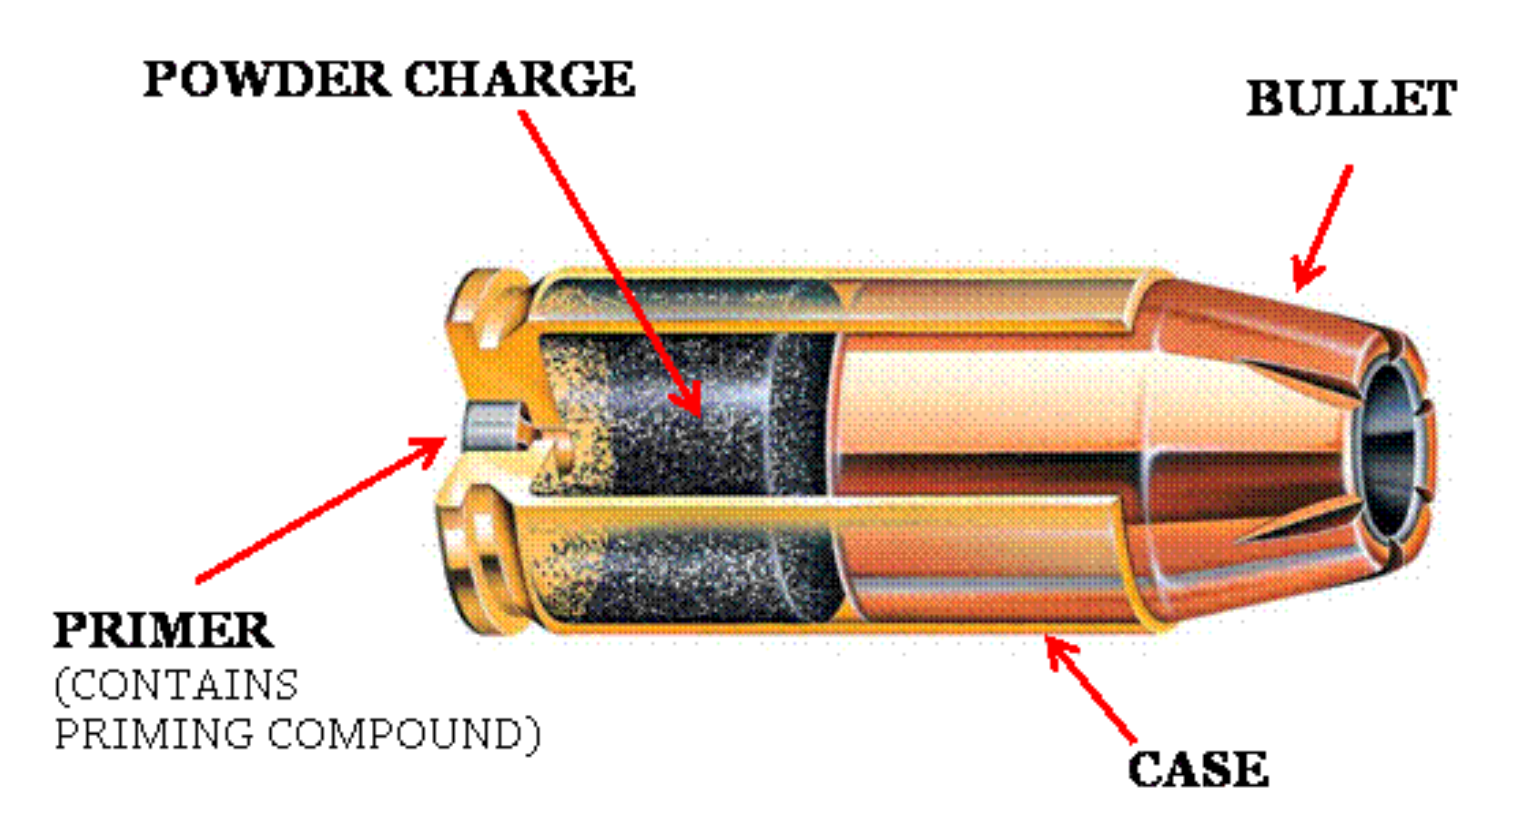
\includegraphics[width=.5\textwidth]{images/bulletdiagram1} 

}

\caption{A cartridge containing primer, powder, and a bullet. The firing process is initiated by loading a cartridge into the barrel of a firearm.}\label{fig:cartridgeDiagram}
\end{figure}

First, a cartridge is loaded into the back of the barrel in an area called the \emph{chamber}.
Figure \ref{fig:pistolParts} shows an example of a cartridge loaded into the chamber of a pistol \citep{rattenbury}.
Note that the hammer of the pistol in Figure \ref{fig:pistolParts} is pulled to hold the firing pin under spring tension.
Upon squeezing the trigger, the firing pin releases and travels forwards at a high velocity.
The firing pin strikes the primer of the cartridge case, causing it to explode.

\begin{figure}[!htbp]

{\centering 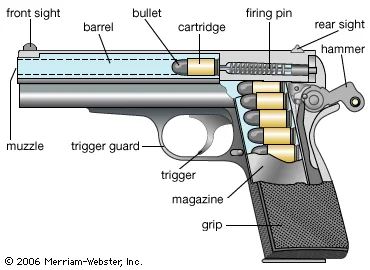
\includegraphics[width=.5\textwidth]{images/Parts-pistol} 

}

\caption{Cross-section of a pistol with a chambered cartridge and drawn-back hammer. Pulling the trigger releases the firing pin which strikes the cartridge case primer.}\label{fig:pistolParts}
\end{figure}

The explosion of the primer ignites the powder in the cartridge \citep{hampton}.
As shown in \ref{fig:firingCartridge}, gas rapidly expands in the cartridge that pushes the bullet down the barrel.
Simultaneously, the rest of the cartridge travels towards the back of the barrel and strikes the back wall of the barrel, known as the \emph{breech face}, with considerable force.

\begin{figure}[!htbp]

{\centering 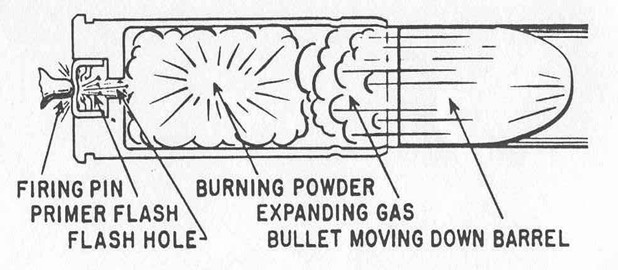
\includegraphics[width=.5\textwidth]{images/firingCartridgeDiagram} 

}

\caption{A cartridge after a firing pin has struck the primer. The explosion of the primer ignites the powder within the cartridge, causing gas to rapidly expand and force the bullet down the barrel.}\label{fig:firingCartridge}
\end{figure}

Any markings on the breech face are imprinted onto the cartridge case, creating the so-called \emph{breech face impressions}.
These impressions are analogous to a barrel's ``fingerprint'' left on the cartridge case.
Figure \ref{fig:impressionDiagram} shows cartoon examples of breech face markings that appear on cartridge cases \citep{hampton}.

\begin{figure}[!htbp]

{\centering 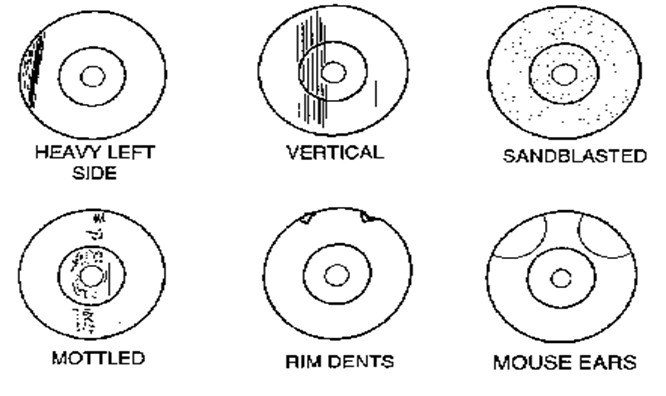
\includegraphics[width=.5\textwidth]{images/breechFaceImpressionDiagram} 

}

\caption{Examples of common breech face impression patterns. These are considered analogous to a breech face fingerprint left on the cartridge surface.}\label{fig:impressionDiagram}
\end{figure}

Figure \ref{fig:realCartridgeCase} shows the base of a fired cartridge \citep{hampton}.
The hole to the south-east of the center of the primer is the impression left by the firing pin.
Note the horizontal striated breech face markings on the primer to the left of the firing pin impression.
We focus on the comparison of such markings.

\begin{figure}[!htbp]

{\centering 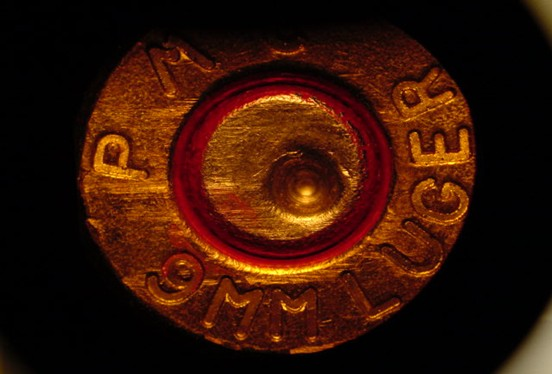
\includegraphics[width=.7\textwidth]{images/realCartridgeCaseImage} 

}

\caption{A fired 9mm Luger cartridge case with visible firing pin and breech face impressions.}\label{fig:realCartridgeCase}
\end{figure}

\hypertarget{an-overview-of-firearm-and-toolmark-examinations}{%
\subsubsection{An Overview of Firearm and Toolmark Examinations}\label{an-overview-of-firearm-and-toolmark-examinations}}

Trained firearm and toolmark examiners use a \emph{comparison microscope} like the one in Figure \ref{fig:comparisonMicroscope} to examine two pieces of evidence \citep{Zheng2014}.
A comparison microscope combines the view of two compound microscopes into a single view via an \emph{optical bridge}.
This allows an examiner to view two microscope stages simultaneously under the same eyepiece.
The right Figure \ref{fig:comparisonMicroscope} shows the view of two bullets under a comparison microscope.
The white dotted line represents the split in the two fields of view.
The goal of using a comparison microscope is to assess the ``agreement'' of the features on two pieces of evidence.

\begin{figure}[!htbp]

{\centering 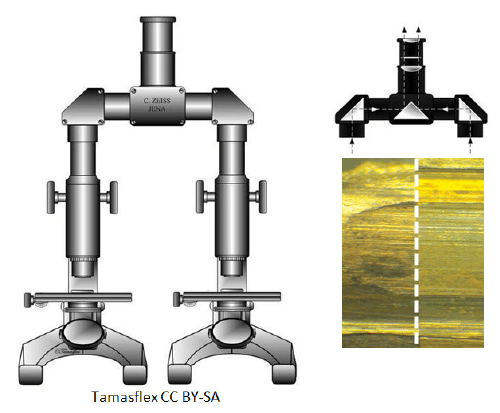
\includegraphics[width=.6\textwidth]{images/comparisonMicroscope} 

}

\caption{A comparison microscope consists of two stages upon which evidence is placed. These stages are placed under two compound microscopes that are joined together via an optical bridge and allow for viewing of both stages simultaneously under a single eyepiece. The image on the right shows an example of a bullet viewed under a comparison microscope.}\label{fig:comparisonMicroscope}
\end{figure}

Firearm examiners distinguish between three broad categories when characterizing the features of a fired bullet or cartridge case: class, subclass, and individual characteristics.
\emph{Class characteristics} are features associated with the manufacturing of the firearm such as the size of ammunition chambered by the firearm, the orientation of the extractor and ejector, or the width and twist direction of the barrel rifling.
An early step in a forensic examination is to determine the class characteristics of the firearm of origin as they can narrow the relevant population of potential firearm sources \citep{Thompson2017}.
For example, a 9mm cartridge case must have been fired by a firearm that can chamber 9mm ammunition.

If the discernible class characteristics match between two pieces of evidence, then the examiner uses a comparison microscope to compare the \emph{individual characteristics} of the evidence.
Individual characteristics are markings attributed to imperfections on the firearm surface due to the manufacturing process, use, and wear of the tool.
For example, markings on the breech face of a barrel often form after repeated fires of the firearm.
Individual characteristics are assumed to occur randomly across different firearms and therefore can be used to distinguish between two firearms.
The examiner independently rotates and translates the stages of a comparison microscope to find the position where the markings on the two pieces of evidence match \citep{Zheng2014}.
An examiner concludes that the evidence originated from the same firearm if the individual characteristics are in ``sufficient agreement'' \citep{AFTE1992}.

\emph{Subclass characteristics} exist between the macro-level class and micro-level individual characteristics.
These characteristics relate to markings reproduced across a subgroup of firearms.
For example, breech faces manufactured by the same milling machine may share similar markings \citep{firearmManufacturing}.
It can be difficult to distinguish between individual and subclass characteristics during an examination.
An examiner's decision process may be affected if the existence of subclass characteristics is suspected.

Many firearm and toolmark examiners in the United States adhere to the Association of Firearm and Toolmark Examiners (AFTE) Range of Conclusions when making their evidentiary conclusions \citep{AFTE1992}.
According to these guidelines, six possible conclusions can be made in a firearm and toolmark examination:

\begin{enumerate}
\def\labelenumi{\arabic{enumi}.}
\item
  \textbf{Identification}: Agreement of a combination of individual characteristics and all discernible class characteristics where the extent of agreement exceeds that which can occur in the comparison of toolmarks made by different tools and is consistent with the agreement demonstrated by toolmarks known to have been produced by the same tool.
\item
  \textbf{Inconclusive}: there are three possible inconclusive decisions
\end{enumerate}

\begin{quote}
2.1 Some agreement of individual characteristics and all discernible class characteristics, but insufficient for an identification.
\end{quote}

\begin{quote}
2.2 Agreement of all discernible class characteristics without agreement or disagreement of individual characteristics due to an absence, insufficiency, or lack of reproducibility.
\end{quote}

\begin{quote}
2.3 Agreement of all discernible class characteristics and disagreement of individual characteristics, but insufficient for an elimination.
\end{quote}

\begin{enumerate}
\def\labelenumi{\arabic{enumi}.}
\setcounter{enumi}{2}
\item
  \textbf{Elimination}: Significant disagreement of discernible class characteristics and/or individual characteristics.
\item
  \textbf{Unsuitable}: Unsuitable for examination.
\end{enumerate}

Forensic examinations first involve an examination of a ``questioned'' bullet or cartridge case for identifiable toolmarks \citep{Thompson2017}.
The examiner classifies markings by their class, individual, and subclass characteristics.
The examiner compares these characteristics to ``known source'' fires obtained from a suspect's firearm if one is available.
Otherwise, class characteristics from the questioned bullet can be used to narrow the relevant population and provide potential leads.
An examiner's decision may be used as part of an ongoing investigation or presented at trial as expert testimony.

Standard operating procedures for assessing and comparing evidence differ between forensic laboratories.
For example, some labs collapse the three possible inconclusive decisions into a single decision \citep{Neuman2022} or prohibit examiners from making an elimination based on differences in individual characteristics \citep{Duez2017}.

\hypertarget{why-should-firearm-and-toolmark-identification-change}{%
\subsection{Why Should Firearm and Toolmark Identification Change?}\label{why-should-firearm-and-toolmark-identification-change}}

In 2009, the National Research Council released a report assessing a number of forensic disciplines including Firearm and Toolmark analysis.
The report pointed out that firearm and toolmark analysis lacked a precisely defined process and that little research had been done to determine the reliability or repeatability of the methods.
\emph{Reliability} refers to the ability to correctly classify evidence as originating from the same source or not.
\emph{Repeatability} refers to the consistency of conclusions; for example, whether an examiner makes the same conclusion if presented with the same evidence on different occasions.
Two of the recommendations from this study were to establish rigorously-validated laboratory procedures and ``develop automated techniques capable of enhancing forensic technologies \citep{council_strengthening_2009}.''

A number of studies assess the reliability and repeatability of a firearm and toolmark examination (non-exhaustively: \citet{DeFrance2003,Hamby2009,fadulempirical2011,Stroman2014,Baldwin2014,Smith2016,MATTIJSSEN2020}).
These studies indicate that examiners have a low error rate when comparing evidence obtained under controlled conditions (i.e., for which ground-truth is known).
However, as pointed out in a 2016 report from the President's Council of Advisors on Science and Technology, many of these studies, save \citet{Baldwin2014}, were not ``appropriately designed to test the foundational validity and estimate reliability \citep{pcast2016}.''
The report called for more properly-designed studies to establish the scientific validity of the discipline.

Due to the opacity in the decision-making process, examiners are referred to as ``black boxes'' in a similar sense to black-box algorithms \citep{HumanFactorsCommittee2020}.
Their evidentiary conclusions are fundamentally subjective and empirical evidence suggests that conclusions may differ if examiners are presented with the same evidence on different occasions \citep{Ulery2011,Ulery2012}.
Examiners rarely need to provide quantitative justification for their conclusion.
Even for qualitative justifications, it can be difficult to determine what the examiner is actually ``looking at'' to arrive at their conclusion \citep{Ulery2014}.
This suggests the need to supplement these black box decisions with transparent, objective techniques that quantitatively measure the similarity between pieces of evidence.
As stated in \citet{pcast2016}, efforts should be made to ``convert firearms analysis from a subjective method to an objective method'' including ``developing and testing image-analysis algorithms for comparing the similarity of tool marks.''
This work focuses on the development of an algorithm for comparing breech face impressions on cartridge cases.

\hypertarget{forensic-comparison-pipelines}{%
\section{Forensic Comparison Pipelines}\label{forensic-comparison-pipelines}}

Recent work in many forensic disciplines has focused on the development of algorithms to measure the similarity between pieces of evidence including glass \citep{Curran2000-hp,Park2019,openForSciR}, handwriting \citep{crawford_handwriting_2020}, shoe prints \citep{park_algorithm_2020}, ballistics \citep{hare_automatic_2016,tai_fully_2018}, and toolmarks \citep{Hadler2017,Krishnan2018}.
These algorithms often result in a numerical score for two pieces of evidence.
A numerical score can add more nuance to an evidentiary conclusion beyond simply stating whether the evidence originated from the same source as would be the case in binary classification.
For example, a larger similarity scores implies the evidence is more similar.
However, an examiner must ultimately reach one of two conclusions (or three, if admitting inconclusives).
Whether a conclusion should be based solely on an algorithm's similarity score or if an examiner should incorporate the similarity score into their own decision-making process is still up for debate \citep{Swofford2021}.
In this work we view forensic comparison algorithms as a supplement to, rather than a replacement of, the traditional forensic examination.

We treat forensic comparison algorithms as evidence-to-classification ``pipelines.''
Broadly, the steps of the pipeline include \citet{Rice2020}:

\begin{enumerate}
\def\labelenumi{\arabic{enumi}.}
\item
  capturing a digital representation of the evidence,
\item
  pre-processing this representation to isolate or emphasize a region of interest of the evidence,
\item
  comparing regions of interest from two different pieces of evidence to obtain a (perhaps high-dimensional) set of similarity features,
\item
  combining these features into a low-dimensional set of similarity scores, and
\item
  defining a classification rule based on these similarity features.
\end{enumerate}

We add to this structure the emphasis that each step of the pipeline can be further broken-down into modularized pieces.
For example, the pre-processing step may include multiple sub-procedures to isolate a region of interest of the evidence.
Figure \ref{fig:pipelineDiagram} shows two possible variations of the cartridge case comparison pipeline as well as the parameters requiring manual specification and alternative modules.
The benefits of this modularization include easing the process of experimenting with different parameters/sub-procedures and improving the comprehensibility of the pipeline.

\begin{figure}[!htbp]

{\centering 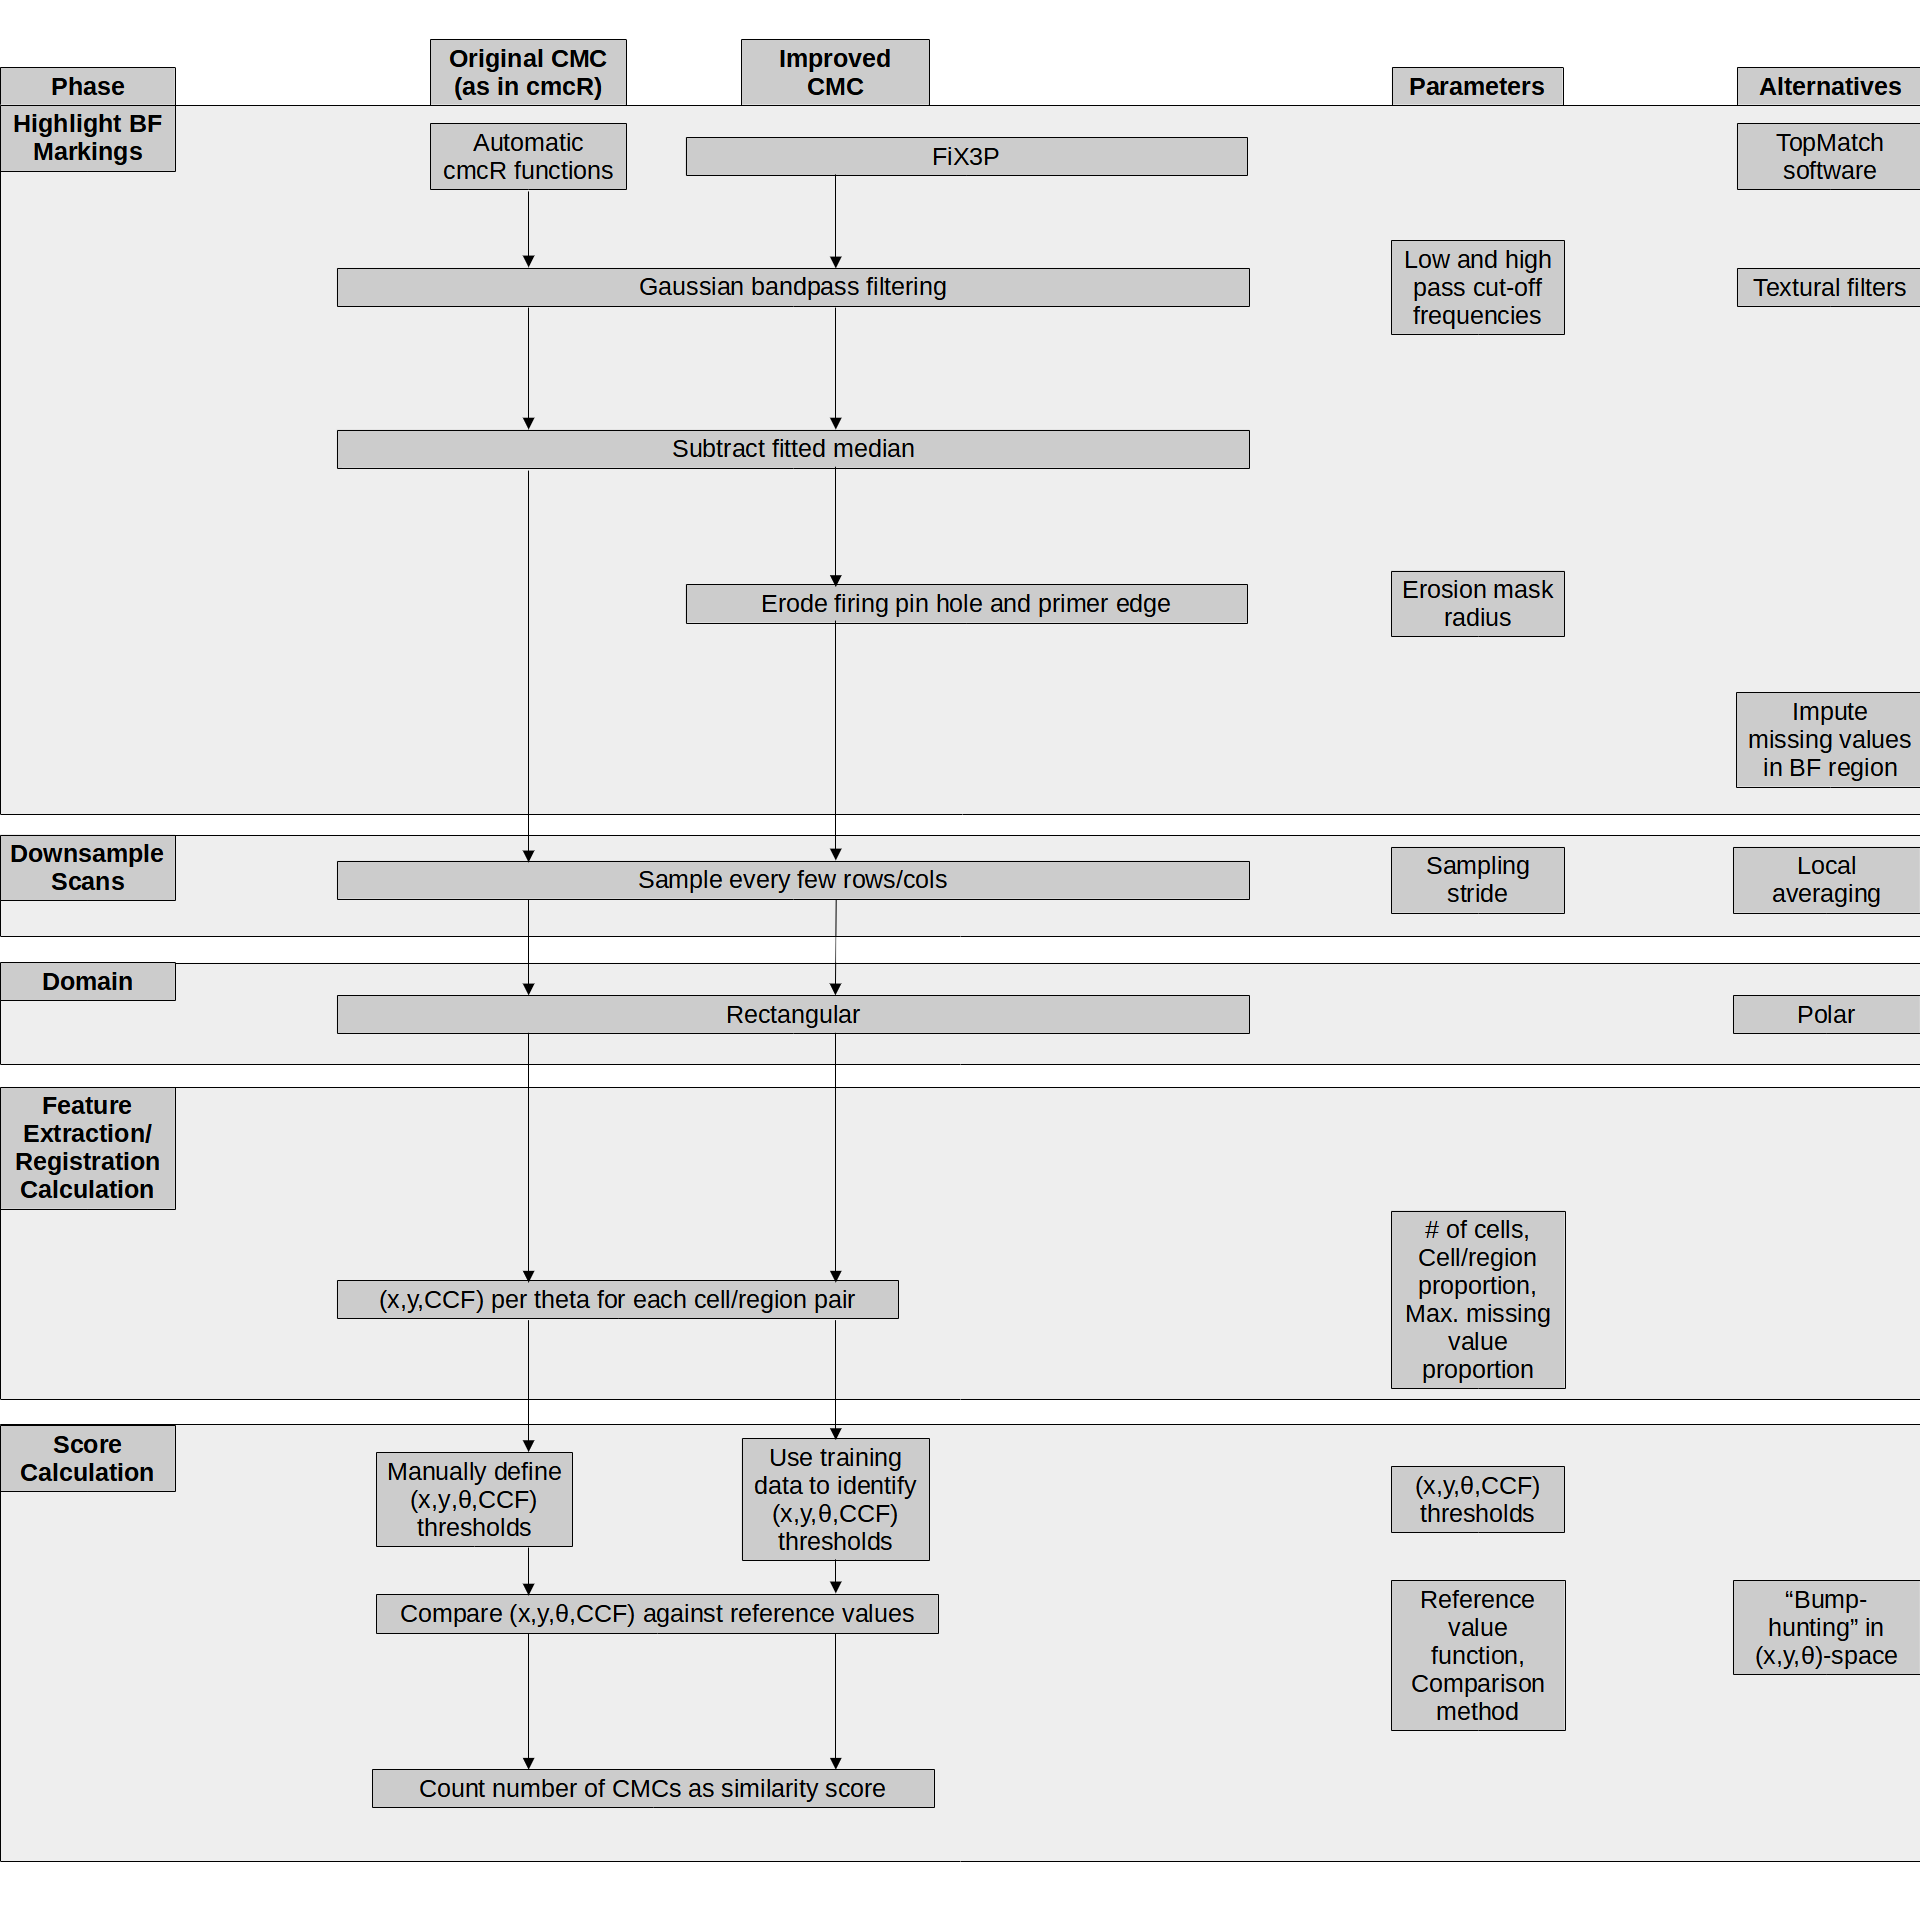
\includegraphics[width=\textwidth]{images/pipelineDiagram_6-8-22} 

}

\caption{Variations upon the cartridge case comparison pipeline. The first two columns detail the pipeline with different sub-procedures. The third columns shows the parameters that require manual specification at each step. The fourth column shows  alternative processing steps that could replace steps in the existing pipeline.}\label{fig:pipelineDiagram}
\end{figure}

In the following sections, we detail recent advances to each of the five steps in the pipeline outlined above.
We narrow our focus to advances made in comparing firearms evidence.

\hypertarget{digital-representations-of-evidence}{%
\subsection{Digital Representations of Evidence}\label{digital-representations-of-evidence}}

Digital representations of cartridge case evidence commonly come in two forms: 2D optical images or 3D topographic scans.
A common way to take 2D optical images is to take a picture of the cartridge case surface lit up under a microscope, implying a dependence on the lighting conditions under which the picture was taken.
Some recent work has focused on comparing 2D optical images \citep{tai_fully_2018,tong_fired_2014}, although the use of 3D microscopes has recently become more prevalent to capture the surface of ballistics evidence.

Using a 3D microscope allows for the scanning of surfaces at the micron (or micrometer) level under light-agnostic conditions \citep{weller_2012}.
Figure \ref{fig:cartridgeCaseImages} shows a 2D image and 3D topography of the same cartridge case primer from \citet{fadulempirical2011}.

\begin{figure}[!htbp]

{\centering 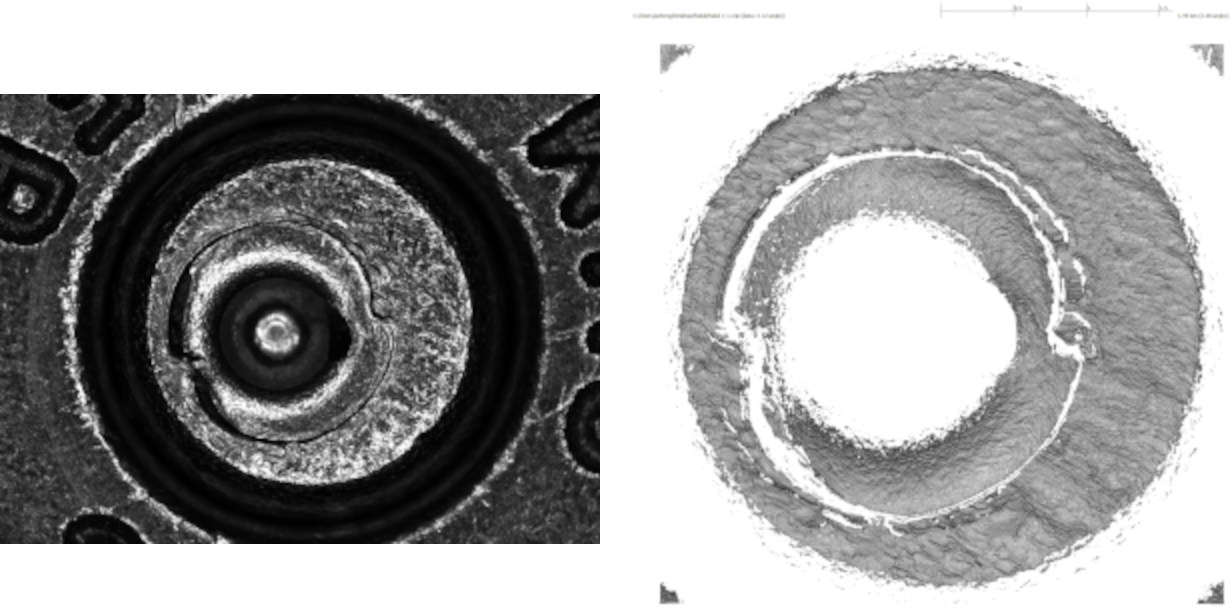
\includegraphics[width=\textwidth]{images/fadul1-1_sidebyside} 

}

\caption{A cartridge case captured using 2D confocal reflectance microscopy (left) and 3D disc scanning confocal microscopy (right).}\label{fig:cartridgeCaseImages}
\end{figure}

Recently, Cadre Forensics\texttrademark introduced the TopMatch-3D High-Capacity Scanner \citep{topmatch}.
Figure \ref{fig:topMatchScanner} shows a TopMatch scanner with a tray of 15 fired cartridge cases \citep{topmatchFlyer}.
This scanner collects images of a gel pad under various lighting conditions into which the cartridge case surface is impressed. Proprietary algorithms combine these images into a regular 2D array called a \emph{surface matrix}.
Elements of the surface matrix represent the relative height value of the associated surface.\\
The physical dimensions of these scans are about 5.5 \(mm^2\) captured at a resolution of 1.84 microns per pixel (1000 microns equals 1 mm).

\begin{figure}[!htbp]

{\centering 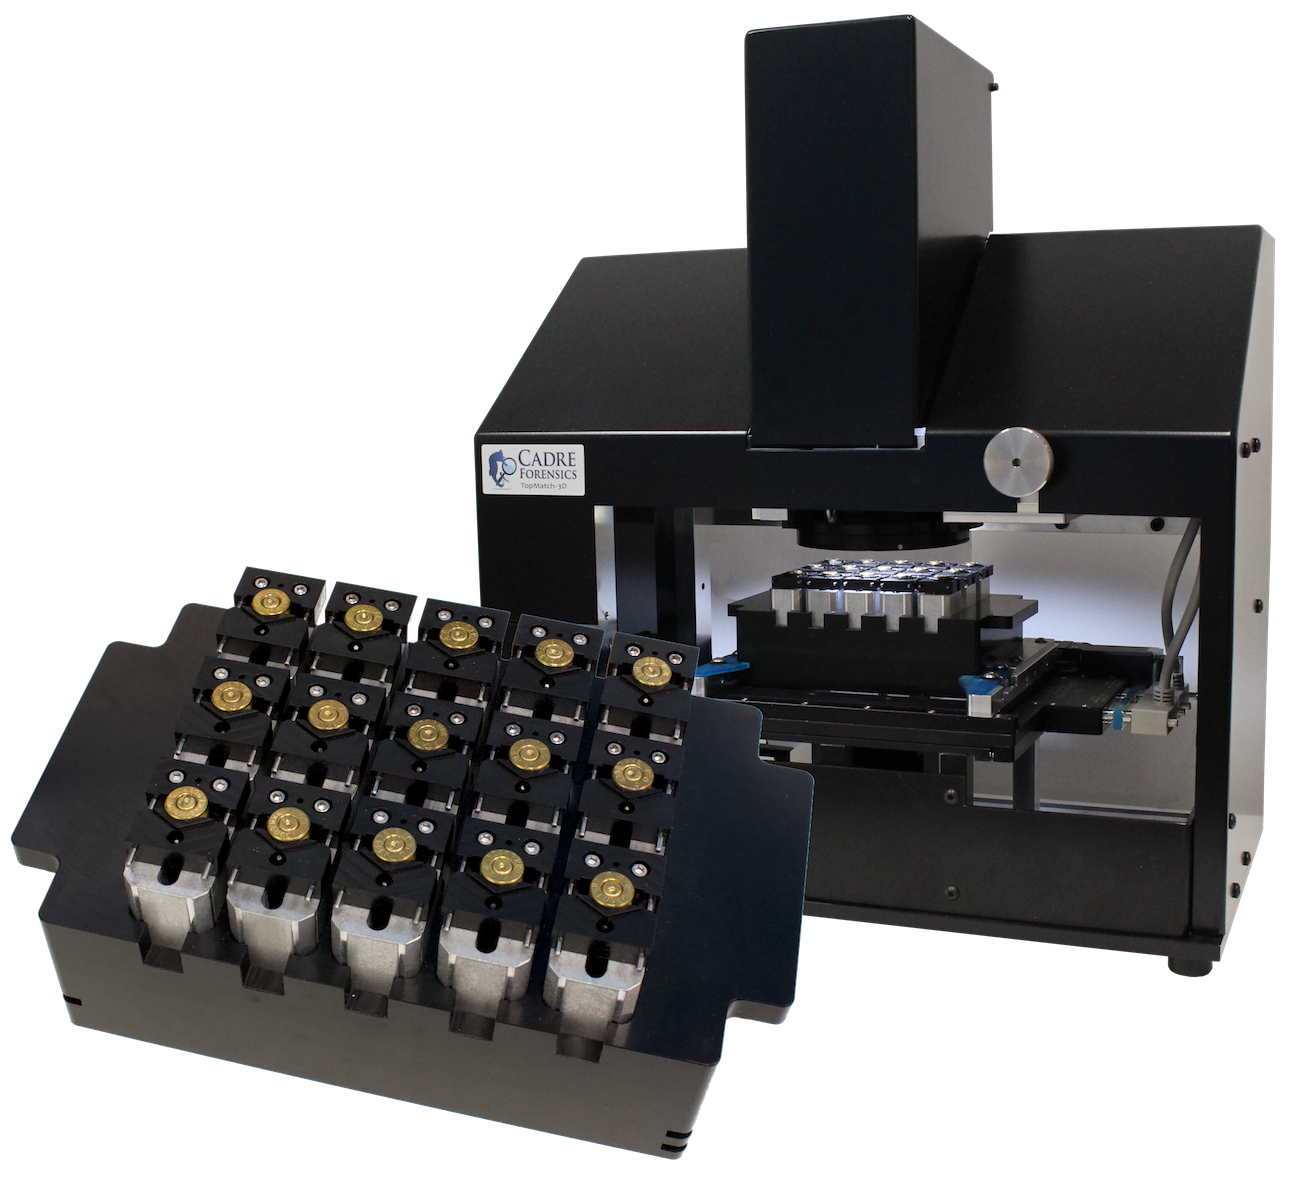
\includegraphics[width=.7\textwidth]{images/TopMatchSystem7} 

}

\caption{The TopMatch-3D High-Capacity Scanner from Cadre Forensics\texttrademark\ . The scanner captures topographic scans of a gel pad into which a cartridge case surface is impressed.}\label{fig:topMatchScanner}
\end{figure}

The ISO standard x3p file format is commonly used to save 3D scans \citep{ISO25178-72}.
An x3p is a container consisting of a single surface matrix representing the height values of the surface and metadata concerning the parameters under which the scan was taken as shown in Figure \ref{fig:x3pFlowchart} \citep{Zheng2020}.
A number of studies suggest that 3D topographic scans of cartridge case surfaces lead to more accurate classifications than 2D optical images of the same evidence \citep{Tai2019,tong_fired_2014,song_3d_2014}.

\begin{figure}[!htbp]

{\centering 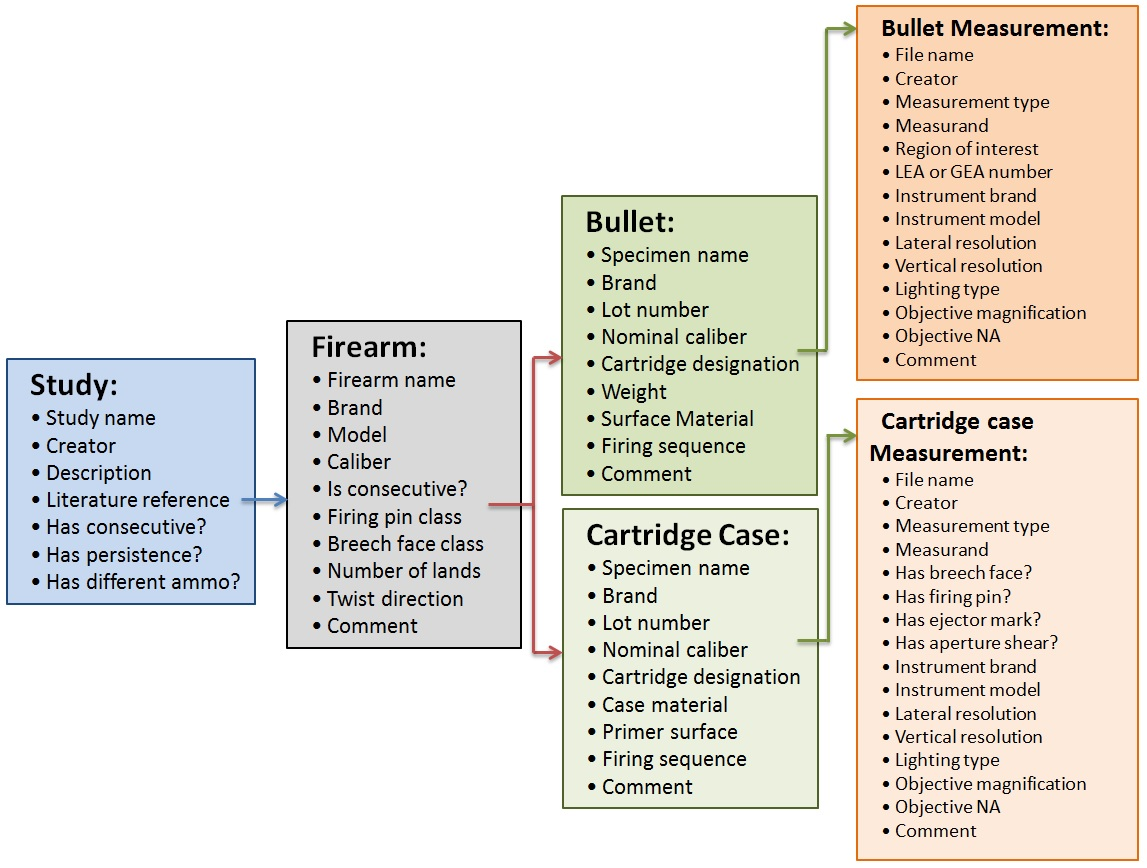
\includegraphics[width=.7\textwidth]{images/x3pFlowchart} 

}

\caption{The hierarchy of information stored in the x3p file format for both bullet and cartridge case evidence.}\label{fig:x3pFlowchart}
\end{figure}

\hypertarget{pre-processing-procedures-for-forensic-data}{%
\subsection{Pre-processing Procedures for Forensic Data}\label{pre-processing-procedures-for-forensic-data}}

After obtaining a surface's digital representation, we next want to isolate regions of the surface containing distinguishable markings.
Figure \ref{fig:cartridgeCaseImages} shows an example of a 2D image and 3D scan of the same cartridge case.
In both representations, the corners of these arrays include regions of the cartridge case surface outside of the primer.
The center of the cartridge case primer contains an impression left by the firing pin during the firing process.
We wish to isolate the annular breech face region around the firing pin impression from the rest of the captured surface.

Both the 2D optical and 3D topographic representations of cartridge case surfaces are fundamentally pictorial in nature.
As such, breech face impression isolation commonly relies on image processing and computer vision techniques.
\citet{tai_fully_2018} uses a combination of histogram equalization, Canny edge detection, and morphological operations to isolate breech face impressions in 2D images.
A Gaussian filter is another common tool to emphasize breech face impressions.
\citet{tong_fired_2014} apply a low-pass Gaussian filter to remove noise via a Gaussian-weighted moving average operation.
\citet{chu_validation_2013} and \citet{song_estimating_2018} use a bandpass Gaussian filter to simultaneously remove noise and unwanted global structure from the scan.
\citet{song_3d_2014} and \citet{chen_convergence_2017} use a ``robust'' variant of the Gaussian filter to omit outliers from the scan \citep{ISO16610-71}.

Instead of automatic procedures, others have used subjective human intervention to isolate the breech face impressions.
For example, \citet{song_estimating_2018} performed ``manually trimming to extract the breech face impression of interest'' on a set of cartridge case scans.
In \citet{Roth2015}, examiners manually identify the borders of the breech face impression region by placing points around an image of the cartridge case primer.

\hypertarget{forensic-data-feature-extraction}{%
\subsection{Forensic Data Feature Extraction}\label{forensic-data-feature-extraction}}

After isolating the breech face impressions, we compare two pre-processed cartridge case scans and compute a set of similarity features.
Because the cartridge cases at this point are represented as high-dimensional matrices, this process can be thought of as a dimensionality reduction of the high-dimensional surface arrays to a set of similarity statistics.

A variety of features have been proposed to quantify the similarity between two cartridge case surface arrays.
\citet{tai_fully_2018} propose calculating the cross-correlation function (CCF) value between two cartridge cases across a grid of rotations.
The cross-correlation function measures the similarity between two matrices for every translation of one matrix against the other.
For two matching cartridge cases, we assume that the CCF will be largest after aligning the cartridge cases surfaces by their shared breech face impressions.
Conversely, we expect the CCF to be relatively small for two non-matching cartridge cases no matter the alignment.
\citet{Riva2014} propose combining the CCF between two aligned scans with the element-wise median Euclidean distance and median difference between the normal vectors at each point of the surface.
\citet{Riva2016} and \citet{Riva2020} applied Principal Component Analysis to reduce these three features down to two principal components for the sake of fitting a 2D kernel density estimator.

Pertinent to this work is the cell-based comparison procedure originally outlined in \citet{song_proposed_2013}.
The underlying assumption of \citet{song_proposed_2013} is similar to that of \citet{tai_fully_2018}: that two matching cartridge cases will exhibit higher similarity when they are close to being correctly aligned.
While \citet{tai_fully_2018} measured similarity using the CCF between the two full scans, \citet{song_proposed_2013} proposes partitioning the scans into a grid of ``correlation cells'' and counting the number of similar cells between the two scans.
The rationale behind this procedure is that many cartridge case scans have only a few regions with discriminatory markings.
As such, comparing full scans may result in a lower correlation than if one were to focus on the highly-discriminatory regions.
In theory, dividing the scans into cells allows for the identification of these regions.
After breaking a scan into a grid of cells, each cell is compared to the other scan to identify the rotation and translation, known together as the \emph{registration}, at which the cross-correlation is maximized.
\citet{song_proposed_2013} assumes that the cells from a truly matching pair of cartridge cases will ``agree'' on their registration in the other scan.
\citet{song_proposed_2013} referred to the procedure of counting the number of similar cells the ``Congruent Matching Cells'' method.
Chapter 2 contains more details of this procedure.

\hypertarget{similarity-scores-classification-rules-for-forensic-data}{%
\subsection{Similarity Scores \& Classification Rules for Forensic Data}\label{similarity-scores-classification-rules-for-forensic-data}}

Following feature extraction, the dimensionality of these features is further reduced to a low-dimensional, usually univariate, similarity score.
We can define a decision boundary based on the value of the similarity score to classify cartridge case pairs as matching or non-matching.

After calculating the CCF across various possible registrations, \citet{tai_fully_2018} propose using the maximum observed CCF value as the univariate similarity score.
They perform binary classifications by setting a CCF threshold above which pairs are classified as ``matches'' and below which as ``non-matches.''
\citet{Tai2019} proposes setting a CCF cut-off that maximizes the precision and recall in a training set of pairwise comparisons.

\citet{Riva2016,Riva2020} use a training set to fit two 2D kernel density estimates to a set of features from matching and non-matching comparisons.
Using these estimates, they compute a score-based likelihood ratio (SLR), which can be interpreted as a similarity score \citep{Garton2021}.

For the Congruent Matching cells method, \citet{song_proposed_2013} proposes using the number of cells that agree on a registration, the ``congruent matching'' cells, as a similarity score.
The criteria used to define ``congruent matching'' cells has changed across papers \citep{song_3d_2014,tong_fired_2014,tong_improved_2015,chen_convergence_2017} and will be discussed in greater detail in Chapter 2.
The authors of these papers have consistently used six congruent matching cells as a decision boundary to distinguish matching and non-matching cartridge case pairs.

\citet{Zhang2020} applies the Density-Based Spatial Clustering of Applications with Noise (DBSCAN) algorithm \citep{Ester1996} to the features from the cell-based comparison procedure to determine if any clusters form amongst the per-cell estimated registration values.
This is based on the assumption that any cells that come to a consensus on their registration should form a cluster in translation \((x,y)\) and rotation \(\theta\) space.
\citet{Zhang2020} proposes a binary classifier based on whether any clusters are identified by the DBSCAN algorithm \citep{Ester1996}.
If a cluster is found for a particular pairwise comparison, then that pair is classified as a ``match'' and otherwise as a ``non-match.''

Apart from the algorithms described in \citet{tai_fully_2018} and \citet{Tai2019}, the authors of these comparison algorithms have not provided publicly available code or data.
As such, although the results reported in associated papers are promising, it is difficult or impossible for other researchers to verify or reproduce the findings.
Results must be reproducible to be accepted by others in any scientific domain.
In the next section, we discuss recent challenges and opportunities in computationally reproducible research.

\hypertarget{reproducibility-of-comparison-pipelines}{%
\subsection{Reproducibility of Comparison Pipelines}\label{reproducibility-of-comparison-pipelines}}

\citet{nasem_2019} defines \emph{reproducibility} as ``obtaining consistent computational results using the same input data, computational steps, methods, code, and conditions of analysis.''
While not exact in their definition of ``consistent,'' the authors assert that, barring a few exceptions, it is reasonable to expect that the results obtained by a second researcher, after applying the exact same processing steps to the exact same data, be the exact same as the original results.
In either case, they assert that ``a study's data and code have to be available in order for others to reproduce and confirm results.''
Given data and code, researchers are able to verify the results, incorporate the materials into their own research, and improve or accelerate discovery \citep{Stodden2018b}.

A number of studies indicate that computationally reproducible research is sparse across various disciplines.
\citet{Stodden2018b} and \citet{Stodden2018a} studied the reproducibility of articles sampled from the \emph{Journal of Computational Physics} and the journal \emph{Science}, respectively.
In the former, \citet{Stodden2018b} found that zero of 306 randomly selected articles from the \emph{Journal of Computaional Physics} were ``straightforward to reproduce with minimal effort'' and, at best, that five articles were ``reproducible after some tweaking.''
In the latter, \citet{Stodden2018a} found that only 3 of 204 randomly selected articles from \emph{Science} were ``straightforward to reproduce with minimal effort;'' despite a journal policy requiring that all code and data used in the paper be made available to any reader.
Similar findings were found in \citet{CChang2022} (29 of 59 economic papers reproducible), \citet{Iqbal2016} (zero of 268 biomedical papers provided raw data and 1 in 268 linked to a full study protocol), \citet{Duvendack2015} (50\% or more published articles include data or code in only 27 of 333 economics journals), and \citet{Gundersen2018} (24 of 400 AI conference papers included code).
A common recommendation amongst these authors is to establish of rigorous tools and standards to promote reproducibility.
This includes making code and data used in a paper easily-accessible to readers.

Infrastructure already exists to ease the process of developing, maintaining, and sharing open-source code and data.
Data repositories such as the NIST Ballistics Toolmark Research Database \citep{Zheng2020} provide open access to raw data.
\citet{Grning2018} discuss the use of package managers such as Conda (\url{https://anaconda.org/anaconda/conda}), container software such as Docker (\url{https://www.docker.com/}), and virtual machine software to preserve the entire data analysis environment in-perpetuity.
For situations in which VMs or containers aren't available, software such as the \texttt{manager} R package allows users to ``compare package inventories across machines, users, and time to identify changes in functions and objects \citep{Rice2020}.''
\citet{Piccolo2016} reference repositories like Bioconductor \citep{Huber2015} that make it easy to document and distribute code.
Further, software such as the \texttt{knitr} R package \citep{Xie2014} enable ``literate programming'' in which prose and executed code can be interwoven to make it easier to understand the code's function.
These tools make data, code, and derivative research findings more accessible, in terms of both acquisition and comprehensibility, to consumers and fellow researchers.

\hypertarget{diagnostic-tools}{%
\section{Diagnostic Tools}\label{diagnostic-tools}}

Forensic examiners often provide expert testimony in court cases.
As part of this testimony, an examiner is allowed to provide facts about the outcome of a forensic examination and their opinion about what the results mean.
A party to a court may challenge the examiner on the validity of the underlying scientific method or whether they interpreted the results correctly \citep{aafsArticle}.
In these situations, examiners need to explain the process by which they reached an evidentiary conclusion to the fact finders of the case; namely, the judge or jury.
As algorithms are more often used in forensic examinations, the technical knowledge required to understand and explain an algorithm to lay-people has increased.
Indeed, even the most effective algorithms may be moot if an examiner can't explain the algorithm in their testimony.
While in some cases the authors of the algorithm have been willing to provide testimony to establish the validity of the algorithm \citep{trueAlleleTestimony}, this will become less viable as algorithms become more prevalent.

The resources required to educate examiners on the theory and implementation of highly technical algorithms makes additional training seem currently implausible.
An alternative is to develop algorithms from the ground-up to be intuitive for examiners to understand and explain to others.
\emph{Explainability} refers to the ability to identify the factors that contributed to the results of an algorithm \citep{Belle2021PrinciplesAP}.
For example, understanding why a classifier predicted one class over another.
\emph{Diagnostics} are tools to explain or justify the behavior of a model or algorithm in specific instances.
Myriad diagnostic tools exist to explain the results of an algorithm.
These range from identifying instances of the training set that illuminate how the model operates \citep{Deng2018} to fitting more transparent models that accurately approximate the complex model \citep{Puiutta2020} to explaining the behavior of the algorithm in a small region of interest of the prediction space \citep{LIME,Goode2021}.
Many of these methods require additional technical knowledge to interpret these explanations.

\hypertarget{visual-diagnostics}{%
\subsection{Visual Diagnostics}\label{visual-diagnostics}}

A less technical approach is to use visualizations that facilitate understanding of model behavior.
Properly constructed visuals enable both exploratory data analysis and diagnostics \citep{Buja2009}, which are critical steps in the data analysis process for anticipating and assessing model fit.
Given that many of the procedures by which cartridge case evidence is captured, processed, and compared are based on image processing techniques, a visual diagnostic is an intuitive mode of explanation for researchers and lay-people alike.
As stated in \citet{cleveland1994elements}, ``graphical methods tend to show data sets as a whole, allowing us to summarize the behavior and to study detail. This leads to much more thorough data analyses.''

Numerical statistics summarize the behavior of data, but miss the detail referenced in Cleveland's quote \citep{telea2014data}.
To illustrate this, consider the famous data sets from \citep{Anscombe1973} known as Anscombe's quartet.
The two variables in each data set are plotted against one another in Figure \ref{fig:anscombeQuartet}.
There are clear differences in the relationship between \texttt{x} and \texttt{y} across these four data sets.

\begin{figure}[!htbp]

{\centering 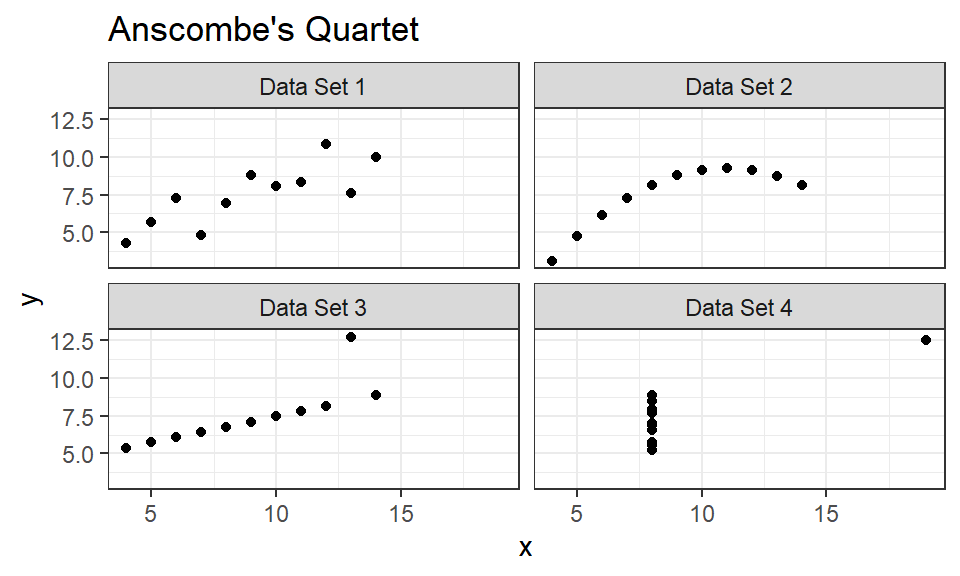
\includegraphics{thesis_files/figure-latex/anscombeQuartet-1} 

}

\caption{A visualization of Anscombe's quartet. Despite there being obvious differences between these four data sets, their summary statistics are nearly identical}\label{fig:anscombeQuartet}
\end{figure}

Despite these differences, Table \ref{tab:anscombeStats} shows that summary statistics, namely the first two moments, are identical.
This demonstrates that visual diagnostics can be more effective at uncovering data behavior than summary statistics (at least low-order moments).

\begin{table}[!htbp]
\centering
\begin{tabular}{| r | r | r | r | r |}
\hline
Data Set & $\bar{x}$ & S.D. $x$ & $\bar{y}$ & S.D. $y$ \\
\hline
1 & 9 & 3.32 & 7.5 & 2.03 \\
\hline
3 & 9 & 3.32 & 7.5 & 2.03 \\
\hline
3 & 9 & 3.32 & 7.5 & 2.03 \\
\hline
4 & 9 & 3.32 & 7.5 & 2.03 \\
\hline
\end{tabular}
\caption{Moments of the two variables in Anscombe's quartet.}
\label{tab:anscombeStats}
\end{table}

Given the pivotal role that visual diagnostics play in the data analysis pipeline, we now consider best practices in creating data visualizations.
Human brains are wired for seeing patterns and differences, and for understanding spatial relationships from this \citep{telea2014data}.
As such, an effective visual diagnostic or data visualization is one that conveys patterns quickly and easily, and with minimal scope for understanding.
Arising originally from a psychological theory of perception, the Gestalt Laws of Perceptual Organization \citep{Goldstein2016-un} summarize important considerations when constructing statistical graphics.
The Gestalt laws are as follows:

\begin{itemize}
\item
  \textbf{Pragnanz - the law of simplicity:} Every stimulus pattern is seen in such a away that the resulting structure is as simple as possible.
\item
  \textbf{Proximity:} Things that are near each other appear to be grouped together.
\item
  \textbf{Good Continuation:} Points that, when connected, result in straight or smoothly curving lines are seen as belonging together, and the lines tend to be seen in such a way as to follow the smoothest path.
\item
  \textbf{Similarity:} Similar things appear to be grouped together.
\item
  \textbf{Common Region:} Elements that are within the same region of space appear to be grouped together.
\item
  \textbf{Uniform Connectedness:} A connected region of visual properties, such as the lightness, color, texture, or motion, is perceived as a single unit.
\item
  \textbf{Synchrony:} Visual events that occur at the same time are perceived as belonging together.
\item
  \textbf{Common Fate:} Things that are moving in the same direction appear to be grouped together.
\item
  \textbf{Familiarity:} Things that form patterns that are familiar or meaningful are likely to become grouped together.
\end{itemize}

These laws provide guidance on how to construct a visual that concisely conveys a pattern or difference in data.
For data visualization, additional laws include \citep{Midway2020}:

\begin{itemize}
\item
  \textbf{Use and Effective Geometry:} Choose a geometry (shape and features of a statistical graphic) that is appropriate to the data.
\item
  \textbf{Colors Always Mean Something:} Colors in visuals can convey groupings or a range of values.
\end{itemize}

Figure \ref{fig:chickweightExample} depicts a case study of the Gestalt principles in practice.
The plot shows the weight over time of chicks fed one of two experimental diets \citep{crowder1990analysis}.
Individual points represent the weight of a single chick on a particular day.
Connected points represent the weight for a single chick over time.
This is an example of using an effective geometry (point \& line graph to represent time series) along with the Gestalt law of Good Continuation.
We further apply the Gestalt law of Common Region to facet the data set into plots based on diet.
This implicitly communicates to the audience that the weights of two diet groups of chicks is expected to differ.
Indeed, appealing to the Gestalt law of Uniform Connectedness, the ``motion'' of the grouped time series suggests that chicks given Diet 2 tend to gain weight more rapidly than those given Diet 1.
This may suggest a particular modeling structure for these time series (e.g., diet fixed effect) or the need to assess the experimental design to ensure that the assumption that the chicks were randomly sampled from the same population is appropriate.
We see how such a plot can be used for both exploratory data analysis or as a post-hoc diagnostic tool.
Alternative to faceting, the time series from these two diet groups could be combined into a single plot and distinguished by color.

\begin{figure}[!htbp]

{\centering 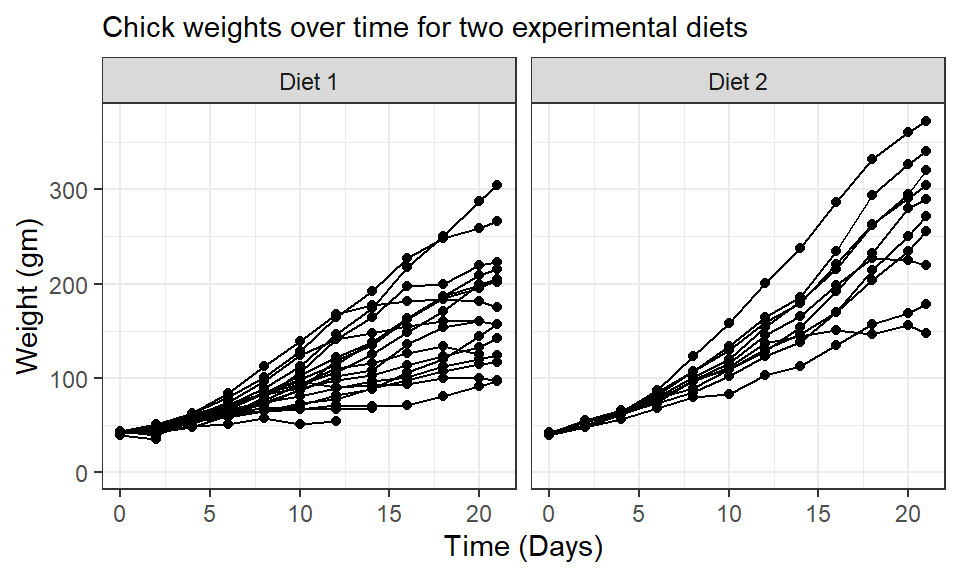
\includegraphics{thesis_files/figure-latex/chickweightExample-1} 

}

\caption{An example of a statistical graphic that uses the Gestalt Laws of Perceptual Organization to communicate data findings.}\label{fig:chickweightExample}
\end{figure}

The R programming language \citep{r} provides a variety of tools to create visual diagnostics.
Among the most robust of these tools is the ggplot2 package \citep{ggplot2}.
This package extends the ``Grammar of Graphics'' introduced in \citet{Wilkinson2005} to provide a user-friendly structure to create statistical graphics.
We use the \texttt{+} operator to ``layer'' features of a statistical graphic (e.g., elements, transformations, guides, labels) on a blank canvas.
\ref{fig:ggplot2Example} along with the accompanying code chunk demonstrates how to create a residual plot from a simple linear regression using the ggplot2 package.
This visual diagnostic allows the analyst or audience to determine whether the homoscedasticity or linear form assumptions underlying simple linear regression are met.
For those willing to learn the ``grammar,'' the code used to create these statistical graphics can easily be re-used and tweaked to fit a specific application.
1

\begin{Shaded}
\begin{Highlighting}[]
\NormalTok{lmFit }\OtherTok{\textless{}{-}} \FunctionTok{lm}\NormalTok{(}\AttributeTok{formula =}\NormalTok{ rating }\SpecialCharTok{\textasciitilde{}}\NormalTok{ complaints,}\AttributeTok{data =}\NormalTok{ datasets}\SpecialCharTok{::}\NormalTok{attitude)}

\FunctionTok{library}\NormalTok{(ggplot2)}

\FunctionTok{ggplot}\NormalTok{(}\AttributeTok{data =} \FunctionTok{data.frame}\NormalTok{(}\AttributeTok{Complaints =}\NormalTok{ datasets}\SpecialCharTok{::}\NormalTok{attitude}\SpecialCharTok{$}\NormalTok{complaints,}
                         \AttributeTok{Residuals =}\NormalTok{ lmFit}\SpecialCharTok{$}\NormalTok{residuals)) }\SpecialCharTok{+}
  \FunctionTok{geom\_point}\NormalTok{(}\FunctionTok{aes}\NormalTok{(}\AttributeTok{x =}\NormalTok{ Complaints,}\AttributeTok{y =}\NormalTok{ Residuals)) }\SpecialCharTok{+}
  \FunctionTok{geom\_hline}\NormalTok{(}\AttributeTok{yintercept =} \DecValTok{0}\NormalTok{,}\AttributeTok{linetype =} \StringTok{"dashed"}\NormalTok{) }\SpecialCharTok{+}
  \FunctionTok{labs}\NormalTok{(}\AttributeTok{x =} \StringTok{"\% in{-}favor of handling of employee complaints"}\NormalTok{)}
\end{Highlighting}
\end{Shaded}

\begin{figure}[!htbp]

{\centering 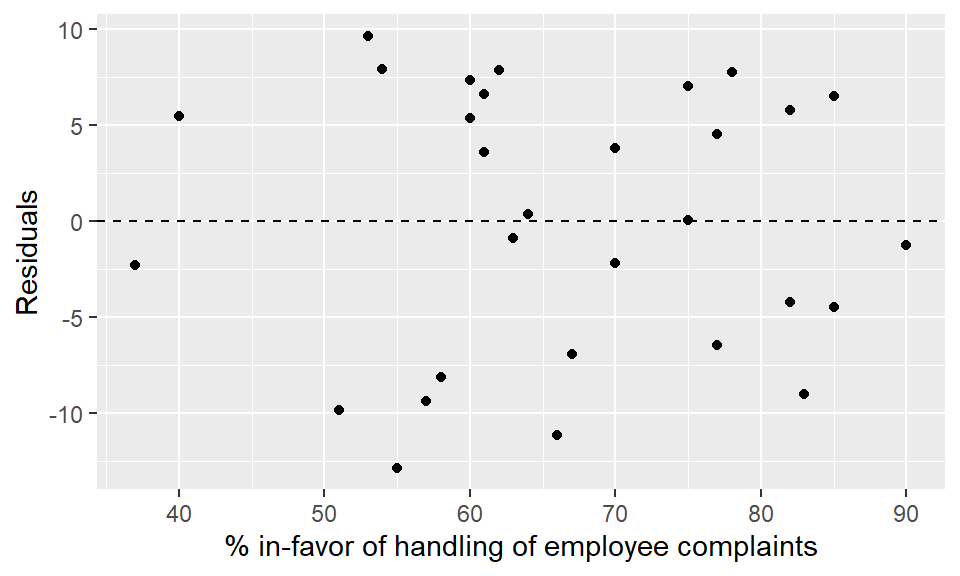
\includegraphics{thesis_files/figure-latex/ggplot2Example-1} 

}

\caption{An example of using the ggplot2 package to construct a residual plot from a simple linear regression. The features of the statistical graphic are combined layer-by-layer using the + operator as we see in the accompanying code chunk.}\label{fig:ggplot2Example}
\end{figure}

Properly constructed visual diagnostics provide the audience with a nuanced yet intuitive explanation of the behavior of a model or algorithm that summary diagnostic statistics may not convey.
Tools like the ggplot2 package provide a coherent, thorough infrastructure for creating such visual diagnostics.
However, the tools discussed thus far are useful for creating \emph{static} visualizations.
In the next section, we discuss the benefits of making a visual diagnostic interactive to user input.

\hypertarget{interactive-diagnostics}{%
\subsection{Interactive Diagnostics}\label{interactive-diagnostics}}

Interactive diagnostic tools encourage both expert and lay users to engage with an analysis pipeline that otherwise may be technically or conceptually inaccessible.
Rather than answering a question posed by the author of a plot as a static plot does, such interactive diagnostic tools enable the audience to formulate and answer their own questions.
This leads to deeper engagement with the data \citep{telea2014data}.
While the ggplot2 package eases the process of constructing visual diagnostics, software such as the shiny R package \citep{shiny} enables the consumer of the diagnostic to interact with the visualizations and underlying data.
The shiny package provides tools for using R to build web applications run on HTML, CSS, and JavaScript.
Among other functionality, these applications allow users to upload or create their own data, set parameters for an analysis, interact with visualizations or data sets (e.g., by hovering to display a tooltip), and export their analyses in various file formats \citep{Beeley2018-ci}.

Several recently-released software provide interactive diagnostic applications for firarms and toolmarks evidence.
Most notable of these software is the Virtual Comparison Microscopy application from Cadre Forensics\texttrademark.
In contrast to traditional Light Comparison Microscopy (LCM) that uses a comparison microscope, this software displays digital representations of the cartridge case surface on a computer screen.
Figure \ref{fig:topMatchAnnotationExample} shows a screenshot of comparing two cartridge case surfaces \citep{Chapnick2020}.
The functionality shown allows the user to manually annotate the surfaces of the two cartridge cases to identify similar and different markings.
For example, the user has selected a shade of blue to represent similarities between the two surfaces.
Conversely, shades of yellow and red represent differences between the two surfaces.
This sort of interactivity allows the user to customize their analysis more effectively than they could with a static visualization.
Further, we can save a history of the annotations for further analysis.
These annotations are a visual diagnostic tool that allows others to understand the specific patterns that the examiner looks at during an examination.
Another major benefit of using VCM over LCM is the ability to share scans over the internet rather than sending the physical specimen to another lab, which takes time and may damage the specimen.
\citet{Duez2017}, \citet{Chapnick2020}, and \citet{Knowles2021} all demonstrate that performing forensic examinations using such VCM technology yields equally, if not more, accurate conclusions compared to traditional LCM methods.

\begin{figure}[!htbp]

{\centering 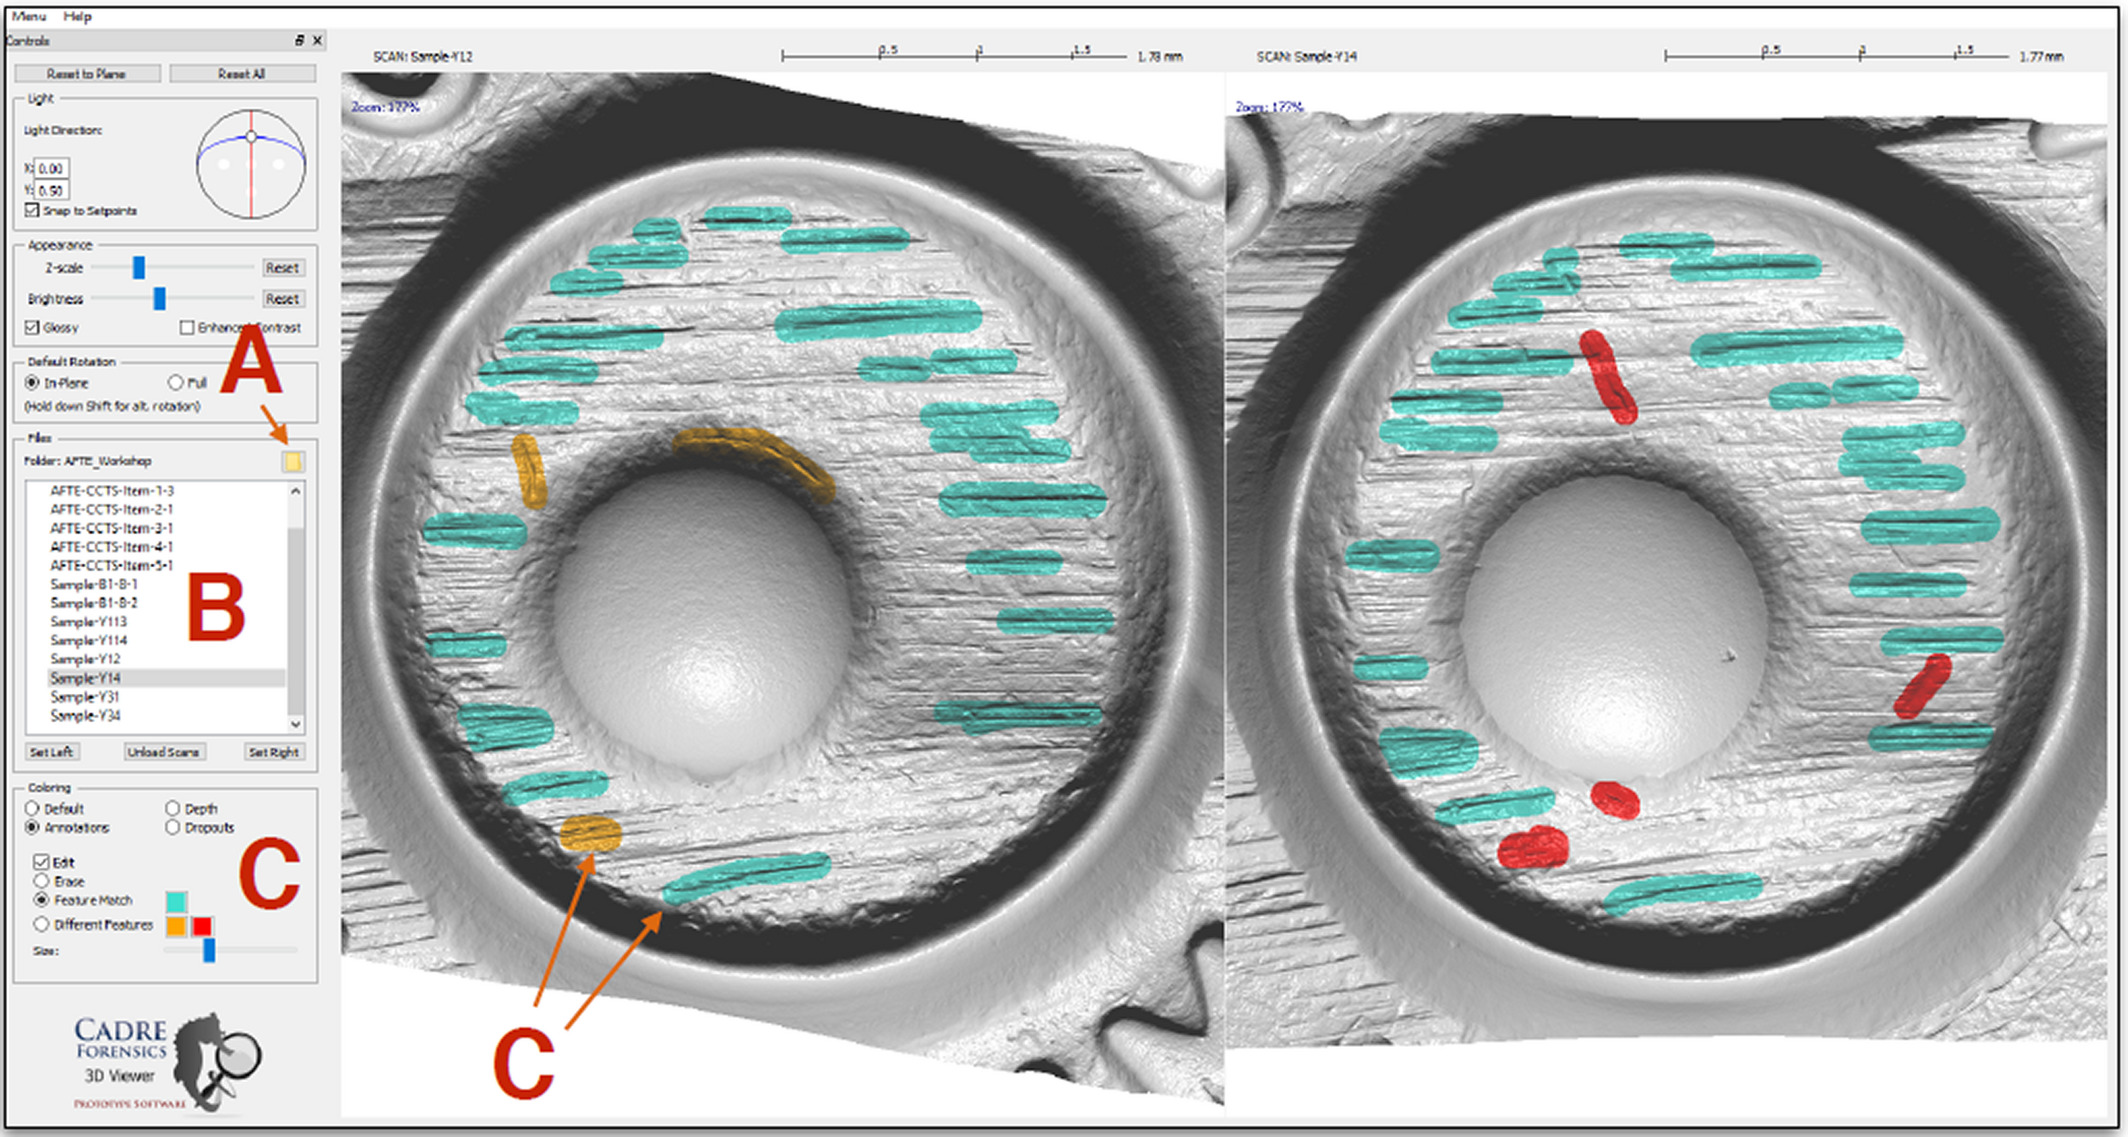
\includegraphics[width=\textwidth]{images/topMatchSoftwareAnnotation} 

}

\caption{A screenshot of the TopMatch-3D\texttrademark\ Virtual Comparison Microscopy software. In this example, similar and different markings on the cartridge case scans are manually annotated by the user using shades of blue and yellow/red, respectively.}\label{fig:topMatchAnnotationExample}
\end{figure}

In Chapter 3, we introduce a suite of static and interactive visual diagnostic tools.
We discuss how these visual diagnostic tools can be used by both researchers and practitioners to understand the behavior of automatic cartridge case comparison algorithms.

\hypertarget{automating-and-improving-the-cartridge-case-comparison-pipeline}{%
\section{Automating and Improving the Cartridge Case Comparison Pipeline}\label{automating-and-improving-the-cartridge-case-comparison-pipeline}}

In this section, we review preliminaries needed to understand various sub-routines of the cartridge case comparison pipeline.

\hypertarget{image-processing-techniques}{%
\subsection{Image Processing Techniques}\label{image-processing-techniques}}

We first review image processing and computer vision algorithms used in cartridge case comparison algorithms.
Throughout this section, let \(A, B \in \mathbb{R}^{k \times k}\) denote two images for \(k > 0\).
We use lowercase letters and subscripts to denote a particular value of a matrix: \(a_{ij}\) is the value in the \(i\)-th row and \(j\)-th column, starting in the top-left corner, of matrix \(A\).
In our application, \(A\) and \(B\) represent the surface matrices of two cartridge cases.

\hypertarget{image-registration}{%
\subsubsection{Image Registration}\label{image-registration}}

\emph{Image registration} involves transforming image \(B\) to align best with image \(A\) (or vice versa) \citep{Brown1992}.
In our application, this transformation is composed of a discrete translation \((m^*,n^*) \in \mathbb{Z}^2\) and rotation by \(\theta^* \in [-180^\circ, 180^\circ]\).
Together, we refer to \((m^*,n^*,\theta^*)\) as the ``registration'' of image \(B\) to \(A\).
To determine the optimal registration, we calculate the \emph{cross-correlation function} between \(A\) and \(B\), denoted \((A \star B)\), which measures the similarity between \(A\) and \(B\) for every possible translation of \(B\).
The CCF between \(A\) and \(B\) is a 2D array of dimension \(2k - 1 \times 2k - 1\) where the value of the \(m,n\)-th element is given by:
\[
(a \star b)_{mn} = \sum_{i=1}^k \sum_{j=1}^k a_{mn} \cdot b_{i + m,j + n}
\]
where \(1 \leq m,n \leq 2k -1\).
The value \((a \star b)_{mn}\) quantifies the similarity between \(A\) and \(B\) after \(B\) is translated \(m\) elements horizontally and \(n\) elements vertically.

A natural choice for aligning \(A\) and \(B\) is the translation that maximizes the CCF.
However, we must also consider that \(B\) may also need to be rotated to align optimally with \(A\).
We therefore compute the maximum CCF value across a range of rotations of \(B\).
Let \(B_\theta\) denote \(B\) rotated by an angle \(\theta\) and \(b_{\theta_{mn}}\) the \(m,n\)-th element of \(B_\theta\). Then the estimated registration \((m^*, n^*, \theta^*)\) is:
\[
(m^*, n^*, \theta^*) = \arg \max_{m,n,\theta} (a \star b_{\theta})_{mn}.
\]

In practice, we consider a discrete range of rotations \(\Theta \subset [-180^\circ, 180^\circ]\).
The registration procedure is given by:

\begin{enumerate}
\def\labelenumi{\arabic{enumi}.}
\tightlist
\item
  For each \(\theta \in \pmb{\Theta}\):
\end{enumerate}

\begin{quote}
1.1 Rotate image \(B\) by \(\theta\) to obtain \(B_\theta\).
\end{quote}

\begin{quote}
1.2 Calculate the CCF between \(A\) and \(B_\theta\).
\end{quote}

\begin{quote}
1.3 Determine the translation \([m_{\theta}^*,n_{\theta}^*]\) at which the CCF is maximized. Also, record the CCF value associated with this translation.
\end{quote}

\begin{enumerate}
\def\labelenumi{\arabic{enumi}.}
\setcounter{enumi}{1}
\item
  Across all \(\theta \in \Theta\), determine the rotation \(\theta^*\) at which the largest CCF value is achieved.
\item
  The estimated registration consists of rotation \(\theta^*\) and translation \([m^*,n^*] \equiv [m_{\theta^*}^*,n_{\theta^*}^*]\).
\end{enumerate}

In this instance, we refer to image \(A\) as the ``reference'' and \(B\), the image aligned to the reference, as the ``target.''
We represent the transformation to register \(B\) to \(A\) element-wise where the index \(i,j\) maps to \(i^*,j^*\) by:
\[
\begin{pmatrix} j^* \\ i^* \end{pmatrix} = \begin{pmatrix} n^* \\ m^* \end{pmatrix} + \begin{pmatrix} \cos(\theta^*) & -\sin(\theta^*) \\ \sin(\theta^*) & \cos(\theta^*) \end{pmatrix} \begin{pmatrix} j \\ i \end{pmatrix}.
\]
Under this transformation, the value \(b_{ij}\) now occupies the the \(i^*,j^*\)-th element.
In practice, we use \emph{nearest-neighbor interpolation} meaning \(i^*\) and \(j^*\) are rounded to the nearest integer.

Based on the definition given above, the CCF is computationally taxing.
In image processing, it is common to use an implementation based on the Fast Fourier Transform \citep{Brown1992}.
This implementation leverages the Cross-Correlation Theorem, which states that for images \(A\) and \(B\) the CCF can be expressed in terms of a frequency-domain pointwise product:
\[
(A \star B)[m,n] = \mathcal{F}^{-1}\left(\overline{\mathcal{F}(A)} \odot \mathcal{F}(B)\right)[m,n]
\]
where \(\mathcal{F}\) and \(\mathcal{F}^{-1}\) denote the discrete Fourier and inverse discrete Fourier transforms, respectively, and \(\overline{\mathcal{F}(A)}\) denotes the complex conjugate \citep{fft_brigham}.
Because the product on the right-hand side is calculated pointwise, this result allows us to trade the moving sum computations from the definition of the CCF for two forward Fourier transformations, a pointwise product, and an inverse Fourier transformation.
The Fast Fourier Transform (FFT) algorithm can be used to reduce the computational load considerably.

Figure \ref{fig:ccfTranslationExample} shows an example of two images \(A\) and \(B\) of dimension \(100 \times 100\) and \(21 \times 21\), respectively.
The white boxes in both of the images are of dimension \(10 \times 10\).
The box in image A is centered on index {[}30,50{]} while the box in image B is centered on index {[}11,11{]}.
The right image shows the result of calculating the CCF using image \(A\) as reference and \(B\) as template.
The CCF achieves a maximum of 1, indicating a perfect match, at the translation value of \([m^*,n^*] = [22,-2]\).
This means that if image B were overlaid onto image A such that their center indices coincided, then image B would need to be shifted 22 units ``up'' and 2 units ``left'' to match perfectly with image A.

\begin{figure}[!htbp]

{\centering 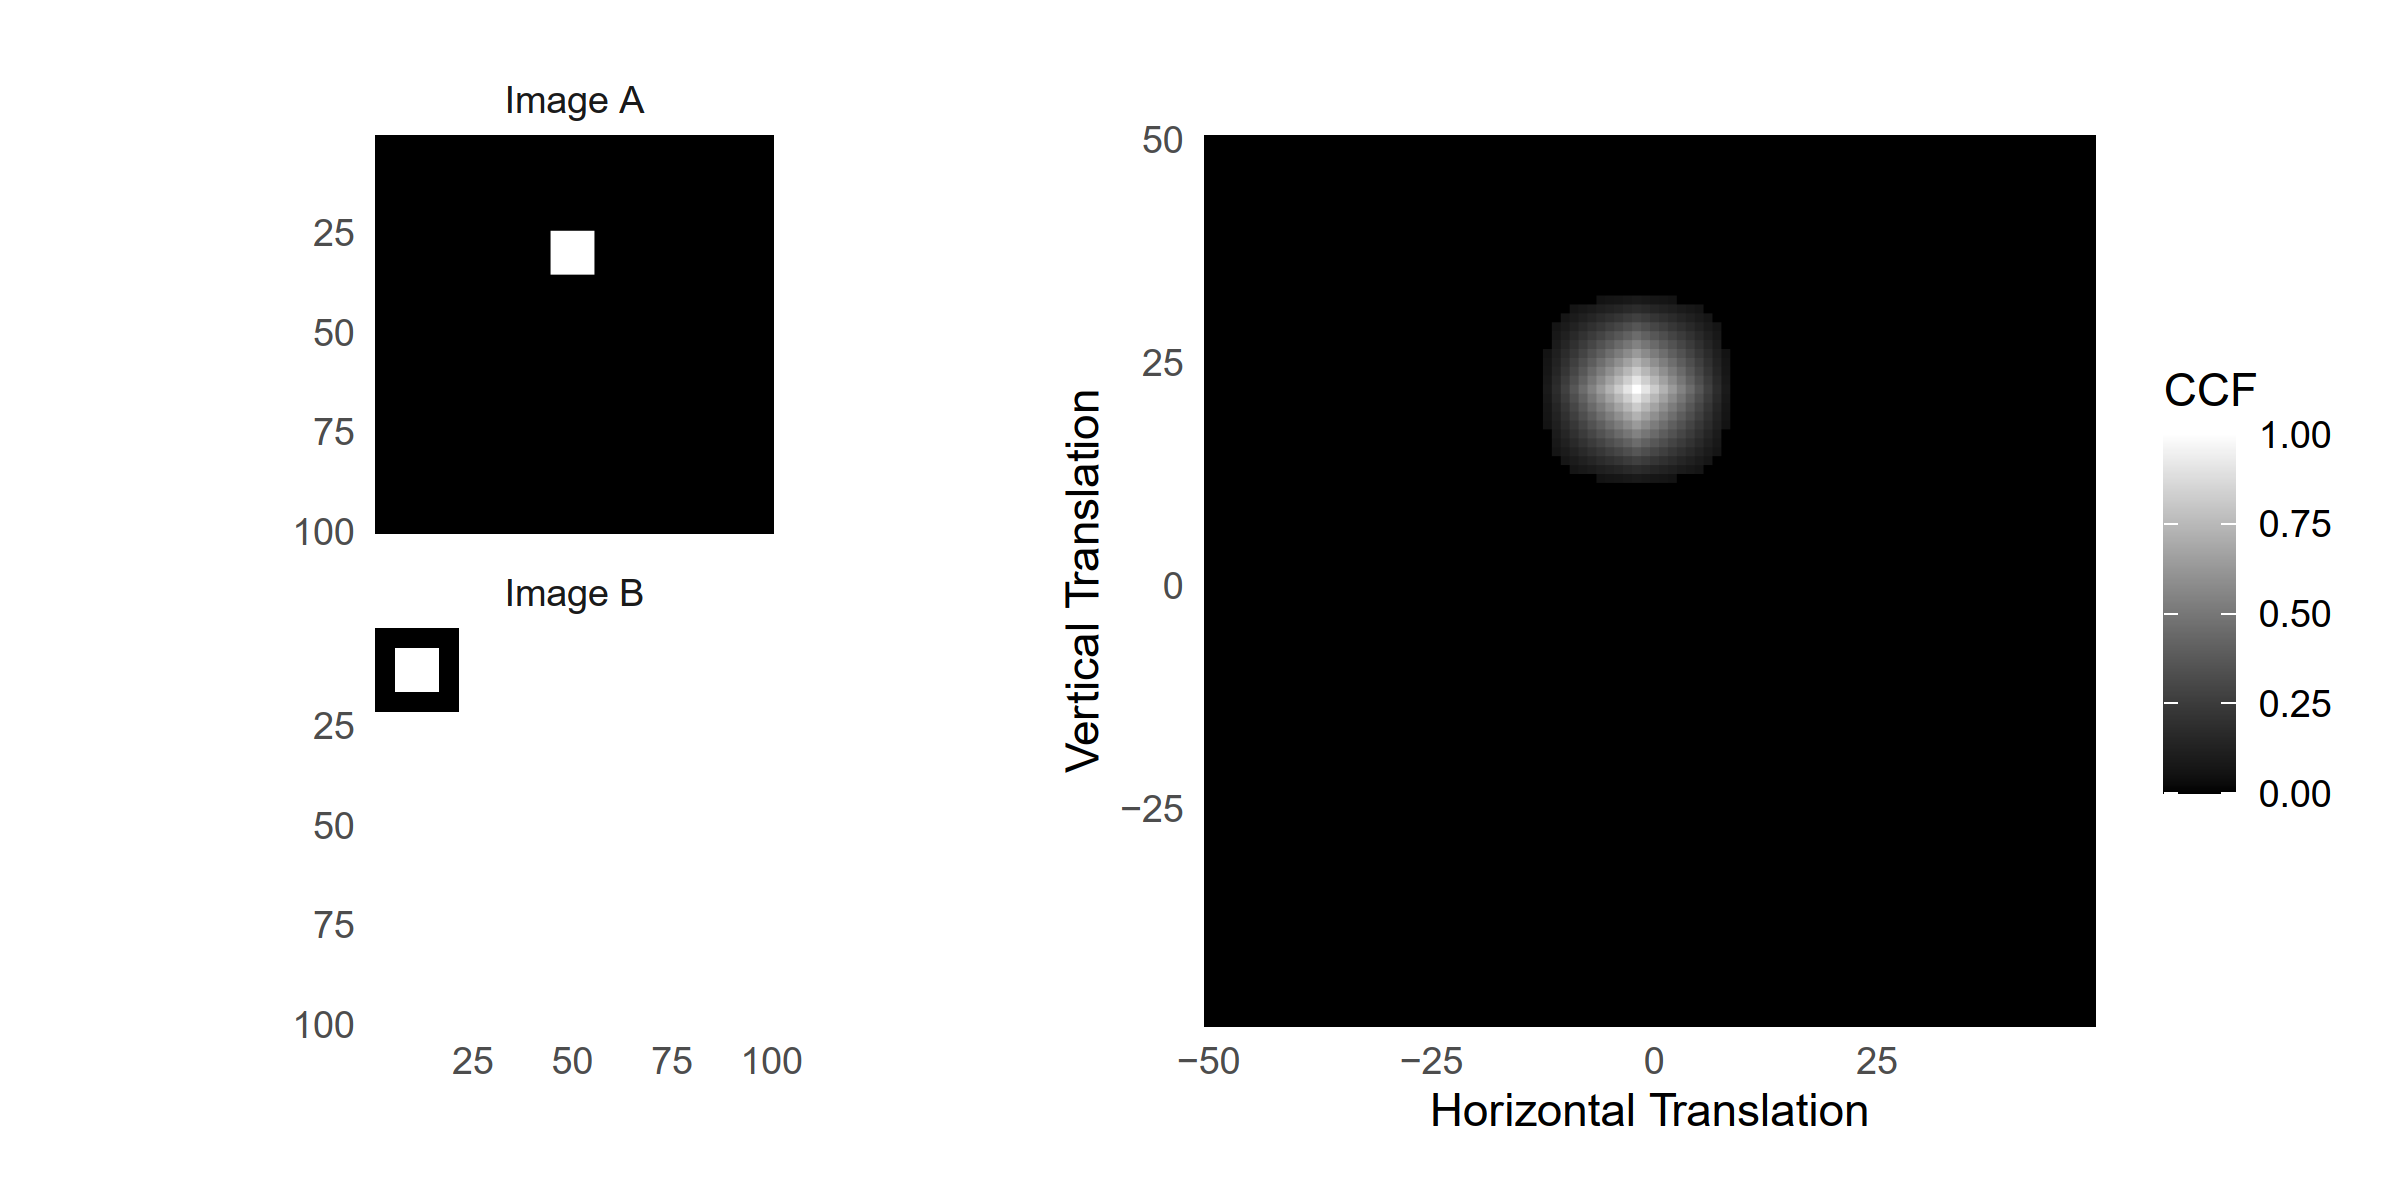
\includegraphics[width=\textwidth]{figures/unnamed-chunk-13-1} 

}

\caption{(Left) A reference image $A$ and template image $B$ both featuring a white box of dimension $10 \times 10$. (Right) The cross-correlation function (CCF) between $A$ and $B$. The index at which the CCF is maximized represents the translation at which $A$ and $B$ are most similar.}\label{fig:ccfTranslationExample}
\end{figure}

\hypertarget{gaussian-filters}{%
\subsubsection{Gaussian Filters}\label{gaussian-filters}}

In image processing, a Gaussian filter (equivalently, blur or smoother) is a mathematical operator that imputes the values in an image using a locally-weighted sum of surrounding values.
We use a \emph{lowpass} Gaussian filter to smooth the surface values of a cartridge case scan.
The weights are dictated according to the Gaussian function of a chosen standard deviation \(\sigma\) given by:

\[
f(n,m;\sigma) = \frac{1}{2\pi\sigma^2} \exp\left(-\frac{1}{2\sigma^2}(n^2 + m^2)\right).
\]
It is common to populate a 2D array with the values of the Gaussian function treating the center index as the origin.
Such an array is called a \emph{kernel}.
An example of a \(3 \times 3\) Gaussian kernel \(K\) with standard deviation \(\sigma = 1\) is given below.
\[
K = 
\begin{pmatrix}
0.075 & 0.124 & 0.075 \\
0.124 & 0.204 & 0.124 \\
0.075 & 0.124 & 0.075
\end{pmatrix}.
\]

For an image \(A\) and Gaussian kernel \(K\) with standard deviation \(\sigma\), the lowpass filtered version of \(A\), denoted \(A_{lp,\sigma}\) is given by:
\[
A_{lp,\sigma}[m,n] = \mathcal{F}^{-1}\left(\mathcal{F}(A) \odot \mathcal{F}(K)\right)[m,n].
\]
This operation, known as \emph{convolution}, is extremely similar to the calculation of the CCF defined in the Image Registration section \citep{ISO1661021}.

From left to right, Figure \ref{fig:gaussianFilterExample} shows an image \(A\) of a box injected with Gaussian noise (noise standard deviation \(\sigma_n = 0.3\)) followed by the application of various Gaussian filters.
In the middle of Figure \ref{fig:gaussianFilterExample}, we see that the lowpass filter (kernel standard deviation \(\sigma_k = 2\)) recovers some of the definition of the box by ``smoothing'' some of the Gaussian noise.

If a lowpass filter smooths values in an image, then a \emph{highpass} filter performs a ``sharpening'' operation.
For an image \(A\) and kernel standard deviation \(\sigma\), the highpass filtered version \(A_{hp}\) can be defined as:
\begin{align*}
A_{hp,\sigma} = A - A_{lp,\sigma}.
\end{align*}
The highpass filter therefore removes larger-scale (smooth) structure from an image and retains high-frequency structure such as noise or edges.
The fourth facet of Figure \ref{fig:gaussianFilterExample} shows a highpass-filtered image \(A\) .
The smooth interior of the box is effectively removed from the image while the edges are preserved.

Finally, a \emph{bandpass} Gaussian filter simultaneously performs highpass sharpening and lowpass smoothing operations.
Generally, the standard deviation of the highpass kernel will be considerably larger than that of the lowpass kernel.
This leads to retaining sharp edges while also reducing noise.
An example of a bandpass filtered image \(A\) is shown in Figure \ref{fig:gaussianFilterExample}.
The edges of the box are better-preserved compared to the lowpass filter figure while the interior of the box is better-preserved compared to the highpass filter figure.

\begin{figure}[!htbp]

{\centering 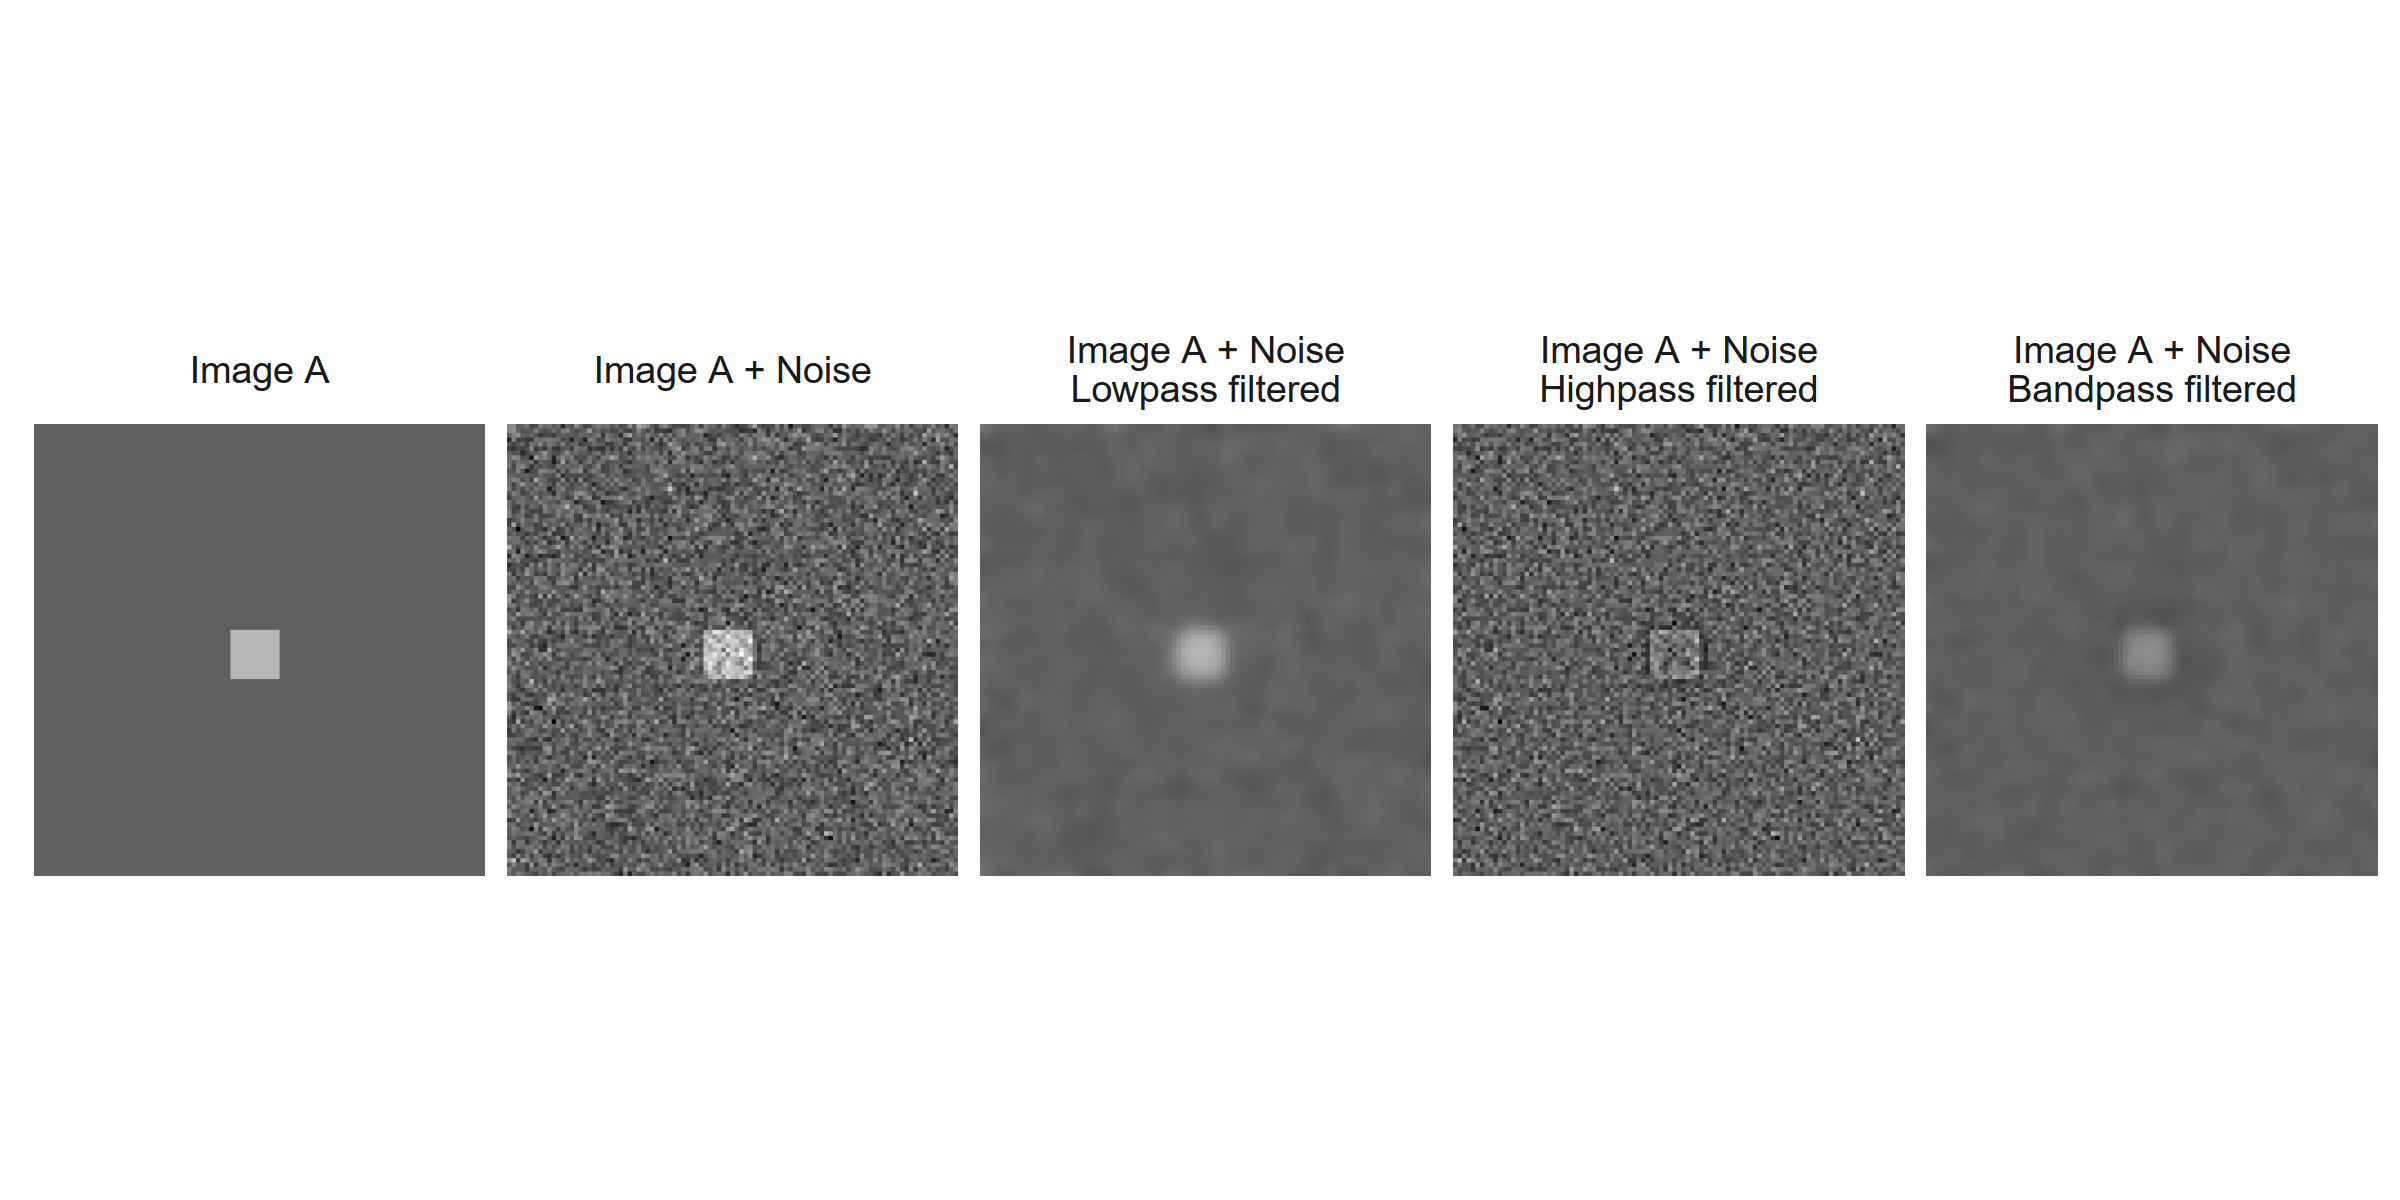
\includegraphics[width=\textwidth]{figures/unnamed-chunk-14-1} 

}

\caption{An image $A$ of a box with Gaussian noise undergoing a lowpass, highpass, and bandpass filter operation.}\label{fig:gaussianFilterExample}
\end{figure}

Variations on the standard Gaussian filter include the ``robust'' Gaussian regression filter.
This filter fluctuates between a filter step, which applies a Gaussian filter, and outlier step, which identifies and omits outlier observations from the next filter step \citep{robustFilter}.
Another alternative, the ``edge preserving'' filter, adapts the kernel weights when approaching the boundary of an image to mitigate so-called \emph{boundary effects} \citep{Aurich1995}.

We use Gaussian filters to change the values on the interior of a cartridge case surface to better emphasize breech face impressions.
In the next section, we discuss applying morphological operations to change the values on the edges of a cartridge case surface.

\hypertarget{morphological-operations}{%
\subsubsection{Morphological Operations}\label{morphological-operations}}

Mathematical morphology refers to a theory and collection of image processing techniques for geometrical structures \citep{Haralick1987}.
In our application, these geometrical structures are cartridge case scans; specifically, binarized versions of these scans representing whether a particular pixel contains part of the cartridge case surface.
We discuss this in greater detail in Chapter 2.

Two fundamental operations in mathematical morphology are \emph{dilation} and \emph{erosion} \citep{Haralick1987}.
For our purposes, these are both set operations on black and white, encoded as 0 and 1 respectively, images.
We call the set of black and white pixels the ``background'' and ``foreground'' of the image, respectively.
For an image \(A\), let \(W = \{(m,n) : A_{mn} = 1\}\) denote the foreground of \(A\).
An example of a \(7 \times 7\) binary image \(A\) with \(W = \{(3,3),(3,4),(3,5),(4,3),(4,4),(4,5),(5,3),(5,4),(5,5)\}\) is given below.
\[
A = 
\begin{pmatrix}
0 & 0 & 0 & 0 & 0 & 0 & 0 \\
0 & 0 & 0 & 0 & 0 & 0 & 0 \\
0 & 0 & 1 & 1 & 1 & 0 & 0 \\
0 & 0 & 1 & 1 & 1 & 0 & 0 \\
0 & 0 & 1 & 1 & 1 & 0 & 0 \\
0 & 0 & 0 & 0 & 0 & 0 & 0 \\
0 & 0 & 0 & 0 & 0 & 0 & 0
\end{pmatrix}
\]

A \emph{structuring element} is a second, typically small, array \(B\) of ones that affects the amount of dilation or erosion applied to \(W\) within \(A\).
For simplicity, the indexing of the structuring element uses the center element as the index origin.
For example, a \(3 \times 3\) structuring element is given by \(B = \{(-1,-1),(-1,0),(-1,1),(-1,0),(0,0),(0,1),(1,-1),(1,0),(1,1)\}\) or visually:
\[
B = 
\begin{pmatrix}
1 & 1 & 1 \\
1 & 1 & 1 \\
1 & 1 & 1 
\end{pmatrix}
\]

As the name suggests, a \emph{dilation} grows the region \(W\) within image \(A\) by replacing 0-valued pixels that border \(W\) with 1.
The structuring element \(B\) dictates which pixels are replaced with 1.
We define the dilation of \(W\) by \(B\), denoted \(W \oplus B\), element-wise:
\[
W \oplus B = \{[m,n] \in A : [m,n] = [i + k,j + l] \text{ for } [i,j] \in W \text{ and } [k,l] \in B\}
\]

In our example,
\[W \oplus B = \{[3,2],[3,3],[3,4],[3,5],[3,6],[4,2],[4,3],[4,4],[4,5],[4,6],[5,2],[5,3],[5,4],[5,5],[5,6]\}\]
or visually:
\[
W \oplus B = 
\begin{pmatrix}
0 & 0 & 0 & 0 & 0 & 0 & 0 \\
0 & 1 & 1 & 1 & 1 & 1 & 0 \\
0 & 1 & 1 & 1 & 1 & 1 & 0 \\
0 & 1 & 1 & 1 & 1 & 1 & 0 \\
0 & 1 & 1 & 1 & 1 & 1 & 0 \\
0 & 1 & 1 & 1 & 1 & 1 & 0 \\
0 & 0 & 0 & 0 & 0 & 0 & 0
\end{pmatrix}.
\]
The dilation operation by this \(B\) has the effect of growing the region \(W\) inside of \(A\) by one index in each direction.

In contrast, \emph{erosion} has the effect of shrinking \(W\).
The erosion of \(W\) by \(B\) is:
\[
A \ominus B = \{[m,n] \in A: [m,n] + [k,l] \in A \text{ for every } [k,l] \in B\}.
\]

Using the same example as above, \(W \ominus B = \{[3,3]\}\) or visually:
\[
W \ominus B =
\begin{pmatrix}
0 & 0 & 0 & 0 & 0 & 0 & 0 \\
0 & 0 & 0 & 0 & 0 & 0 & 0 \\
0 & 0 & 0 & 0 & 0 & 0 & 0 \\
0 & 0 & 0 & 1 & 0 & 0 & 0 \\
0 & 0 & 0 & 0 & 0 & 0 & 0 \\
0 & 0 & 0 & 0 & 0 & 0 & 0 \\
0 & 0 & 0 & 0 & 0 & 0 & 0
\end{pmatrix}.
\]
Erosion by this \(B\) shrinks the region \(W\) in \(A\) by one index in each direction.

Figure \ref{fig:dilationErosionExample} shows our example represented using black and white pixels.
In practice, the foreground set \(W\) may contain disconnected regions to which dilation or erosion can be independently applied.

\begin{figure}[!htbp]

{\centering 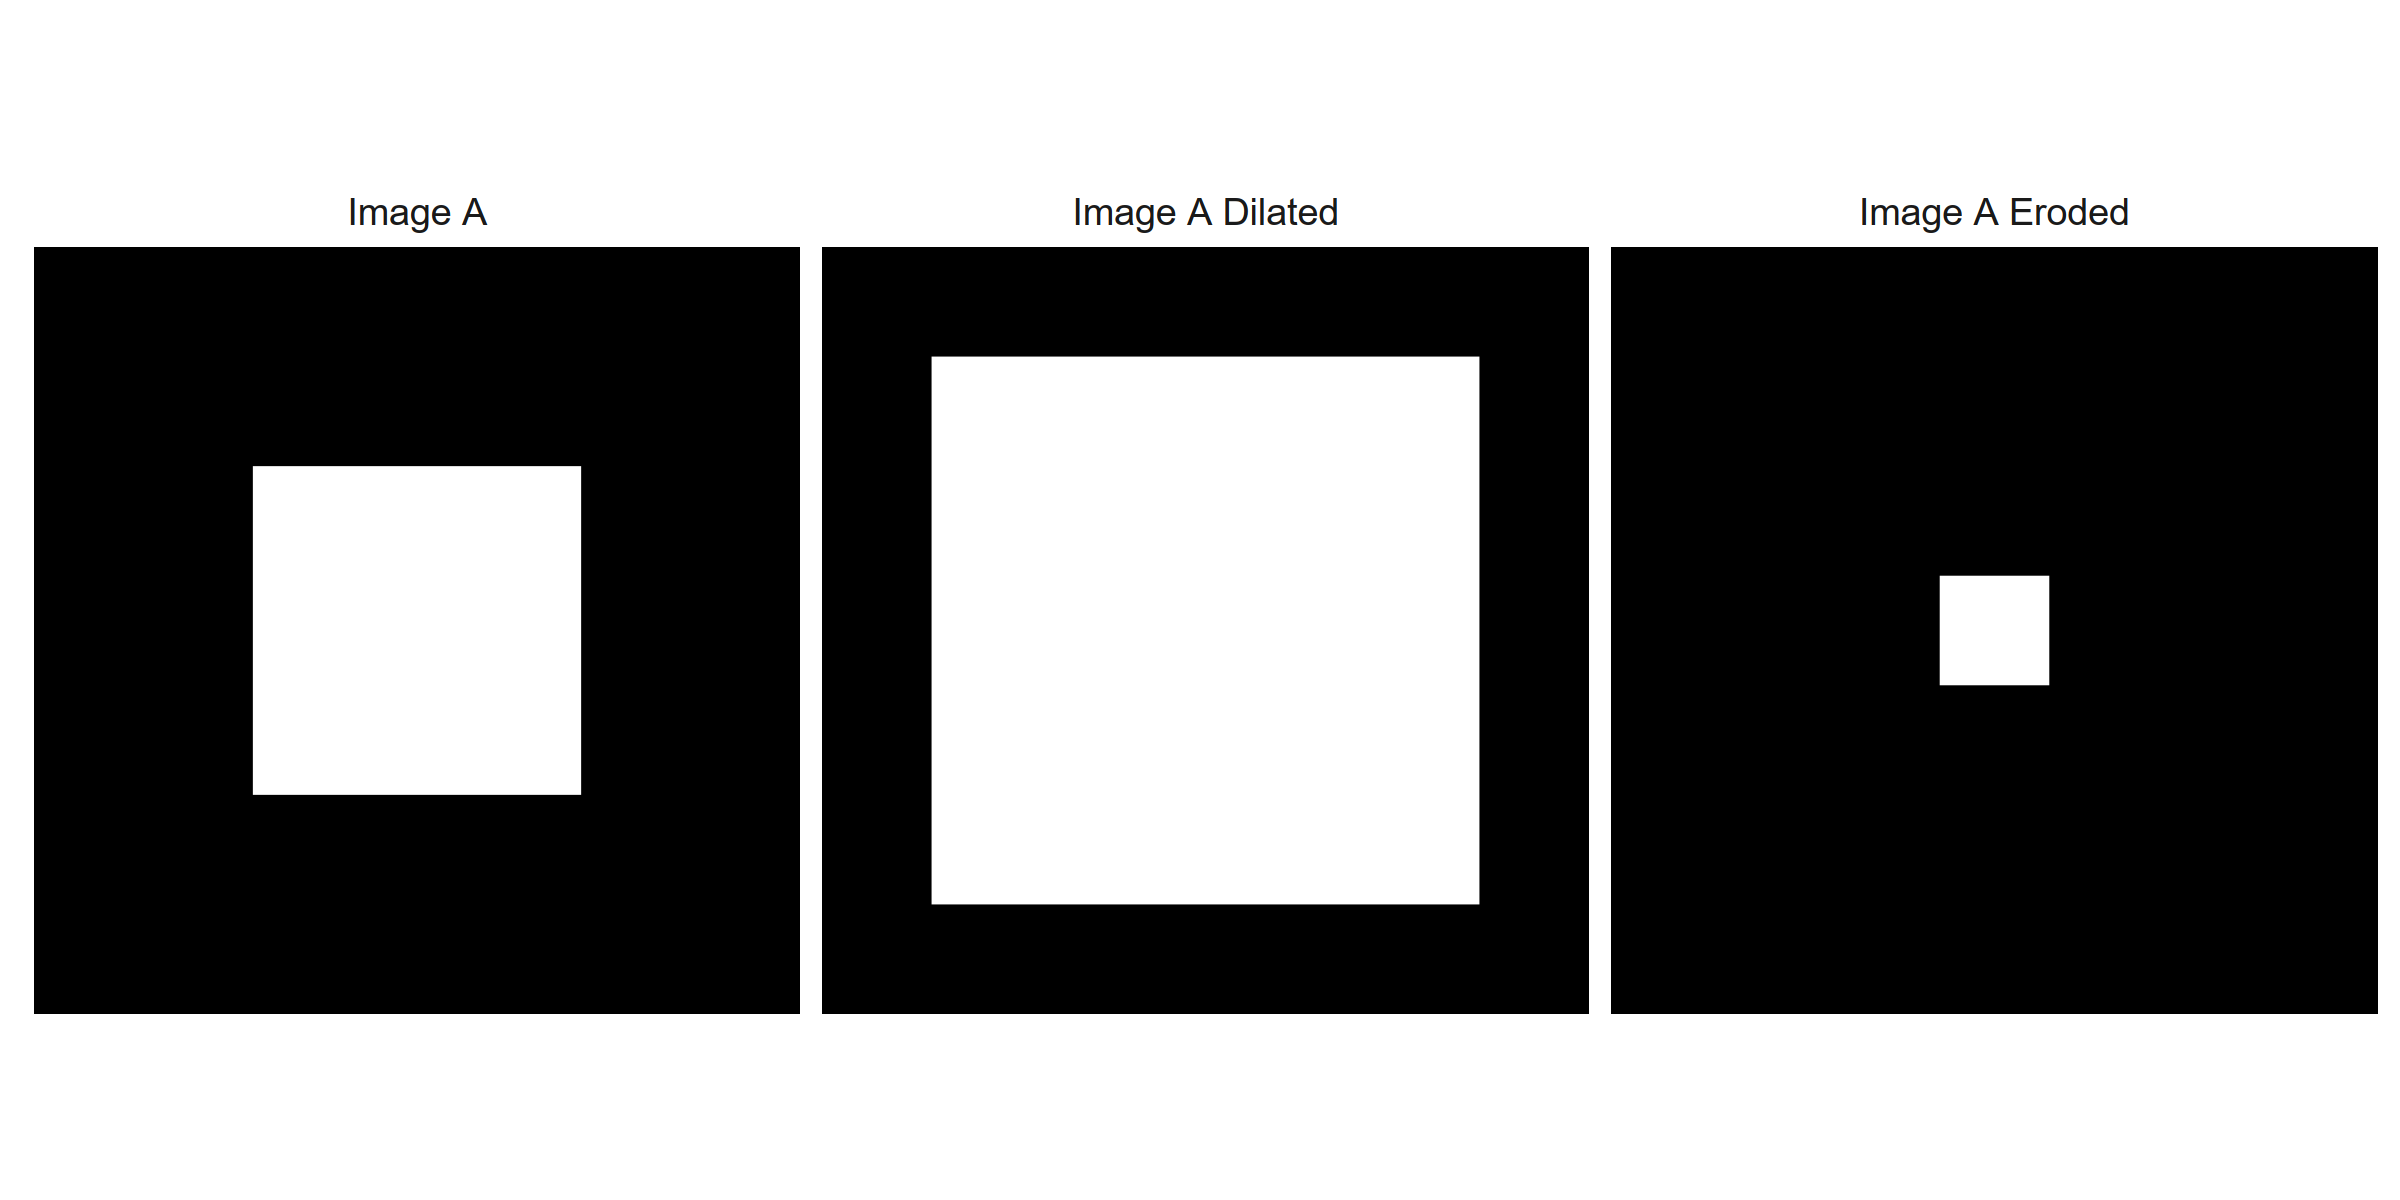
\includegraphics[width=\textwidth]{figures/unnamed-chunk-15-1} 

}

\caption{A $7 \times 7$ image $A$ featuring a $3 \times 3$ box undergoing dilation and erosion by a $3 \times 3$ structuring element $B$.}\label{fig:dilationErosionExample}
\end{figure}

This concludes our review of image processing techniques we use in subsequent chapters.
Next, we discuss a clustering procedure used in Chapter 4 to calculate similarity features.

\hypertarget{density-based-spatial-clustering-of-applications-with-noise}{%
\subsection{Density-Based Spatial Clustering of Applications with Noise}\label{density-based-spatial-clustering-of-applications-with-noise}}

The Density-Based Spatial Clustering of Applications with Noise (DBSCAN) algorithm is a clustering procedure that assigns observations to clusters if they are in a region of high observation density \citep{Ester1996}.
As we will see, the DBSCAN algorithm does not require the user to pre-specify the number of expected clusters as is required in common clustering algorithms like K-means.
Further, the algorithm does not require that all points be assigned to a cluster.

Let \(D\) represent a \(n \times p\) data set (\(n\) observations, each of dimension \(p\)) and let \(x,y,z \in D\) denote three observations.
The DBSCAN algorithm relies on the notion of \(\epsilon\)-neighborhoods.
Given some neighborhood radius \(\epsilon \in \mathbb{R}\) and distance metric \(d\), \(y\) is in the \(\epsilon\)-neighborhood of \(x\) if \(d(x,y) \leq \epsilon\).
The \emph{\(\epsilon\)-neighborhood} of \(x\) is defined as the set \(N_{\epsilon}(x) = \{y \in D : d(x,y) \leq \epsilon\}\).
Given a minimum number of points \(Minpts \in \mathbb{N}\) (notation used in \citep{Ester1996}), observation \(x\) is called a \emph{core point} with respect to \(\epsilon\) and \(Minpts\) if \(|N_{\epsilon}(x)| \geq Minpts\).
Core points are treated as the ``seeds'' of clusters in the DBSCAN algorithm.
The user must select values of \(\epsilon\) and \(Minpts\).

Figure \ref{fig:epsNeighborhoodExample} shows an example of a data set \(D \in \mathbb{R}^{10 \times 2}\).
We represent the 10 observations in \(D\) on the Cartesian plane.
An \(\epsilon\)-neighborhood using the Euclidean distance metric and \(\epsilon = 3\) is drawn around an observation \(x\) located at \((3,2)\).
Points inside the circle are neighbors of \(x\).
If, for example, \(Minpts = 2\), then \(x\) would be considered a core point.

\begin{figure}[!htbp]

{\centering 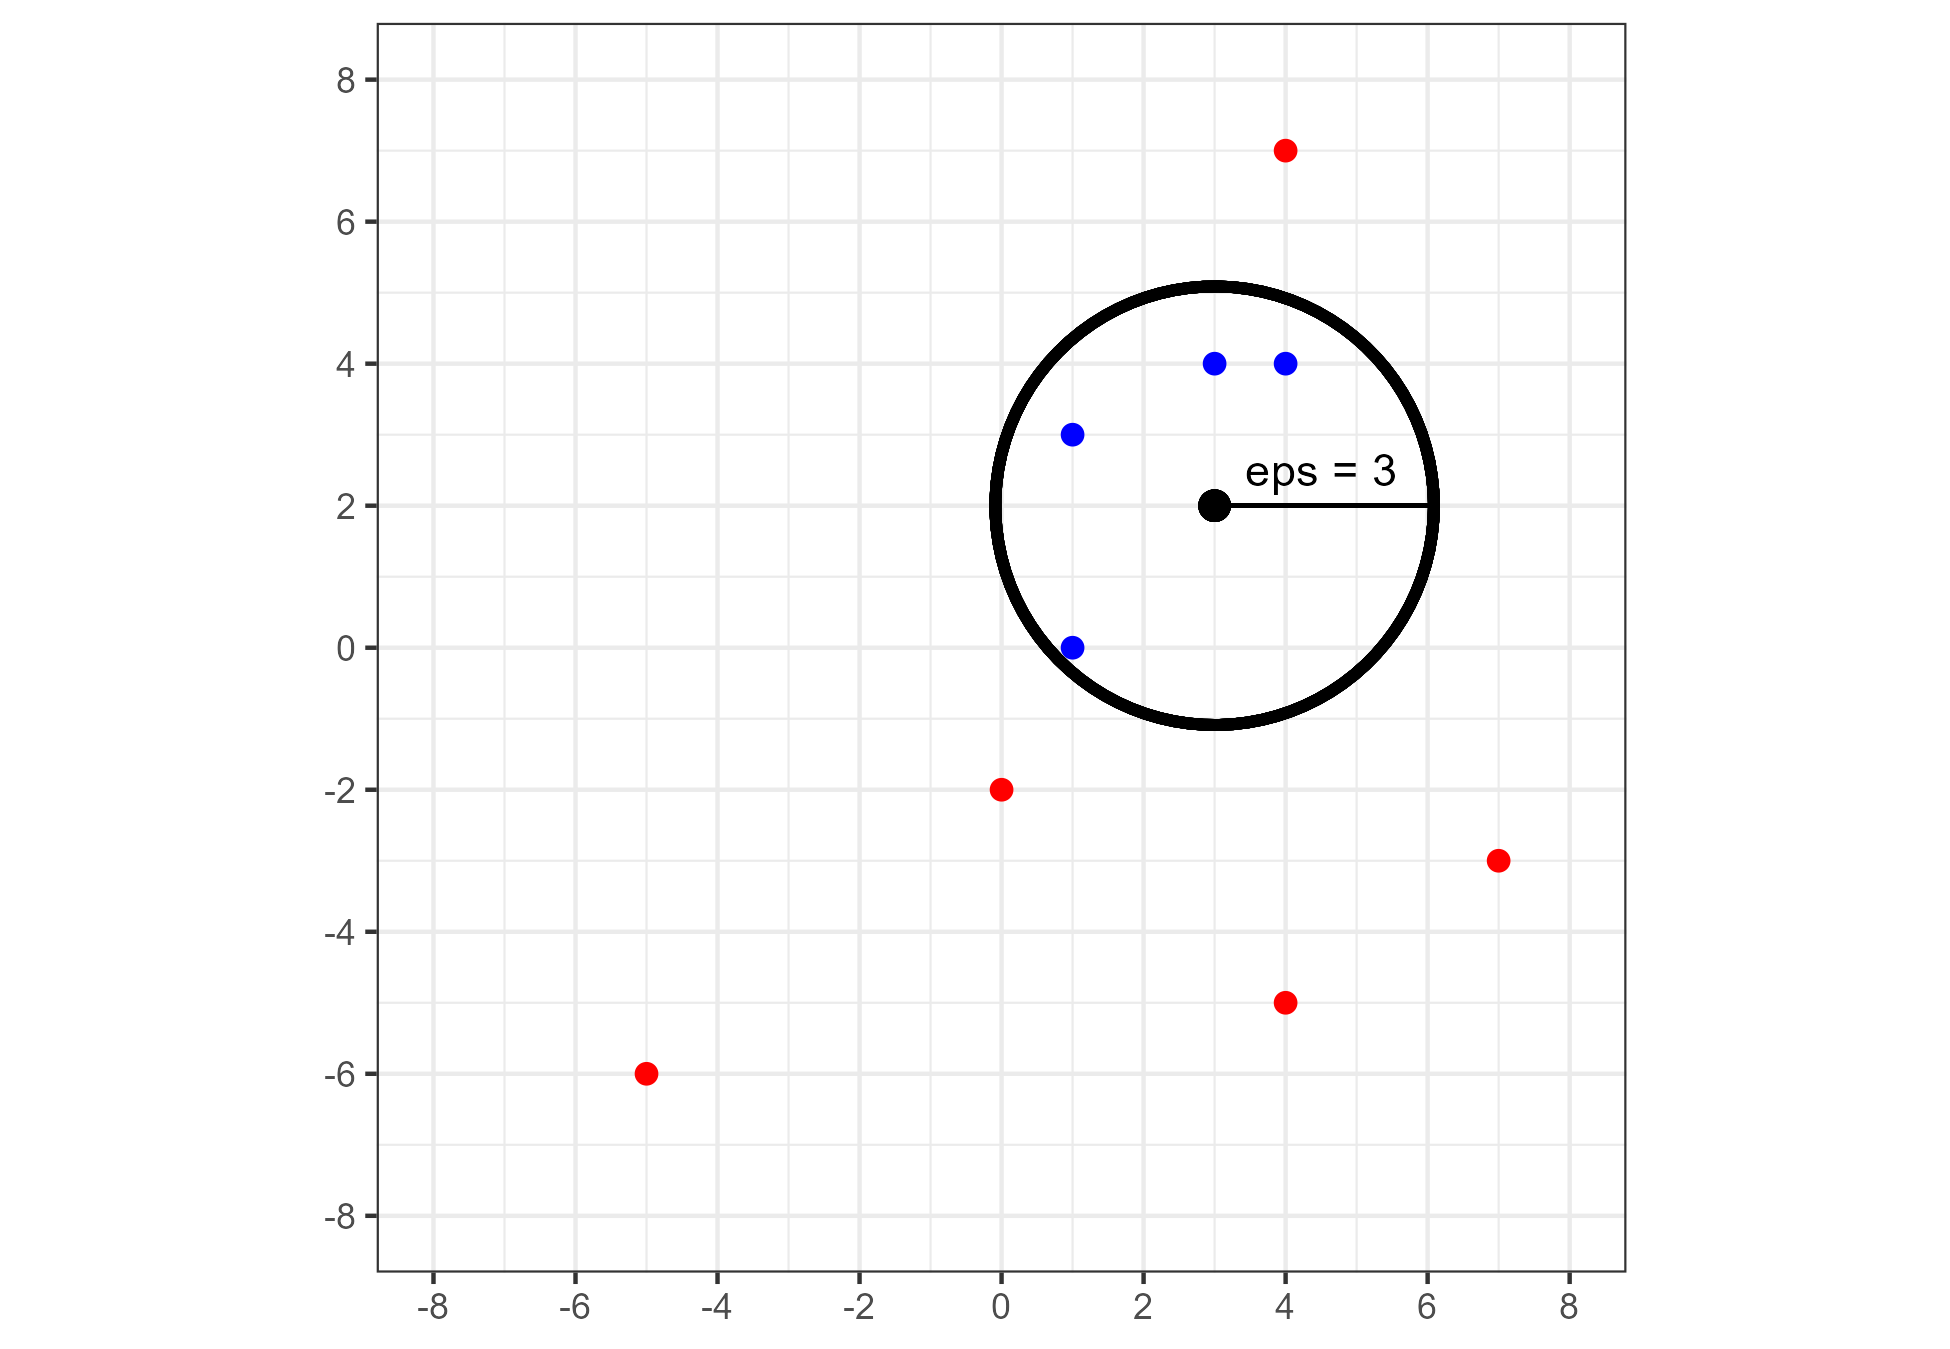
\includegraphics[width=.8\textwidth]{figures/dbscanExample_corePoint} 

}

\caption{An $\epsilon$-neighborhood around a observation located at $(3,2)$ for $\epsilon = 3$. Points are colored blue if they are neighbors to this observation and red otherwise.}\label{fig:epsNeighborhoodExample}
\end{figure}

\citep{Ester1996} introduces two relational notions, \emph{density-reachability} and \emph{density-connectivity}, to identify regions of high observation density.
A point \(y\) is \emph{directly density-reachable} to a point \(x\) if \(x\) is a core point and \(y \in N_{\epsilon}(x)\).
In Figure \ref{fig:epsNeighborhoodExample}, the observation located at \((1,0)\) is directly density-reachable to the observation located at \((3,2)\).
More broadly, a point \(x_m\) is \emph{density-reachable} to a point \(x_1\) if there exists a chain of observations \(x_1,x_2,...,x_{m-1},x_m\) such that \(x_{i+1}\) is directly density-reachable from \(x_i\), \(i = 1,...,n\).
Density reachability captures the notion of ``neighbors of neighbors'' for core points.
The DBSCAN algorithm agglomerates density-reachable points into single clusters.

Figure \ref{fig:densityReachableExample} highlights three points \((1,0), (3,2)\), and \((4,4)\).
Using \(\epsilon = 3\) and \(Minpts = 2\), we see that all three of these points are core points.
Further, the points at \((1,0)\) and \((4,4)\) are density-reachable by way of the point \((3,2)\).

\begin{figure}[!htbp]

{\centering 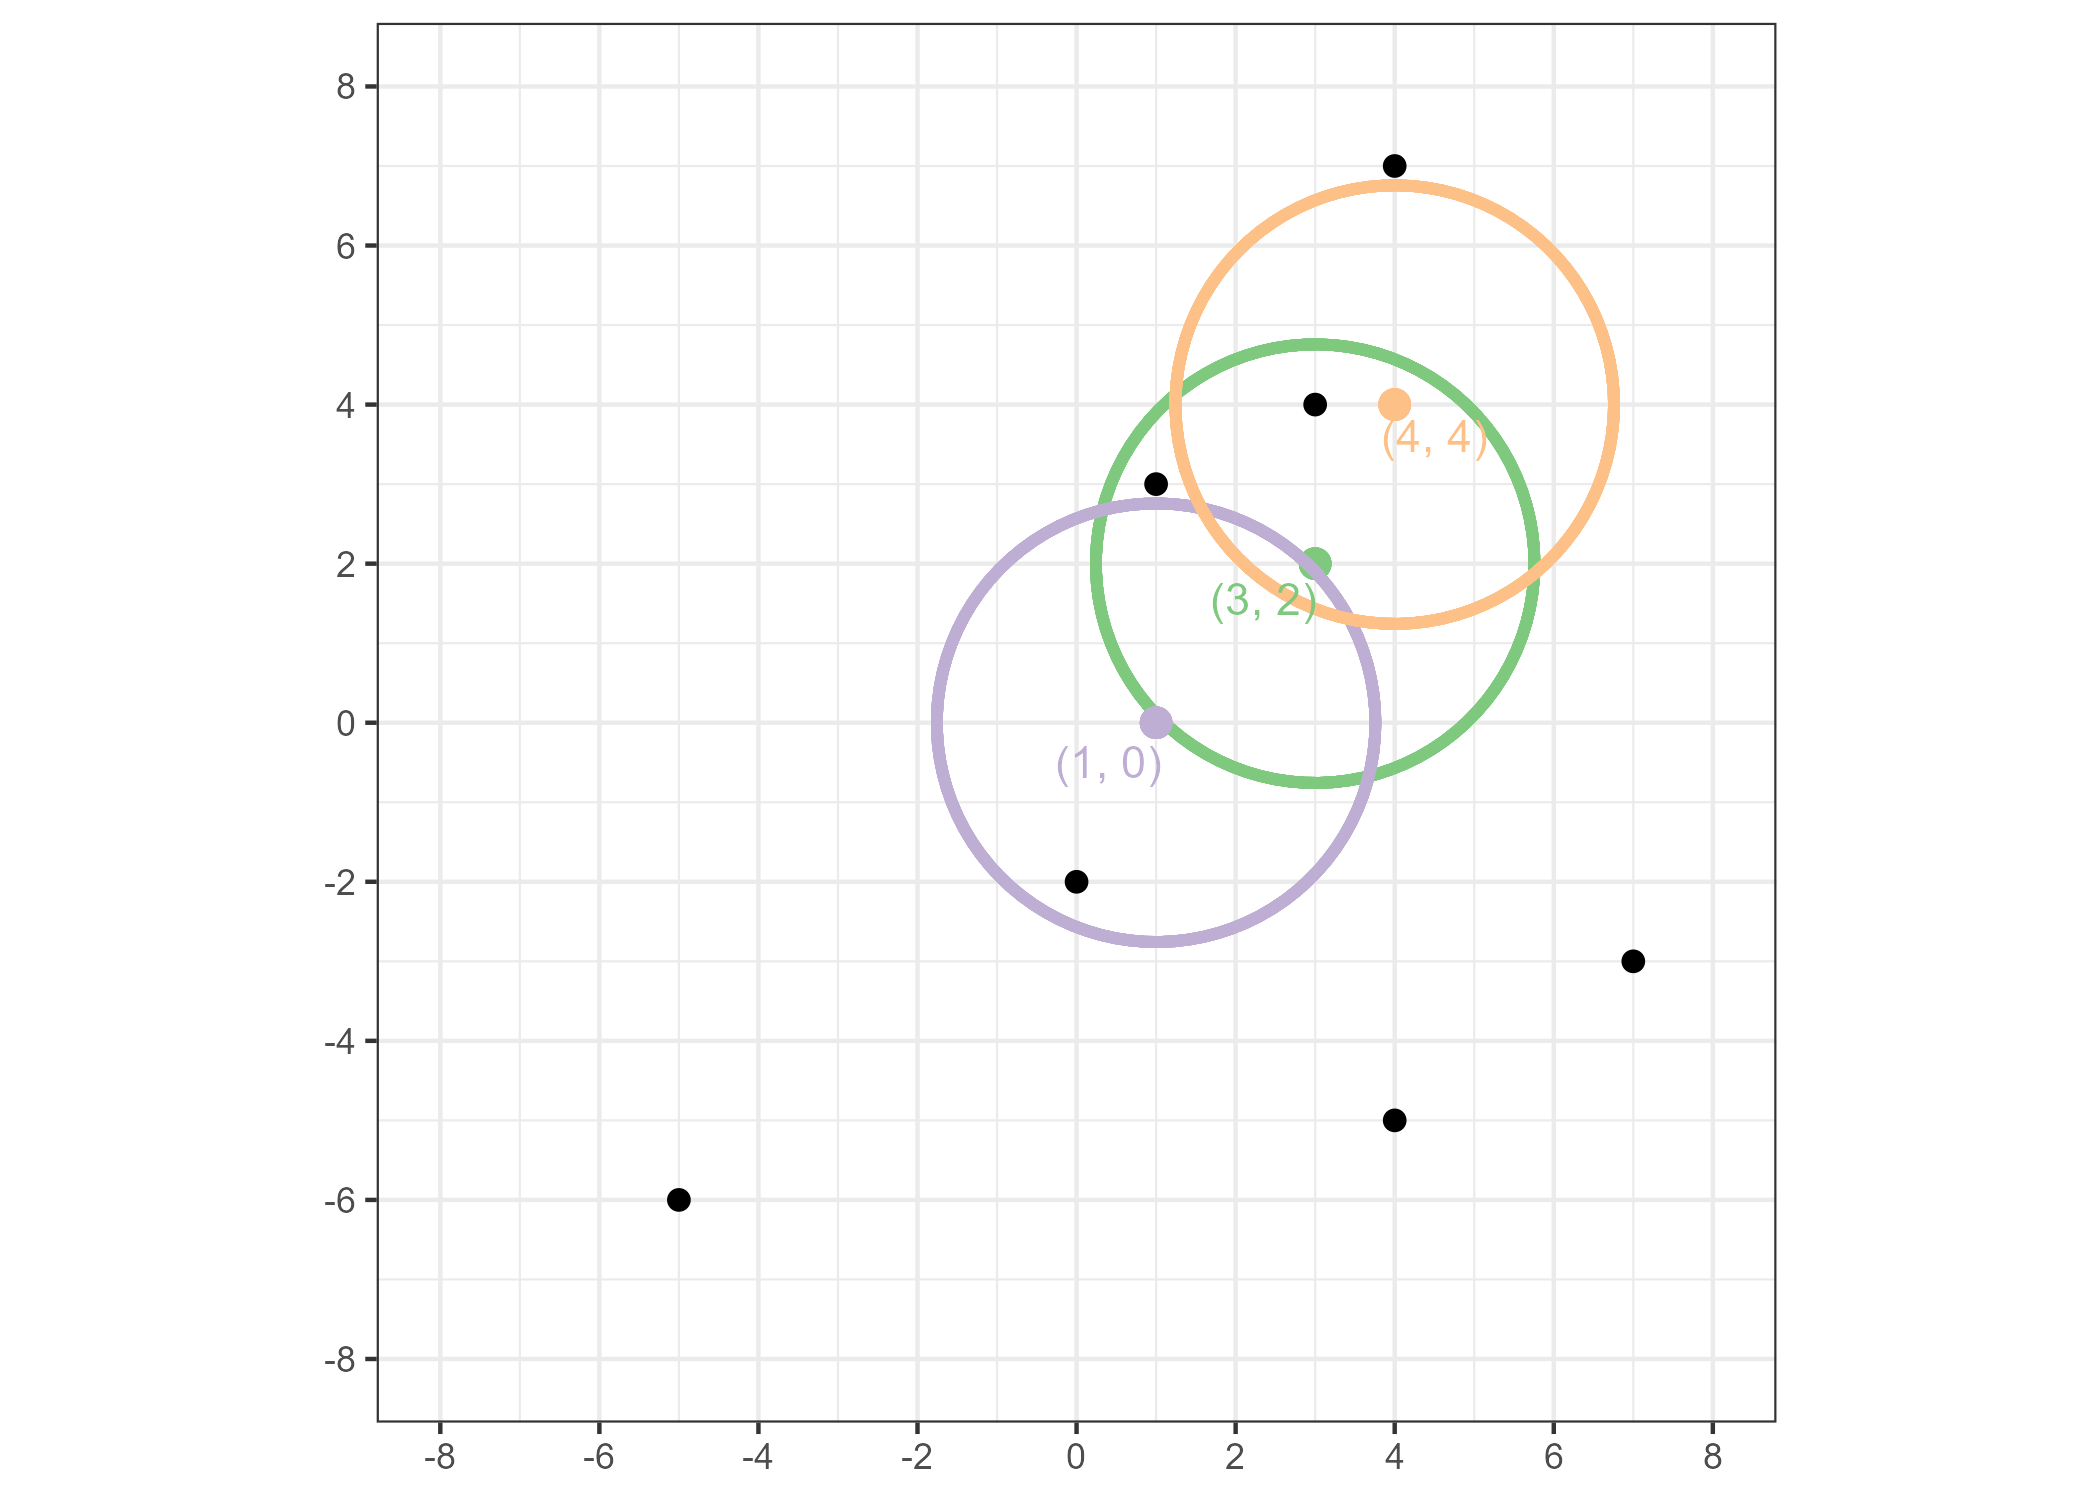
\includegraphics[width=.8\textwidth]{figures/dbscanExample_densityReachable} 

}

\caption{An example of three points that are density-reachable with respect to $\epsilon = 3$ and $Minpts = 2$.}\label{fig:densityReachableExample}
\end{figure}

Finally, a point \(y\) is \emph{density-connected} to a point \(x\) with respect to \(\epsilon\) and \(Minpts\) if there exists a point \(z\) such that both \(x\) and \(y\) are density-reachable to \(z\) (with respect to \(\epsilon\) and \(Minpts\)).
While density-reachability requires that all points in-between two points also be core points, density-connectivity extends the notion of ``neighbors of neighbors'' to include points that are merely within the neighborhood of density-reachable points.
Figure \ref{fig:densityConnectedExample} illustrates how the points located at \((4,7)\) and \((0,-2)\) are density-connected but not density-reachable.

\begin{figure}[!htbp]

{\centering 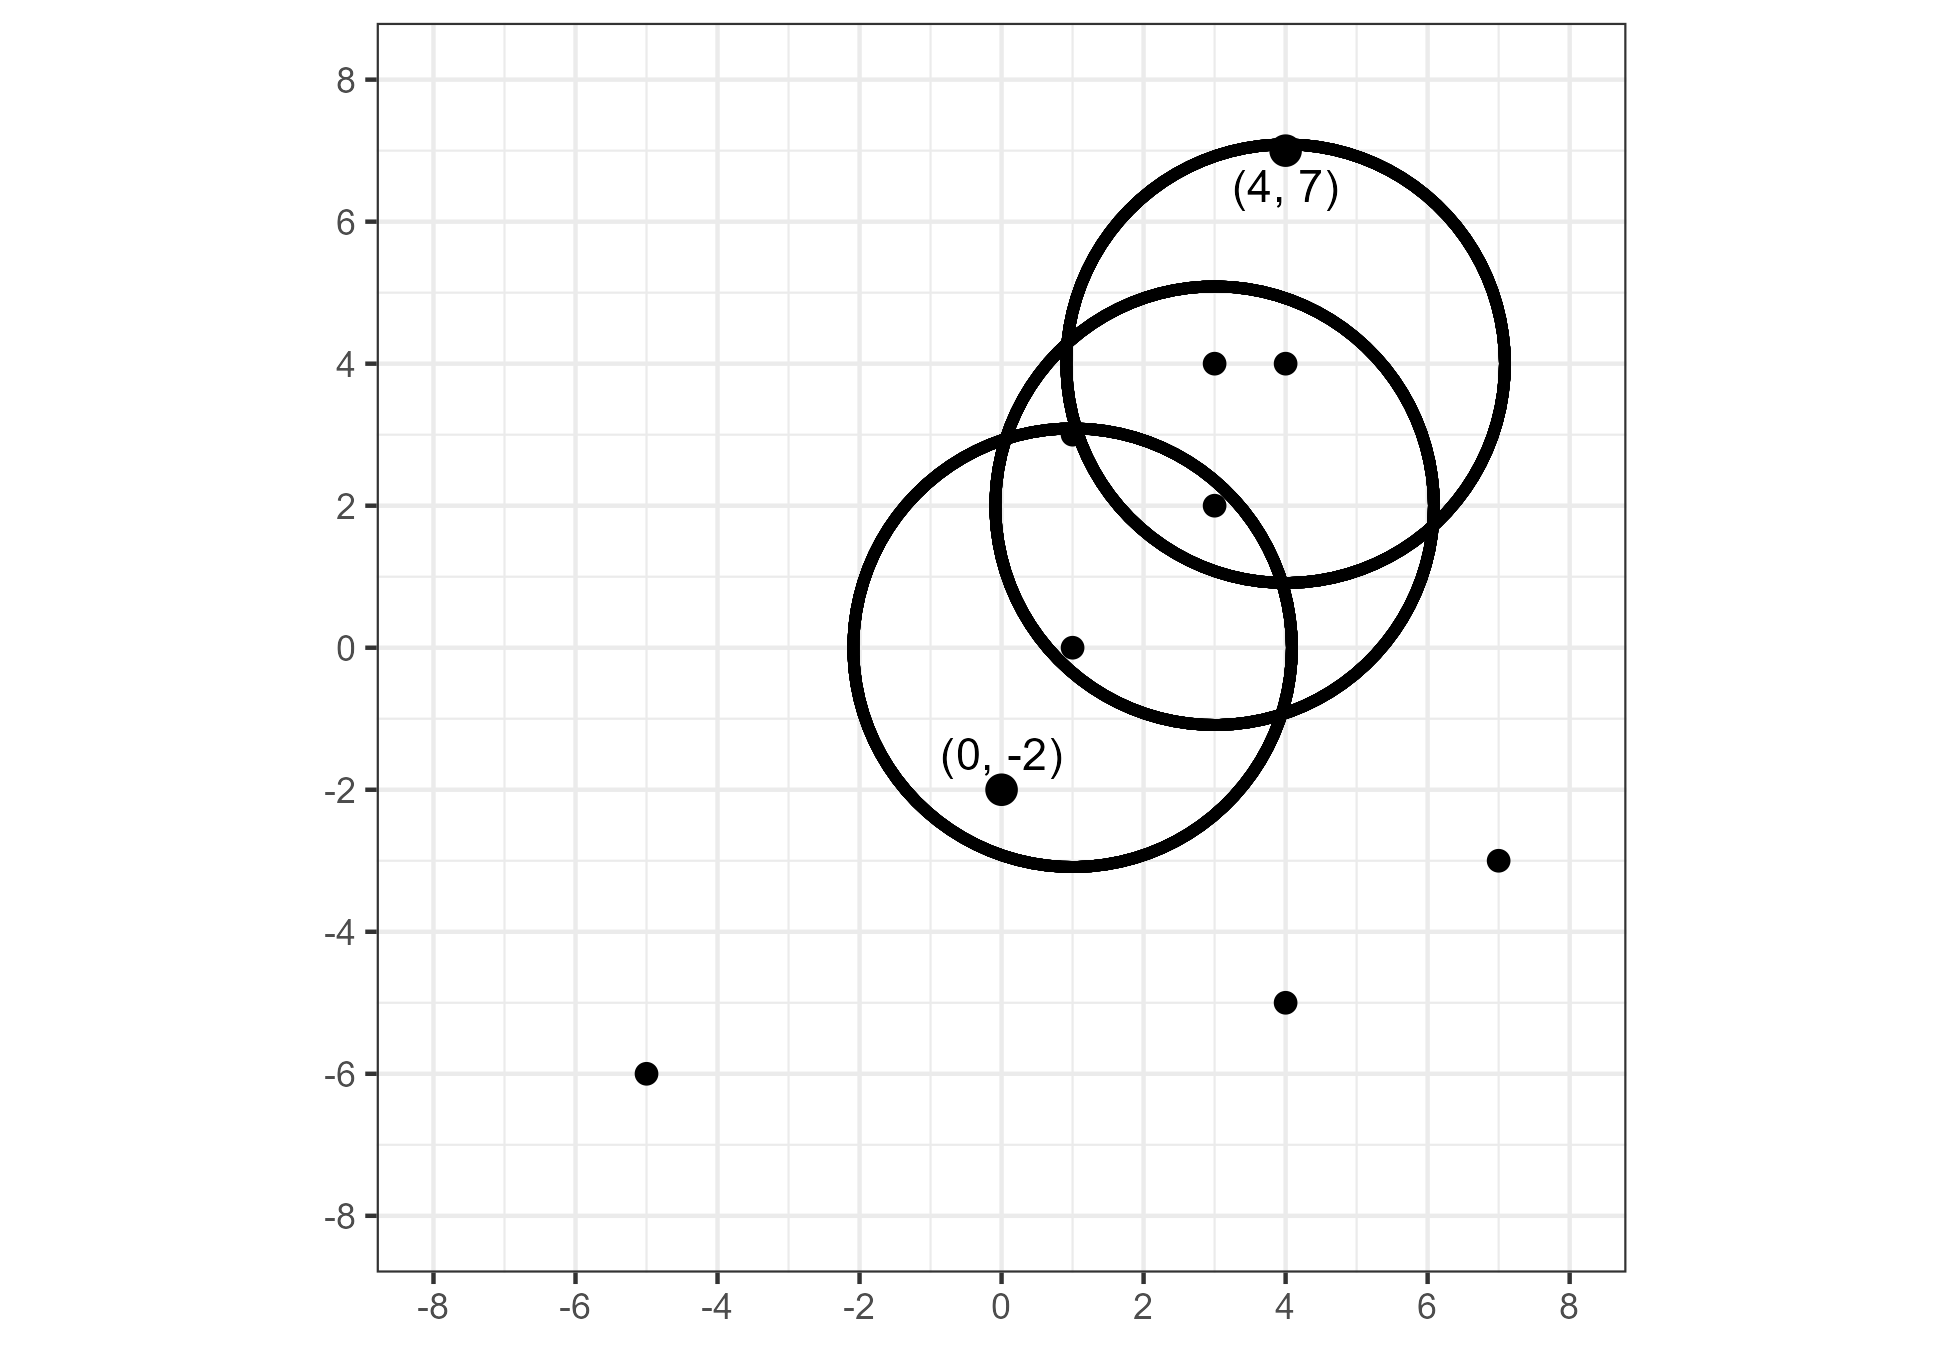
\includegraphics[width=.8\textwidth]{figures/dbscanExample_densityConnected} 

}

\caption{An example of two points that are density-connected, but not density-reachable, with respect to $\epsilon = 3$ and $Minpts = 2$.}\label{fig:densityConnectedExample}
\end{figure}

A \emph{cluster} \(C \subset D\) with respect to \(\epsilon\) and \(Minpts\) satisfies the following conditions:

\begin{enumerate}
\def\labelenumi{\arabic{enumi}.}
\item
  \(\forall x,y\): if \(x \in C\) and \(y\) is density-reachable from \(x\) with respect to \(\epsilon\) and \(Minpts\), then \(y \in C\).
\item
  \(\forall x,y \in C\): \(x\) is density-connected to \(y\) with respect to \(\epsilon\) and \(Minpts\).
\end{enumerate}

For a data set \(D\), the DBSCAN algorithm determines clusters based on the above definition.
Points not assigned to a cluster are classified as \emph{noise points}.
The algorithm halts once all points are assigned to a cluster or classified as noise.

Figure \ref{fig:dbscanResultExample} shows the labels return by DBSCAN for the example considered above with respect to \(\epsilon = 3\) and \(Minpts = 2\).
The algorithm finds a cluster of seven points, colored blue, and classifies three points as noise, colored red.

\begin{figure}[!htbp]

{\centering 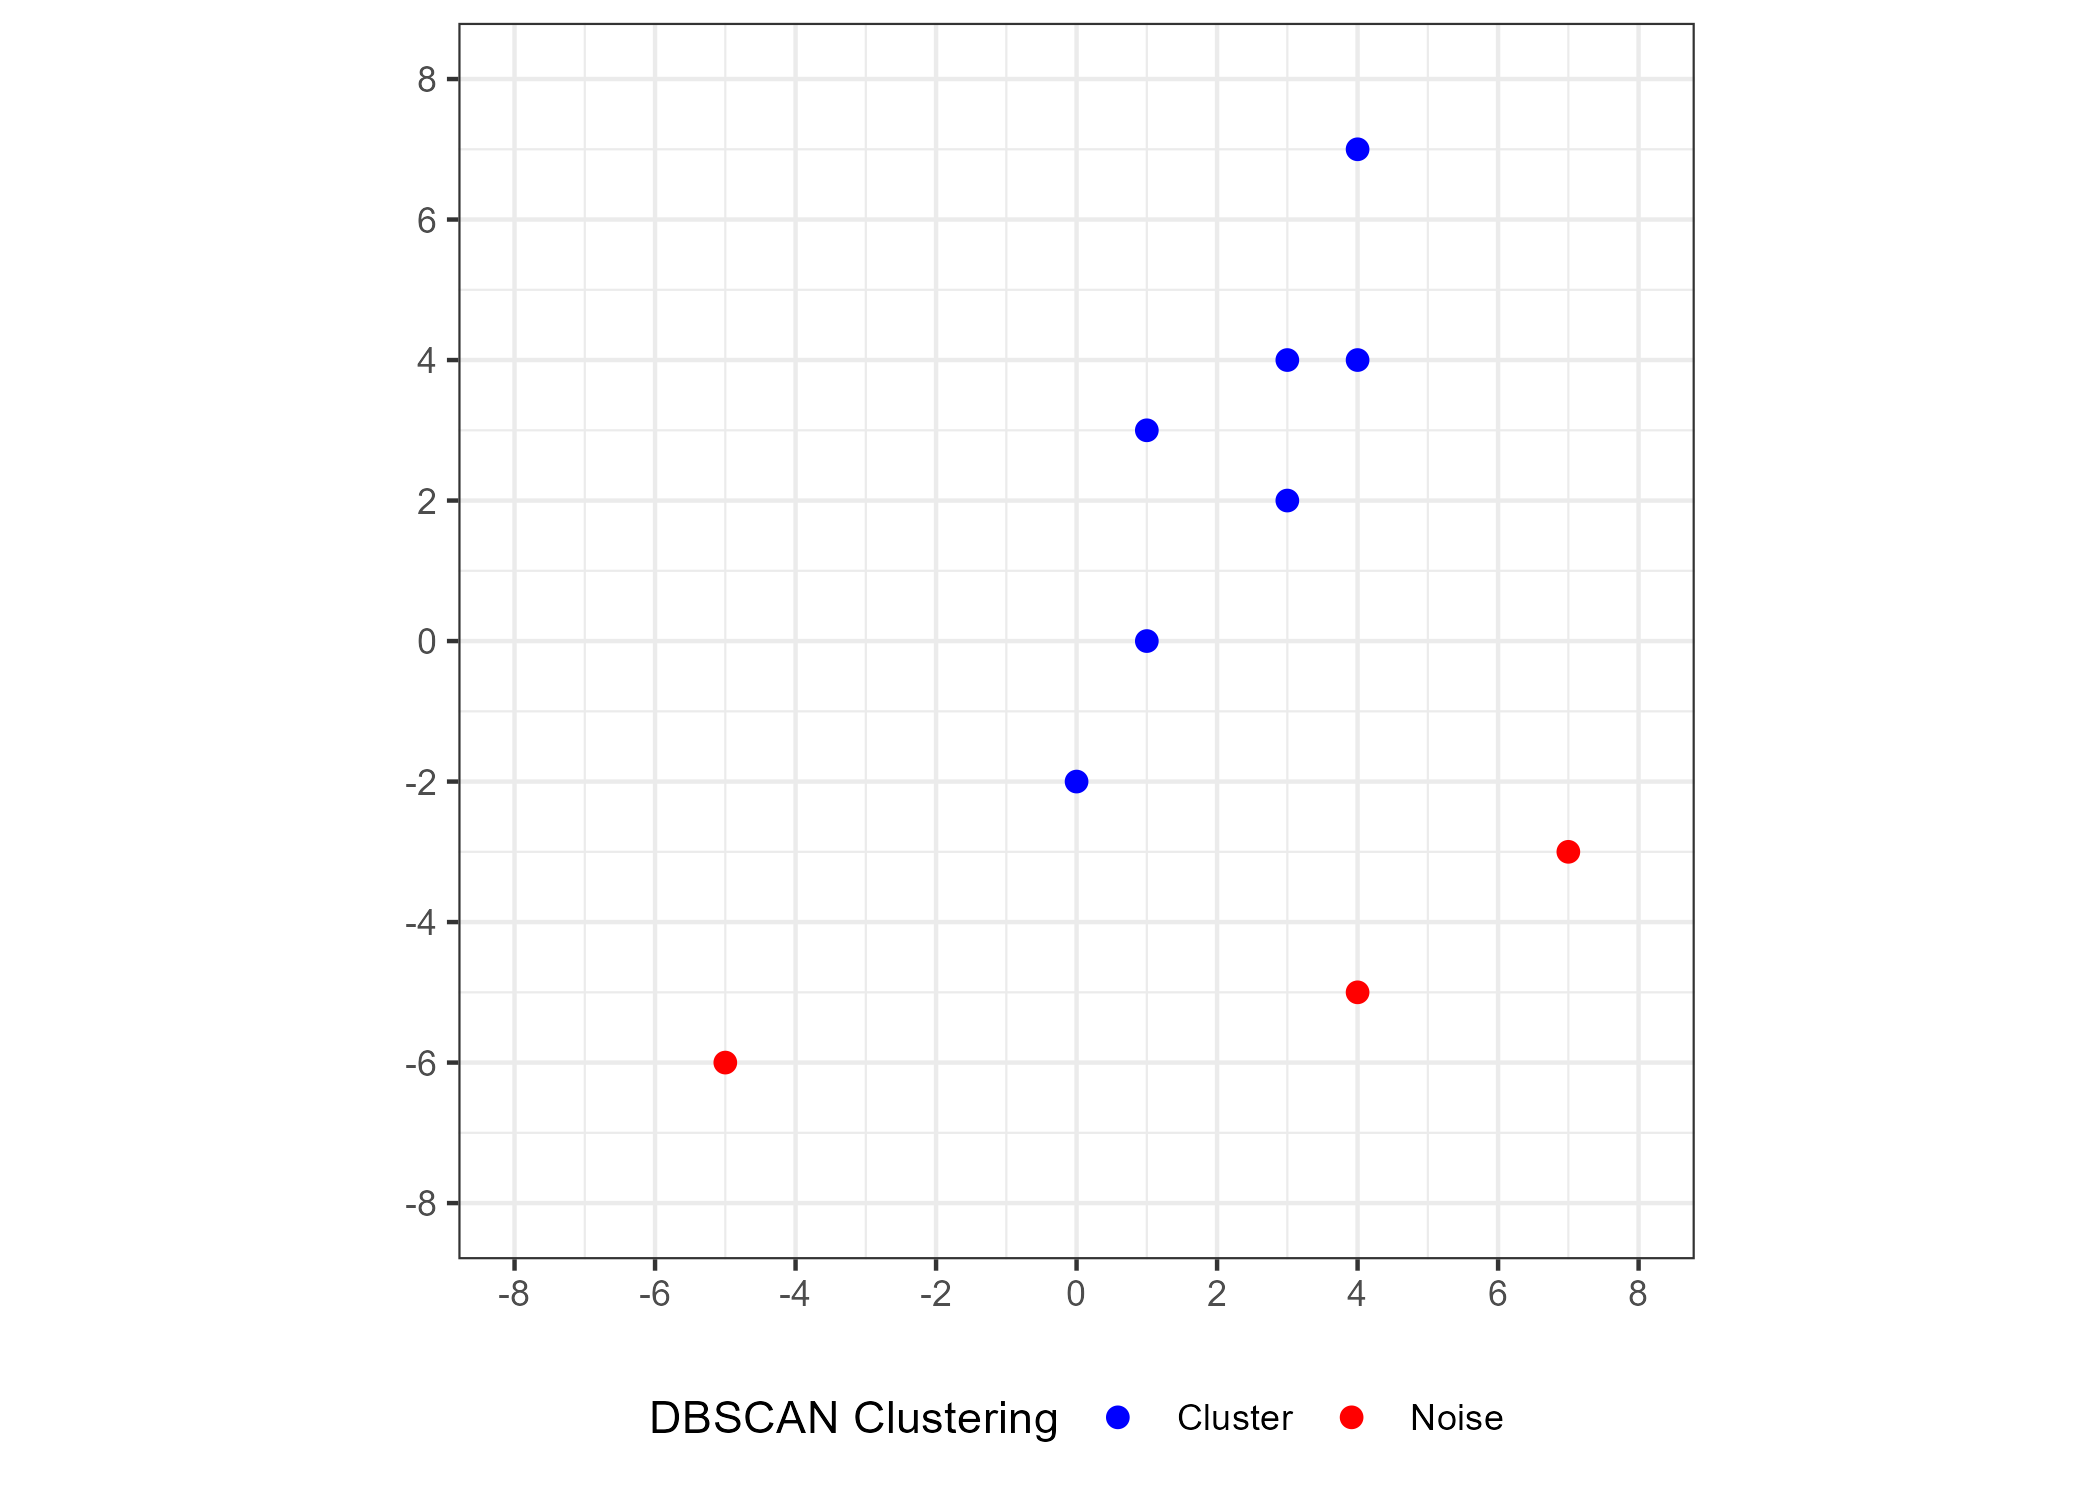
\includegraphics[width=.8\textwidth]{figures/dbscanExample_clusters} 

}

\caption{Cluster labeling for 10 data points using the DBSCAN algorithm with parameters $\epsilon = 3$ and $Minpts = 2$. Seven points are assigned to a single cluster and the remaining three are classified as noise.}\label{fig:dbscanResultExample}
\end{figure}

\hypertarget{implementation-considerations}{%
\subsection{Implementation Considerations}\label{implementation-considerations}}

In the computational sciences, it is one thing to publish code along with research findings.
Publicly-available code and data make results accessible in terms of acquisition.
It is much more challenging to make code \emph{conceptually} accessible to others.
The former allows others to obtain the same results under the same programming conditions while the latter empowers others to actually engage with and potentially improve upon individual pieces of the algorithm.
In any data analysis pipeline, the procedural details may be obscured as the goals of the analysis become more sophisticated.
It is therefore worthwhile to design tools that make the data analysis process both easier to implement and understand \citep{tidy-data}.

Our implementation of the cartridge case comparison pipeline adheres to the ``tidy'' principles of design \citep{tidyverse}.
The ``tidyverse'' is a collection of R packages that share an underlying design philosophy and structure.
Knowledge and skills learned while using one tidy package can be applied to others.
The four principles of a tidy API are:

\begin{enumerate}
\def\labelenumi{\arabic{enumi}.}
\tightlist
\item
  \emph{Reuse existing data structures.}
\end{enumerate}

\begin{quote}
For example, users do not need to learn new data attributes or compatible functions if a package reuses existing data structures.
\end{quote}

\begin{enumerate}
\def\labelenumi{\arabic{enumi}.}
\setcounter{enumi}{1}
\tightlist
\item
  \emph{Compose simple functions with the pipe.}
\end{enumerate}

\begin{quote}
The pipe operator allows the output of one function to be passed as input to another without assigning a new variable. We incrementally transform data as they move from one function to another rather than drastically transforming the data in a single call.
\end{quote}

\begin{enumerate}
\def\labelenumi{\arabic{enumi}.}
\setcounter{enumi}{2}
\tightlist
\item
  \emph{Embrace functional programming.}
\end{enumerate}

\begin{quote}
The functional programming paradigm encourages immutability of objects, meaning data passed as input to a function are not changed.
Rather, the function makes a copy of the input data, manipulates the copy, and returns the transformed copy as output.
This differs from an ``object-oriented'' paradigm where functions have the ability to implicitly rewrite or change the state of the original data.
It is easier to reason about a function that actually returns an object as output than one that changes the input object as a ``side effect.''
\end{quote}

\begin{enumerate}
\def\labelenumi{\arabic{enumi}.}
\setcounter{enumi}{3}
\tightlist
\item
  \emph{Design for humans.}
\end{enumerate}

\begin{quote}
Designing a package for humans largely comes down to using consistent, explicit, and descriptive naming schemes for objects and functions.
\end{quote}

Conceptualizing the cartridge case comparison procedure as a pipeline makes it easier to understand.
We go one step further by actually implementing the procedure as a sequence of algorithms that are programatically connected together in the R statistical programming language \citep{r}.
In particular, we utilize the pipe operator \texttt{\%\textgreater{}\%} available from the magrittr R package \citep{magrittr}.
The pipe operator allows the user to think intuitively in terms of verbs applied to the data.
Table \ref{tab:pipelineTable} illustrates two pipelines that utilize the pipe operator.
The left-hand example shows how an R data frame is manipulated by piping it between functions from the dplyr package.
Functions like \texttt{group\_by}, \texttt{summarize}, and \texttt{filter} are simple building blocks strung together to create complicated workflows.
The right-hand example similarly illustrates a cartridge case object passing through a comparison pipeline.
While the full comparison procedure is complex, the modularization to the \texttt{preProcess\_}, \texttt{comparison\_}, and \texttt{decision\_} steps, which can further be broken-down into simpler functions, renders the process more understandable and flexible for the user.

\begin{table}[!htbp]
\centering
\begin{tabular}{l|l}
Data Frame Manipulation Example & Cartridge Case Comparison Example\\
\hline
\texttt{dataFrame \%>\%} & \texttt{cartridgeCase1 \%>\%} \\
\ \ \texttt{group\_by(category) \%>\%} & \ \ \texttt{preProcess\_func(params1) \%>\%}\\
\ \ \texttt{summarize(x = summary(var)) \%>\%} &\ \ \texttt{comparison\_func(cartridgeCase2,} \\
\ \ \texttt{filter(x > 0) ...} & \hspace{21ex}\texttt{params2) \%>\%} \\
& \ \ \texttt{decision\_func(params3) ...} \\
\end{tabular}
\caption{Two examples of data analysis workflows that utilize the pipe operator. The left side shows a data frame manipulation while the right side shows a comparison of two cartridge cases.}
\label{tab:pipelineTable}
\end{table}

Adherence to tidy principles makes it easier to engage with and understand the overall data analysis pipeline.
In our application it also enables experimentation by making it easy to change one step of the pipeline and measure the downstream effects \citep{reproducibleScience}.
Each step of the cartridge case comparison pipeline requires the user to define parameters.
These can range from minor to substantial, such as choosing the standard deviation used in a Gaussian filter to choosing the algorithm used to calculate a similarity score.
So far, no consensus exists for the ``best'' parameter settings.
A large amount of experimentation is yet required to establish these parameters.
A tidy implementation of the cartridge case comparison pipeline allows more people to engage in the validation and improvement of the procedure.

Figure \ref{fig:taiEddyPreprocess}, Figure \ref{fig:ricePreprocess}, Figure \ref{fig:handwriterPreprocess}, and Figure \ref{fig:cmcRPreprocess} illustrate how various forensic comparison algorithms use a modularized structure to conceptualize their pre-processing procedures.
In each figure, a sequence of modular procedures are applied to a piece of evidence.
Figure \ref{fig:taiEddyPreprocess} shows morphological and image processing procedures applied to a 2D image of a cartridge case to remove the firing pin region \citep{tai_fully_2018}.

\begin{figure}[!htbp]

{\centering 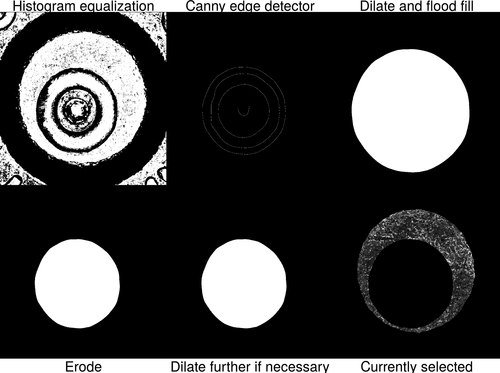
\includegraphics[width=.7\textwidth]{images/taiEddyPreprocess} 

}

\caption{A pre-processing procedure applied to a 2D image of a cartridge case to identify the firing pin impression. The procedure results in a 2D image of a cartridge case without the firing pin impression region.}\label{fig:taiEddyPreprocess}
\end{figure}

Figure \ref{fig:ricePreprocess} shows the procedure by which a 2D ``signature'' of a bullet scan is extracted from a 3D topographical scan \citep{Rice2020}.

\begin{figure}[!htbp]

{\centering 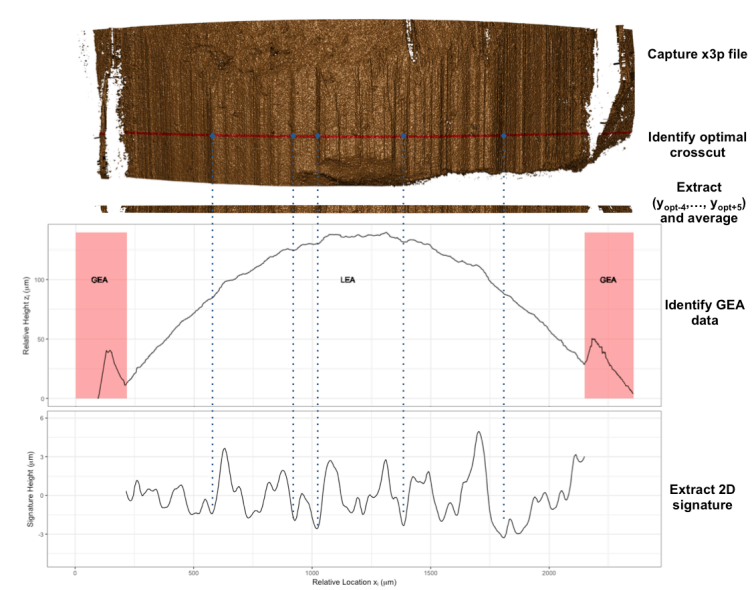
\includegraphics[width=.8\textwidth]{images/riceBulletPreprocessDiagram} 

}

\caption{A pre-processing procedure for extracting 2D bullet \`\`signatures" from a 3D topographic bullet scan. The procedure results in an ordered sequence of values representing the local variations in the surface of the bullet.}\label{fig:ricePreprocess}
\end{figure}

Figure \ref{fig:handwriterPreprocess} shows how an image of the written word ``csafe'' is processed using the handwriter R package to break the word into individual \emph{graphemes} that can be further processed \citep{handwriter}.

\begin{figure}[!htbp]

{\centering 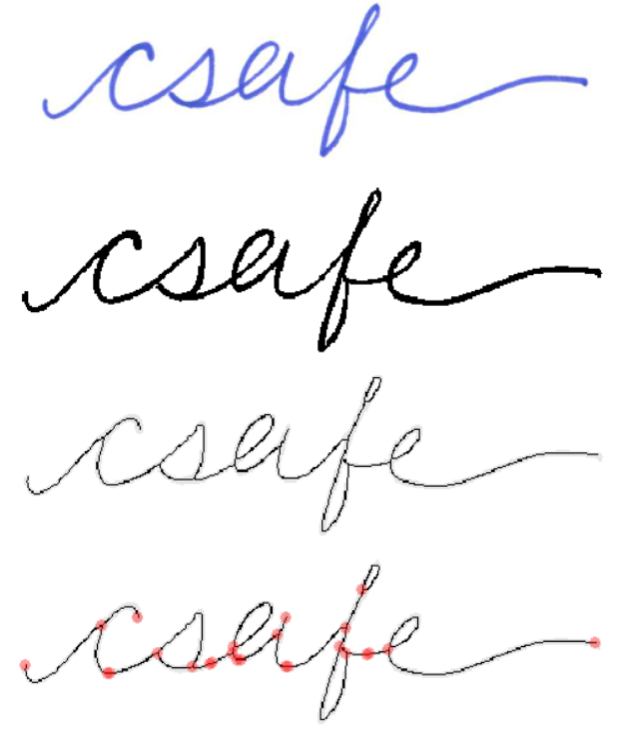
\includegraphics[width=.35\textwidth]{images/handwriterPreprocessDiagram} 

}

\caption{A pre-processing procedure applied to an image of the handwritten word "csafe." The procedure results in a skeletonized version of the word that has been separated into graphemes as represented by orange nodes.}\label{fig:handwriterPreprocess}
\end{figure}

Finally, Figure \ref{fig:cmcRPreprocess} shows a 3D topographical cartridge case scan undergoing various procedures to isolate and highlight the breech face impressions.
These procedures are discussed in greater detail in Chapter 2.

\begin{figure}[!htbp]

{\centering 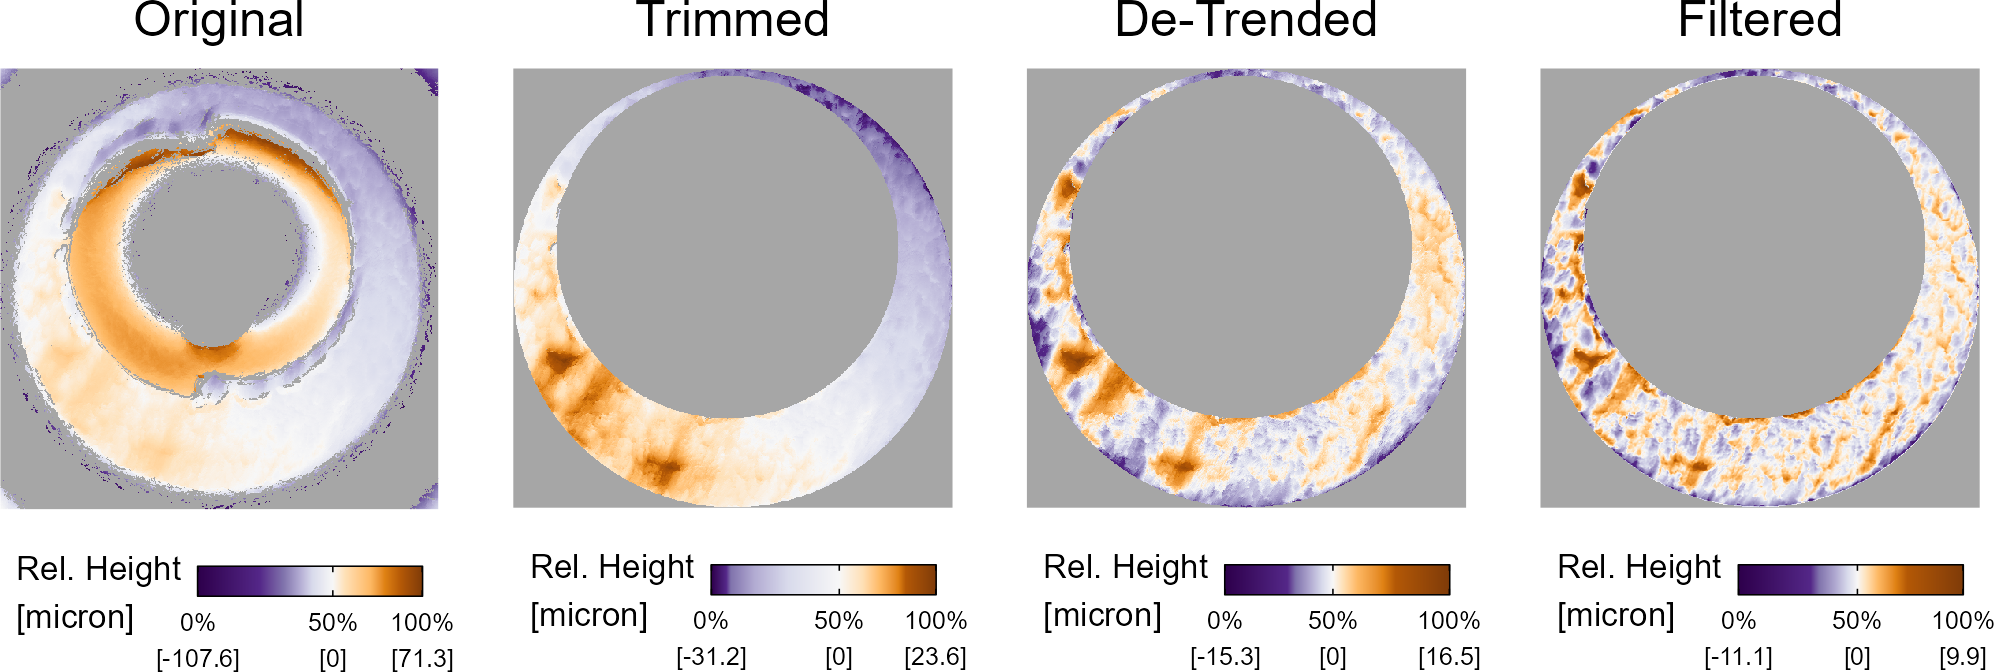
\includegraphics[width=\textwidth]{figures/preProcessPlots} 

}

\caption{A cartridge case undergoing various pre-processing steps. The procedure results in a cartridge case scan in which the breech face impressions have been segmented and highlighted.}\label{fig:cmcRPreprocess}
\end{figure}

By breaking the broader pre-processing step into modularized pieces, we can devise other arrangements of these pre-processing procedures that may improve the segmenting or emphasizing of the region of interest.
The modularity of the pipeline makes it easier to understand what the algorithm is doing ``under the hood.''
A genuine modular implementation enables others to experiment with alternative versions of the pipeline, thus accelerating discovery and improvement.

\hypertarget{a-study-in-reproducibility-the-congruent-matching-cells-algorithm-and-cmcr-package}{%
\chapter{A Study in Reproducibility: The Congruent Matching Cells Algorithm and cmcR package}\label{a-study-in-reproducibility-the-congruent-matching-cells-algorithm-and-cmcr-package}}

\hypertarget{abstract}{%
\section*{Abstract}\label{abstract}}
\addcontentsline{toc}{section}{Abstract}

Scientific research is driven by our ability to use methods, procedures, and materials from previous studies and further research by adding to it.
As the need for computationally-intensive methods to analyze large amounts of data grows, the criteria needed to achieve reproducibility, specifically computational reproducibility, have become more sophisticated.
In general, prosaic descriptions of algorithms are not detailed or precise enough to ensure complete reproducibility of a method.
Results may be sensitive to conditions not commonly specified in written-word descriptions such as implicit parameter settings or the programming language used.
To achieve true computational reproducibility, it is necessary to provide all intermediate data and code used to produce published results.
In this paper, we consider a class of algorithms developed to perform firearm evidence identification on cartridge case evidence known as the \emph{Congruent Matching Cells} (CMC) methods.
To date, these algorithms have been published as textual descriptions only.
We introduce the first open-source implementation of the Congruent Matching Cells methods in the R package cmcR.
We have structured the cmcR package as a set of sequential, modularized functions intended to ease the process of parameter experimentation.
We use cmcR and a novel variance ratio statistic to explore the CMC methodology and demonstrate how to fill in the gaps when provided with computationally ambiguous descriptions of algorithms.

\hypertarget{intro}{%
\section{Introduction}\label{intro}}

Forensic examinations are intended to provide an objective assessment of the probative value of a piece of evidence.
Typically, this assessment of probative value is performed by a forensic examiner who visually inspects the evidence to determine whether it matches evidence found on a suspect.
The process by which an examiner arrives at their evidentiary conclusion is largely opaque and has been criticized \citep{pcast2016} because its subjectivity does not allow for an estimation of error rates.
In response, \citet{council_strengthening_2009} pushed to augment subjective decisions made by forensic examiners with automatic algorithms that objectively assess evidence and can be explained during court testimony.
In addition to the objectivity of these algorithms, there is an additional benefit: we expect that an algorithm with the same random seed run on the same data multiple times will produce the same answer; that is, that the results are repeatable.
This is extremely beneficial because it allows the prosecution and defense to come to the same conclusion given objective evidence or data.

\hypertarget{repeatability-and-reproducibility}{%
\subsection{Repeatability and reproducibility}\label{repeatability-and-reproducibility}}

Repeatability in forensic labs is enforced primarily using standard operating procedures (SOPs), which specify the steps taken for any given evaluation, along with the concentrations of any chemicals used, the range of acceptable machine settings, and any calibration procedures required to be completed before the evidence is evaluated.
When labs use computational procedures, this SOP is augmented with specific algorithms, which are themselves SOPs intended for use by man and machine.
Algorithms are generally described on two levels: we need both the conceptual description (intended for the human using the algorithm) and the procedural definition (which provides the computer hardware with a precise set of instructions).
For scientific and forensic repeatability and reproducibility, it is essential to have both pieces: the algorithm description is critical for establishing human understanding and justifying the method's use in court, but no less important is the computer code which provides the higher degree of precision necessary to ensure the results obtained are similar no matter who evaluates the evidence.
As with SOPs in lab settings, the code parameters function like specific chemical concentrations; without those details, the SOP would be incomplete and the results produced would be too variable to be accepted in court.

The \citet{nasem_2019} defines \emph{reproducibility} as ``obtaining consistent computational results using the same input data, computational steps, methods, code, and conditions of analysis.'' This form of reproducibility requires that the input data, code, method, and computational environment are all described and made available to the community.
In many situations, this level of reproducibility is not provided -- not just in forensics but in many other applied disciplines.
In forensics in particular, it is easier to list the exceptions: reproducible algorithms have been proposed in sub-disciplines including DNA \citep{Tvedebrink2020, osiris, openForSciR}, glass \citep{Curran2000, Park2019}, handwriting \citep{crawford_handwriting_2020}, shoe prints \citep{park_algorithm_2020}, and ballistic evidence \citep{hare_automatic_2016, tai_fully_2018}.

We find it useful to instead consider a more inclusive hierarchy of reproducibility.
Algorithms at higher tiers of the hierarchy are more easily reproducible in the sense that fewer resources are required to (re)-implement the algorithm.

\textbf{Definition 1} \emph{Hierarchy of Reproducibility}

\begin{quote}
\textbf{Conceptual description} \emph{The algorithm is described and demonstrated in a scientific publication.}
\end{quote}

\begin{quote}
\textbf{Pseudocode} \emph{The algorithm is described at a high level of detail with pseudocode implementation provided, and results are demonstrated in a scientific publication.}
\end{quote}

\begin{quote}
\textbf{Reproducible data} \emph{The algorithm is described and demonstrated in a scientific publication, and input data are available in supplementary material.}
\end{quote}

\begin{quote}
\textbf{Comparable results} \emph{The algorithm is described and demonstrated in a scientific publication, and input data and numerical results are provided in supplementary material.}
\end{quote}

\begin{quote}
\textbf{Full reproducibility} \emph{The algorithm is described and demonstrated in a scientific publication, and the input data, source code, parameter settings, and numerical results are provided in supplementary material.}
\end{quote}

To aid in comprehension of an algorithm, it is useful to supplement conceptual descriptions with pseudocode.
However, a conceptual description and pseudocode alone do not contain sufficient detail (e.g., parameter settings) to ensure computational reproducibility.
Implementing algorithms based on conceptual descriptions or pseudocode requires enumerating and testing possible parameter choices which, depending on their complexity, can be a lengthy and expensive process.
In contrast, implementing fully reproducible algorithms requires only as much time as it takes to emulate the original development environment.
Commonly identified reasons for unreproducible results include (1) ambiguity in how procedures were implemented, (2) missing or incomplete data, and (3) missing or incomplete computer code to replicate all statistical analyses \citep{leek_is_2017}.
In particular, for statistical algorithms which depend on input data, we find that full reproducibility depends on the provision of both original data and any manual pre-processing applied to said data, as this manual process is not reproducible by itself.
In combination with the code, the algorithm description, and the numerical results presented in the paper, it should be possible to fully reproduce the results of a paper.

In this paper, we demonstrate the importance of higher levels of reproducibility by examining the Congruent Matching Cells (CMC) algorithm for cartridge case comparisons and developing an open-source, fully reproducible version for general use in the forensics community.

\hypertarget{the-congruent-matching-cells-algorithm}{%
\subsection{The Congruent Matching Cells algorithm}\label{the-congruent-matching-cells-algorithm}}

A \emph{cartridge case} is the portion of firearm ammunition that encases a projectile (e.g., bullet, shots, or slug) along with the explosive used to propel the projectile through the firearm.
When a firearm is discharged, the projectile is propelled down the barrel of the firearm, while the cartridge case is forced towards the back of the barrel.
It strikes the back wall, known as the \emph{breech face}, of the barrel with considerable force, thereby imprinting any markings on the breech face onto the cartridge case and creating the so-called \emph{breech face impressions}.
These markings are used in forensic examinations to determine whether two cartridge cases have been fired by the same firearm.
During a forensic examination, two pieces of ballistic evidence are placed under a \emph{comparison microscope}.
Comparison microscopes allow for a side-by-side comparison of two objects within the same viewfinder, as seen in Figure \ref{fig:ccPair}.
A pair of breech face images is aligned along the thin black line in the middle of the images.
The degree to which these breech face markings can be aligned is used to determine whether the two cartridge cases came from the same source; i.e., were fired from the same firearm.
These breech face impressions are considered analogous to a firearm's ``fingerprint'' left on a cartridge case \citep{Thompson2017}.

\begin{figure}[htbp]

{\centering 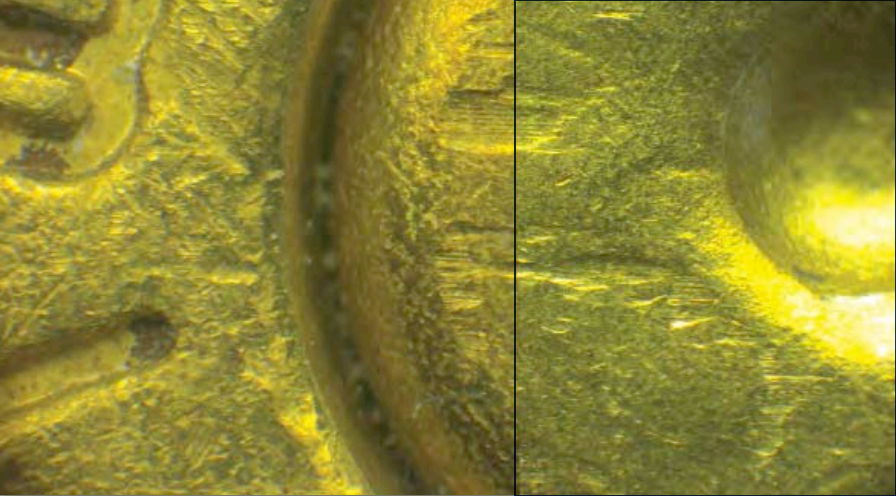
\includegraphics[width=12.44in]{images/cartridgeCasePair_comparison_with_line} 

}

\caption{A cartridge case pair with visible breech face impressions under a microscope.  A thin line can be seen separating the two views. The degree to which the markings coincide is used to conclude whether the pair comes from the same source.}\label{fig:ccPair}
\end{figure}

The Congruent Matching Cells (CMC) pipeline is a collection of algorithms to process and compare cartridge case evidence \citep{song_proposed_2013}.
Since its introduction, the pipeline and its extensions \citep{tong_improved_2015, chen_convergence_2017, song_estimating_2018} have shown promise in being able to differentiate between matching and non-matching cartridge cases.
However, so far the CMC pipelines have only been introduced in the form of conceptual descriptions.
Further, the cartridge case scans used to validate the pipelines are only available in their raw, unprocessed forms on the NIST Ballistics Toolmark Research Database \citep{nbtrd}.
While it is clear that the creators of the CMC pipeline have a working implementation, the wider forensic science community only has access to conceptual descriptions of the pipeline and summary statistics describing its performance.
In our hierarchy of reproducibility, this puts the CMC algorithm somewhere between the conceptual description and reproducible data stage: the steps are described but no code is available, and the raw data are available but manual pre-processing steps make this raw data insufficient to replicate the pipeline even with newly written code.

The development of the CMC algorithm seems to be representative of how many forensic algorithms are developed: after an algorithm is introduced, researchers build upon the foundation laid by the original algorithm in subsequent papers.
These changes are often incremental in nature and reflect a growing understanding of the algorithm's behavior.
While this cycle of scientific progress certainly is not unique to forensic algorithms, given the gravity of the application it is imperative that these incremental improvements not be unnecessarily delayed.
As such, we believe that the forensic community at-large would benefit greatly by establishing an open-source foundation for their algorithms upon which additional improvements can be developed.
Using open-source algorithms are cheaper to use than writing one's own code, enables the process of peer review by providing an accessible benchmark, and helps other research groups or companies stay on the leading edge of technology development \citep{linux}.

Here, we describe the process of implementing the CMC pipeline for the comparison of marks on spent cartridge cases, using the descriptions from two published papers, \citet{song_3d_2014} and \citet{tong_improved_2015}.
Our R package, cmcR, provides an open-source implementation of the CMC pipeline.
We use cmcR to illustrate how ambiguities in the textual description of an algorithm can lead to highly divergent results.
In particular, our implementation highlights an extreme sensitivity to processing and parameter decisions that has not been discussed previously.
Additionally, we argue that our implementation can be used as a template for future implementations of forensic pattern-matching algorithms to not only ensure transparency and auditability, but also to facilitate incremental improvements in forensic algorithms.

In the remainder of this paper, we describe a general, reproducible, and open-source CMC pipeline which encompasses those discussed in \citet{song_proposed_2013}, \citet{song_3d_2014}, and \citet{tong_improved_2015}.
\citet{song_proposed_2013} lays out the conceptual framework for the original CMC pipeline later implemented in \citet{song_3d_2014} and \citet{tong_fired_2014}.
An improvement of the pipeline presented in \citet{tong_improved_2015} and used in subsequent papers is referred to as the ``High CMC'' method \citep{chen_convergence_2017}. However, it should be noted that what the authors refer to as the original and High CMC decision rules are variations of one step of a larger CMC pipeline.

The cmcR package contains implementations designed for use with 3D topographical scans of the original decision rule described in \citet{song_proposed_2013} and \citet{song_3d_2014} and the High CMC decision rule described in \citet{tong_improved_2015}.
The source code to the full cmcR package is accessible at \url{https://github.com/CSAFE-ISU/cmcR}.

\hypertarget{cmcMethod}{%
\section{The CMC pipeline}\label{cmcMethod}}

In this section, we examine the process of implementing the CMC pipeline for automatic comparisons of 3D cartridge case scans.
At each step, we will discuss how we filled in the gaps of the original description during the creation of cmcR.

All of the CMC pipelines can be broken down into three broad stages: (1) pre-processing, (2) cell-based similarity feature extraction, and (3) application of a decision rule as illustrated in @(fig:overview-flow).
In the following sections we break each of these stages further into a set of modular steps.
One advantage of modularizing these algorithms is that we can implement an algorithm as a set of sequential procedures.
This allows us to test new variations against the old implementation in a coherent, unified framework.

\begin{figure}[htbp]

{\centering 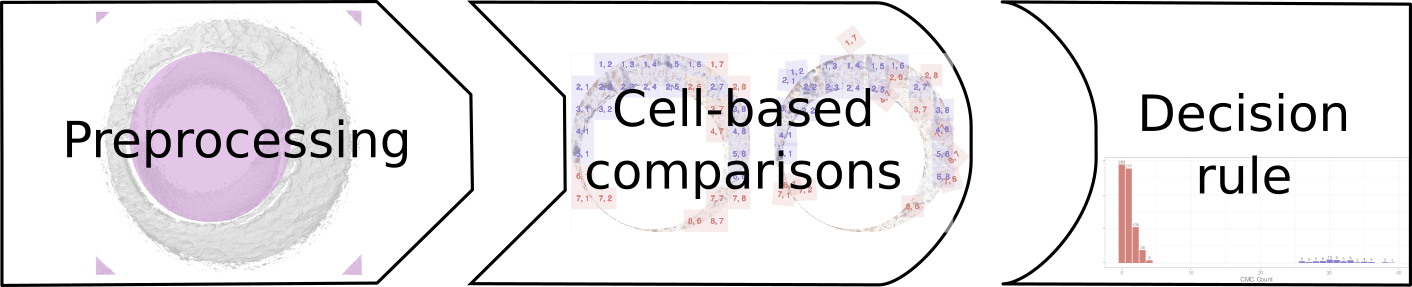
\includegraphics[width=19.61in]{images/overview-flow} 

}

\caption{The stages of CMC pipelines. In the pre-processing stage, each scan is prepared for analysis, removing extraneous information and noise. Then, each scan is broken up into cells, which are numerically compared to cells in the other scan to determine an optimal alignment. Finally, each of the scores arising from the cells in the second stage are compared to a reference distribution to determine whether the scans originate from the same source or from different sources.}\label{fig:overview-flow}
\end{figure}

The primary difference between the two pipelines presented here, using the original and High CMC decision rules, lies in how the decision rules are utilized to separate matching vs.~non-matching cartridge case pairs.
In addition, there are also several small differences in the parameters used in the pre-processing and comparison procedures.

\hypertarget{initialData}{%
\subsection{Initial data}\label{initialData}}

Digital microscopy is capable of precision measurements of surface topology at high resolutions.
Using a 3D microscope, we can obtain scans of breech face impressions at the micron level (\(1 \mu m = 10^{-3} mm = 10^{-6} m\)).
These 3D topological scans are used as input to automated comparison algorithms, such as the CMC pipeline originally proposed in \citet{song_proposed_2013}.
We will use the same data set referenced in \citet{song_3d_2014} and \citet{tong_improved_2015} to illustrate usage of the cmcR package.
These 3D scans of cartridge cases are available from the NIST Ballistics Toolmark Research Database \citep{nbtrd}.
The strings defined below refer to three cartridge case scans available on the NBTRD from \citet{fadul_empirical_2011} and will be used throughout the remainder of this paper.

\begin{Shaded}
\begin{Highlighting}[]
\FunctionTok{library}\NormalTok{(cmcR)}

\NormalTok{nbtrd\_url }\OtherTok{\textless{}{-}} \StringTok{"https://tsapps.nist.gov/NRBTD/Studies/CartridgeMeasurement"}

\NormalTok{x3p\_ids }\OtherTok{\textless{}{-}} \FunctionTok{c}\NormalTok{(}\StringTok{"DownloadMeasurement/2d9cc51f{-}6f66{-}40a0{-}973a{-}a9292dbee36d"}\NormalTok{,}
             \StringTok{"DownloadMeasurement/cb296c98{-}39f5{-}46eb{-}abff{-}320a2f5568e8"}\NormalTok{,}
             \StringTok{"DownloadMeasurement/8ae0b86d{-}210a{-}41fd{-}ad75{-}8212f9522f96"}\NormalTok{)}

\NormalTok{file\_names }\OtherTok{\textless{}{-}} \FunctionTok{c}\NormalTok{(}\StringTok{"fadul1{-}1.x3p"}\NormalTok{,}\StringTok{"fadul1{-}2.x3p"}\NormalTok{,}\StringTok{"fadul2{-}1.x3p"}\NormalTok{)}

\NormalTok{purrr}\SpecialCharTok{::}\FunctionTok{walk2}\NormalTok{(}\AttributeTok{.x =}\NormalTok{ x3p\_ids,}
             \AttributeTok{.y =}\NormalTok{ file\_names,}
             \AttributeTok{.f =} \ControlFlowTok{function}\NormalTok{(x3p\_id,file\_name)\{}
               \FunctionTok{download.file}\NormalTok{(}\AttributeTok{url =} \FunctionTok{file.path}\NormalTok{(nbtrd\_url, x3p\_id),}
                             \AttributeTok{destfile =} \FunctionTok{paste0}\NormalTok{(}\StringTok{"data/"}\NormalTok{,file\_name),}\AttributeTok{mode =} \StringTok{"wb"}\NormalTok{)}
\NormalTok{             \})}
\end{Highlighting}
\end{Shaded}

Cartridge case scans are commonly stored in the ISO standard x3p file format \citep{ISO25178-72}.
x3p is a container format which consists of a single surface matrix representing the height value of the breech face surface and metadata concerning the parameters under which the scan was taken (size, resolution, creator, microscope, microscopy software versions, etc.).
The x3ptools package provides functionality to work with the format in R \citep{x3ptools}.

Figure \ref{fig:cartridgeCasePair-latex} shows the surface matrices of a known match (KM) pair of cartridge cases from a study by \citet{fadul_empirical_2011}.
In this study, a total of 40 cartridge cases were scanned with a lateral resolution of 6.25 microns (micrometers) per pixel.
The surface matrices are approximately \(1200 \times 1200\) pixels in size corresponding to an area of about \(3.8 \times 3.8\) mm\(^2\).

\begin{figure}[htbp]

{\centering \subfloat[\label{fig:cartridgeCasePair-latex-1}]{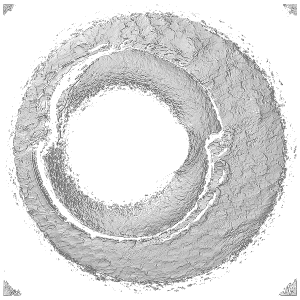
\includegraphics[width=.49\linewidth,height=.49\linewidth]{figures/fadul1-1} }\subfloat[\label{fig:cartridgeCasePair-latex-2}]{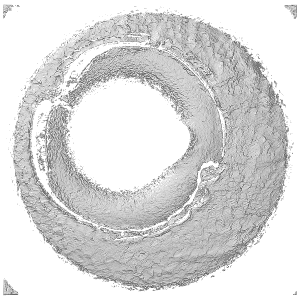
\includegraphics[width=.49\linewidth,height=.49\linewidth]{figures/fadul1-2} }

}

\caption{Unprocessed surface matrices of the known-match Fadul 1-1 and Fadul 1-2 Fadul et al. \(2011\). The observations in the corners of these surface matrices are artifacts of the staging area in which these scans were taken. The holes on the interior of the primer surfaces are caused by the firing pin striking the primer during the firing process. The region of the primer around this hole does not come into uniform contact with the breech face of the firearm.}\label{fig:cartridgeCasePair-latex}
\end{figure}

Only certain regions of a cartridge case contain identifying breech face impression markings.
\citet{song_proposed_2013} defines ``valid correlation regions'' as regions where ``the individual characteristics of the ballistics signature are found that can be used effectively for ballistics identification.''
Prior to applying the CMC comparison procedure, cartridge scans must undergo some pre-processing to isolate the valid correlation regions.

\hypertarget{preProcessing}{%
\subsection{Pre-processing procedures}\label{preProcessing}}

During the pre-processing stage, we apply sequential steps to prepare each cartridge case for analysis.
The goal of this process is to remove the edges and center of the scan which did not come into contact with the breech face, as well as any artifacts of the scan and microscope staging which do not accurately represent the breech face surface.
The various iterations of the CMC algorithm describe different variations of these steps.
A summary of these steps is shown in Figure \ref{fig:pre-processing-schematic}.

\begin{figure}[!htbp]

{\centering 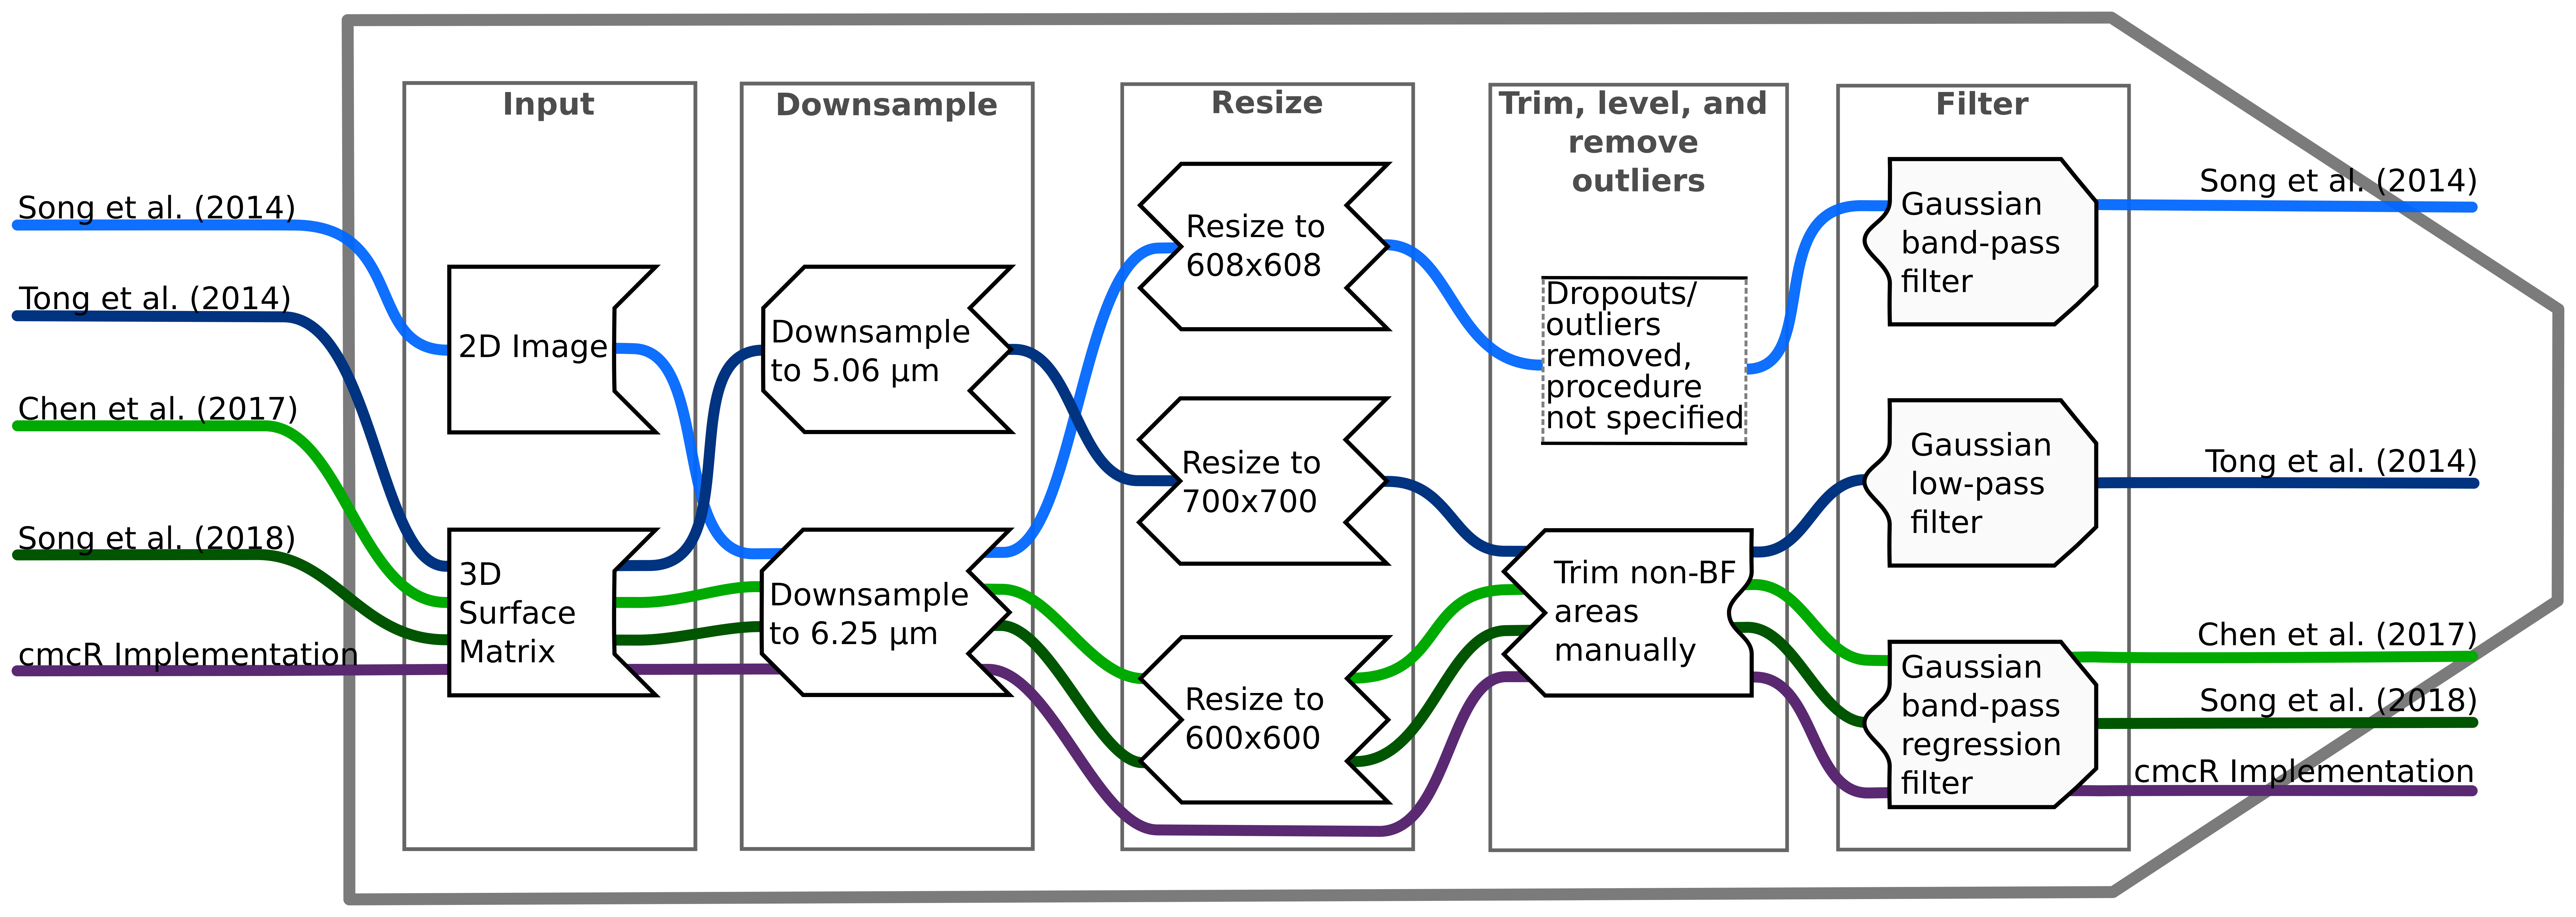
\includegraphics[width=115.54in]{images/preprocessing_flow} 

}

\caption{Overview of the set of pre-processing steps used in the CMC algorithms. Where a procedure step is not discussed or explicitly not applied in the paper, the path traverses empty space.}\label{fig:pre-processing-schematic}
\end{figure}

Translating the pre-processing steps in Figure \ref{fig:pre-processing-schematic} into an implementation requires the implementer to decide between potentially many implicit parameter choices.
For example, Table \ref{tab:pre-processTable} compares the pre-processing procedures as described in \citet{song_3d_2014} to considerations that need to be made when implementing the procedures.
Depending on one's interpretation of the description, there are many possible implementations that satisfy the described procedure - in contrast, there was only one implementation that led to the original results.
While not explicitly mentioned in \citet{song_3d_2014}, \citet{song_estimating_2018} indicates that the ``trimming'' of the unwanted regions of the scan is performed manually.
It is difficult to replicate manual steps as part of a reproducible pipeline; the best solution is for the authors to provide intermediate data after the manual steps have been completed.

\renewcommand{\arraystretch}{2}

\begin{table}

\caption{\label{tab:pre-processTable}Description of pre-processing procedures from Song et al. \(2014\) vs. considerations that need to be made when implementing these procedures. Each of these considerations requires the implementer to decide between potentially many choices.}
\centering
\begin{tabu} to \linewidth {>{\raggedright}X>{\raggedright}X}
\toprule
\textbf{Description from Song et al. (2014)} & \textbf{Implementation Considerations}\\
\midrule
"Trim off the inside firing pin surface and other areas outside the breech face mark, so that only breech face impression data remain for correlation." & Removal of firing pin hole, primer exterior, global trend, and primer roll-off\\
"Identify and remove dropouts or outliers." & Definition of outliers, what "removal" of dropouts or outliers means\\
"Apply a band-pass Gaussian regression filter with 40 $\mu$m short cut-off length and 400 $\mu$m long cut-off length to remove low frequency components, including surface curvature, form error, waviness and high frequency components which mainly arise from the instrument noise." & Wavelength cut-off parameters, specific implementation of the filter\\
\bottomrule
\end{tabu}
\end{table}

The pre-processing procedures are implemented via modularized functions of the form \texttt{preProcess\_*}.
Modularizing the steps of the pre-processing procedures makes the overall process easier to understand and allows for experimentation.
Figure \ref{fig:processingPipeline} shows an overview of the pre-processing framework for the Fadul 1-1 breech face from reading the scan (left) to an analysis-ready region (right).
For each scan in Figure \ref{fig:processingPipeline}, eleven height value percentiles: the Minimum (0th), 1st, 2.5th, 10th, 25th, Median (50th), 75th, 90th, 97.5th, 99th, and Maximum (100th) are mapped to a purple-to-orange color gradient.
This mapping is chosen to highlight the extreme values in each scan.

\begin{figure}[htbp]

{\centering 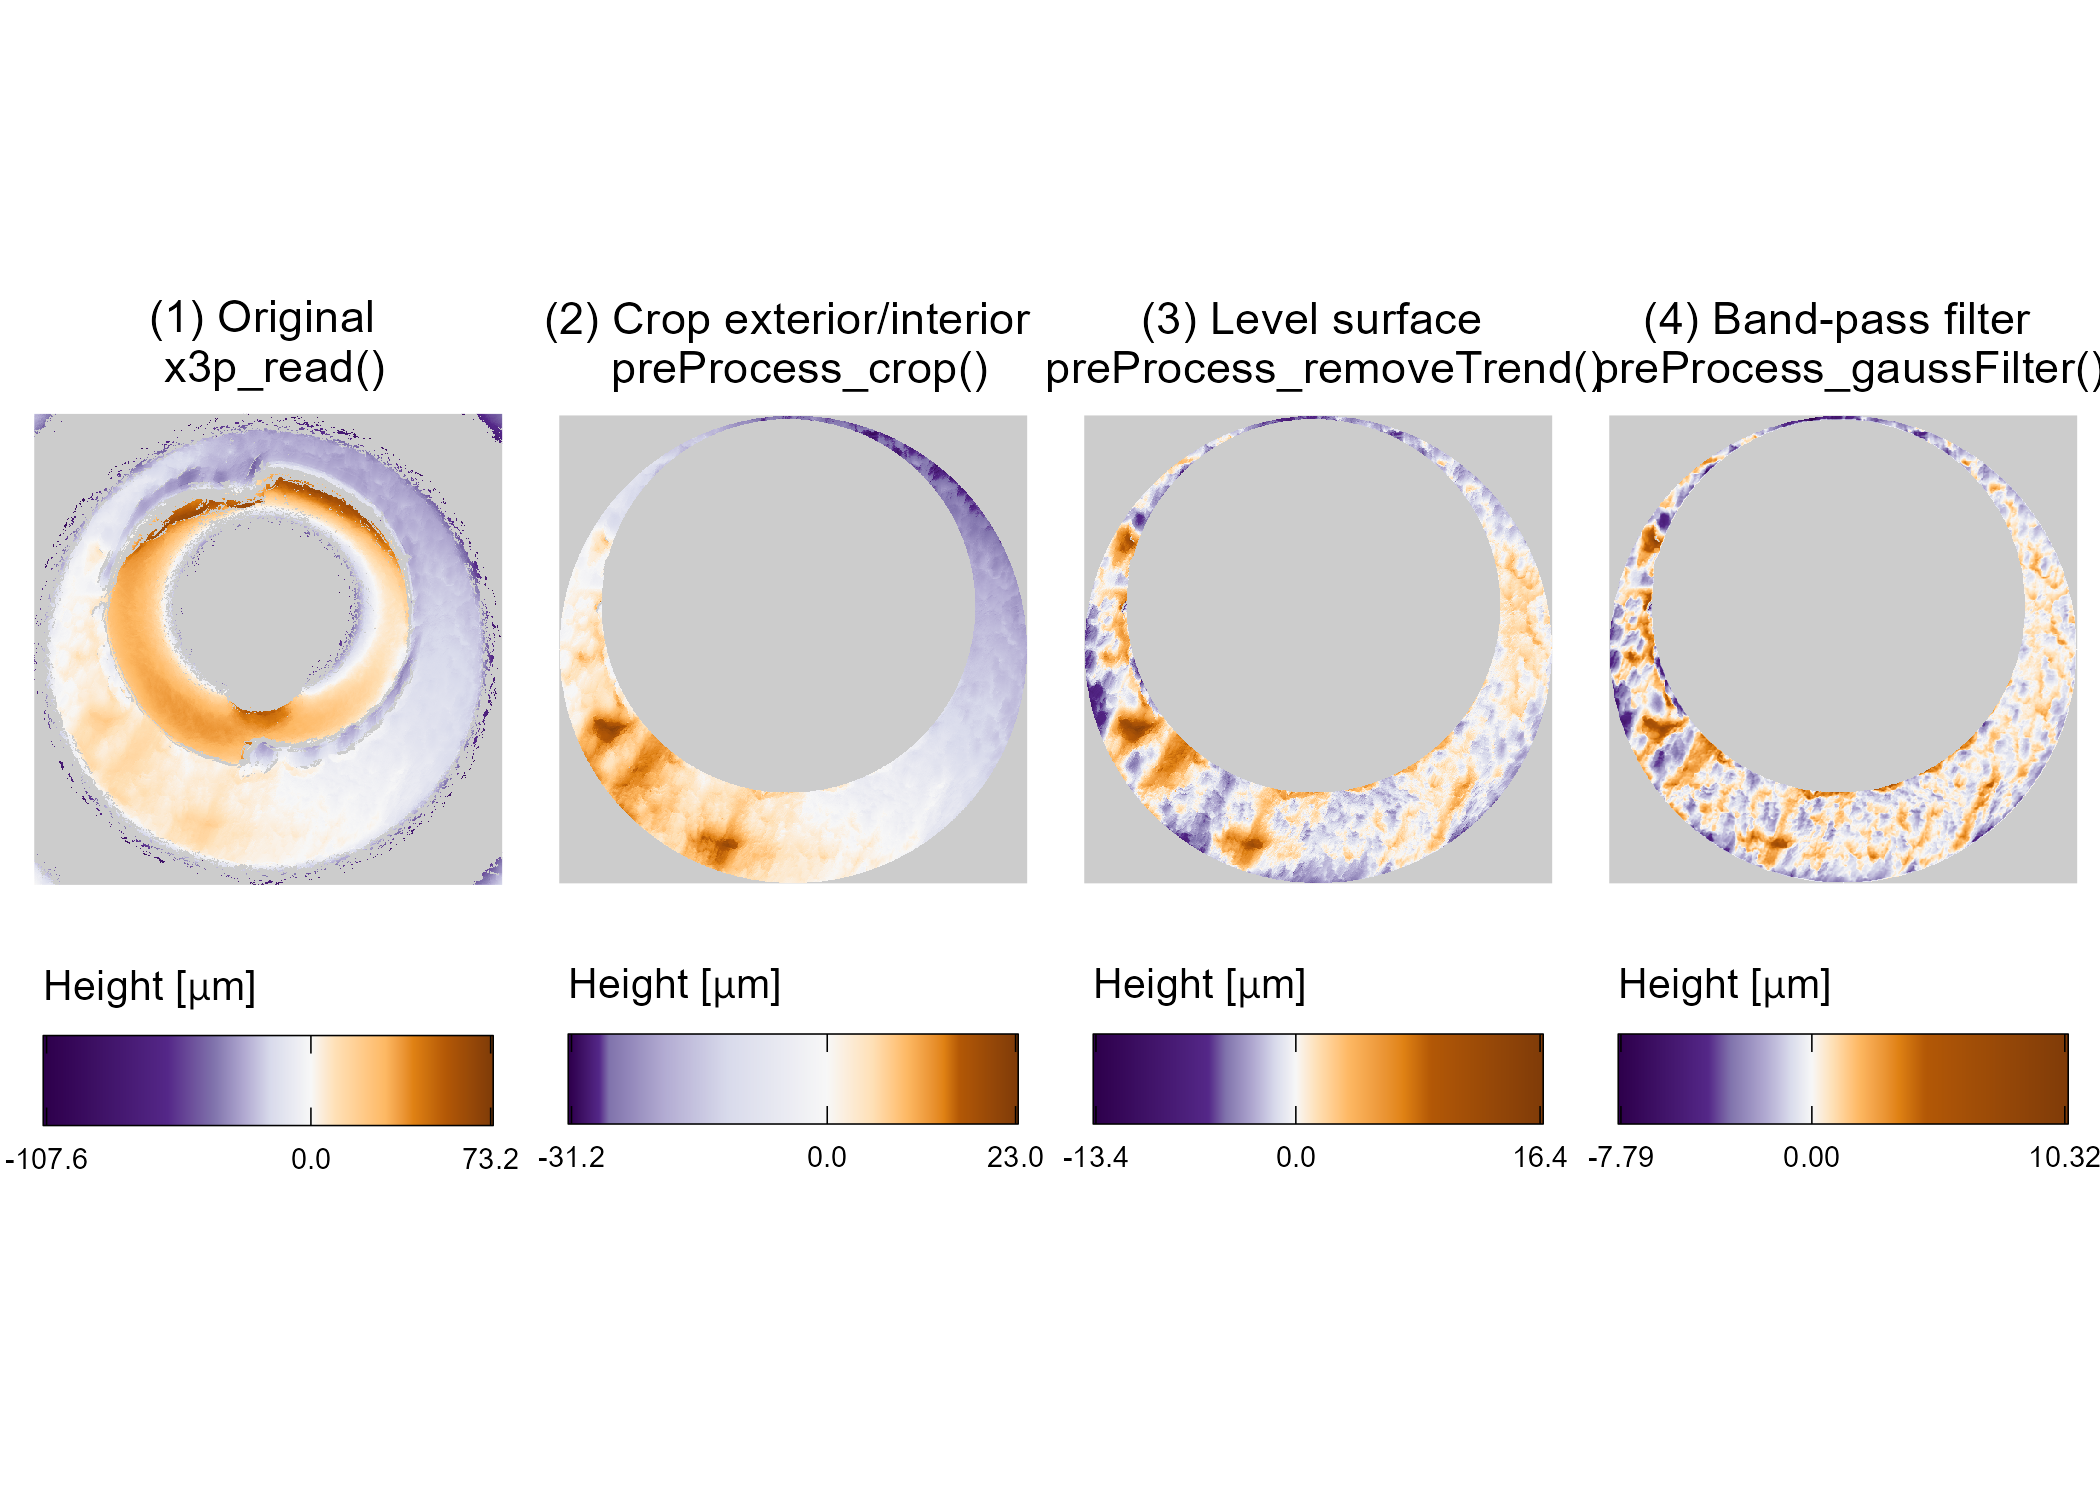
\includegraphics[width=27.08in]{figures/preProcessPipeline} 

}

\caption{Illustration of the sequential application of pre-processing steps implemented in cmcR. We map the cartridge case surface height values to a divergent purple-white-orange color scale to emphasize deviations from the median height value (represented here as 0 micrometers). At each stage, the variability in height across the scan decreases as we emphasize the regions containing breech face impressions.}\label{fig:processingPipeline}
\end{figure}

We demonstrate usage of the \texttt{preProcess\_*} functions on the Fadul 1-1 scan.
Each code chunk is followed up with an explanation of the functions used.

\begin{Shaded}
\begin{Highlighting}[]
\CommentTok{\# Step (1)}
\NormalTok{fadul1}\FloatTok{.1} \OtherTok{\textless{}{-}}\NormalTok{ x3ptools}\SpecialCharTok{::}\FunctionTok{x3p\_read}\NormalTok{(}\StringTok{"data/fadul1{-}1.x3p"}\NormalTok{)}
\end{Highlighting}
\end{Shaded}

We begin with a 3D scan.
Typically, we downsample scans to about 25\% of their size by only retaining every other row and column in the surface matrix.
The breech faces in \citet{fadul_empirical_2011} were initially scanned at a resolution of 3.125 \(\mu\)m per pixel.
Downsampling reduces the resolution to 6.25 \(\mu\)m per pixel.
Step (1) in Figure \ref{fig:processingPipeline} shows an unprocessed breech face scan.

\begin{Shaded}
\begin{Highlighting}[]
\CommentTok{\# Step (2)}
\NormalTok{fadul1}\FloatTok{.1}\NormalTok{\_cropped }\OtherTok{\textless{}{-}}\NormalTok{ fadul1}\FloatTok{.1} \SpecialCharTok{\%\textgreater{}\%}
\NormalTok{  cmcR}\SpecialCharTok{::}\FunctionTok{preProcess\_crop}\NormalTok{(}\AttributeTok{region =} \StringTok{"exterior"}\NormalTok{) }\SpecialCharTok{\%\textgreater{}\%}
\NormalTok{  cmcR}\SpecialCharTok{::}\FunctionTok{preProcess\_crop}\NormalTok{(}\AttributeTok{region =} \StringTok{"interior"}\NormalTok{)}
\end{Highlighting}
\end{Shaded}

We then use a labeling algorithm to identify three major regions of the scan: the exterior of the cartridge case primer, the breech face impression region of interest, and the firing pin impression region in the center of the scan \citep{hesselink_concurrent_2001, imager}.
We remove observations outside of the breech face impression region (i.e., replaced with \texttt{NA}).
The resulting breech face scan, like the one shown in step (2) of Figure \ref{fig:processingPipeline}, is reproducible assuming the same parameters are used.
The \texttt{preProcess\_crop} function removes the exterior and firing pin impression region on the interior based on the \texttt{region} argument.

\begin{Shaded}
\begin{Highlighting}[]
\CommentTok{\# Step (3)}
\NormalTok{fadul1}\FloatTok{.1}\NormalTok{\_deTrended }\OtherTok{\textless{}{-}}\NormalTok{ fadul1}\FloatTok{.1}\NormalTok{\_cropped }\SpecialCharTok{\%\textgreater{}\%}
  \FunctionTok{preProcess\_removeTrend}\NormalTok{(}\AttributeTok{statistic =} \StringTok{"quantile"}\NormalTok{, }\AttributeTok{tau =}\NormalTok{ .}\DecValTok{5}\NormalTok{, }\AttributeTok{method =} \StringTok{"fn"}\NormalTok{)}
\end{Highlighting}
\end{Shaded}

In step (3), we remove the southwest-to-northeast trend observable in steps (1) and (2) of Figure \ref{fig:processingPipeline} by subtracting the estimated conditional median height value.
The result of the \texttt{preProcess\_removeTrend} function the median-leveled breech face scan in step (3) of Figure \ref{fig:processingPipeline}.

\begin{Shaded}
\begin{Highlighting}[]
\CommentTok{\# Step (4)}
\NormalTok{fadul1}\FloatTok{.1}\NormalTok{\_processed }\OtherTok{\textless{}{-}}\NormalTok{ fadul1}\FloatTok{.1}\NormalTok{\_deTrended }\SpecialCharTok{\%\textgreater{}\%}
  \FunctionTok{preProcess\_gaussFilter}\NormalTok{(}\AttributeTok{filtertype =} \StringTok{"bp"}\NormalTok{, }\AttributeTok{wavelength =} \FunctionTok{c}\NormalTok{(}\DecValTok{16}\NormalTok{,}\DecValTok{500}\NormalTok{)) }\SpecialCharTok{\%\textgreater{}\%}
\NormalTok{  x3ptools}\SpecialCharTok{::}\FunctionTok{x3p\_sample}\NormalTok{(}\AttributeTok{m =} \DecValTok{2}\NormalTok{)}
\end{Highlighting}
\end{Shaded}

Finally, we apply a band-pass Gaussian filter to the surface values to attenuate noise and unwanted large-scale structure.
Step (4) of Figure \ref{fig:processingPipeline} shows the effect of the \texttt{preProcess\_gaussFilter} function.
There is currently no determination or removal of outliers in the cmcR package's pre-processing procedures.
Instead, we rely on the low-pass portion of the Gaussian filter to reduce the effects of any high-frequency noise.

Figure \ref{fig:processedScans} displays the processed Fadul 1-1 and Fadul 1-2 scans; the second matrix is processed using the same parameters.
Next, similarity features are extracted from a processed cartridge case pair in the cell-based comparison procedure.

\begin{figure}[htbp]

{\centering 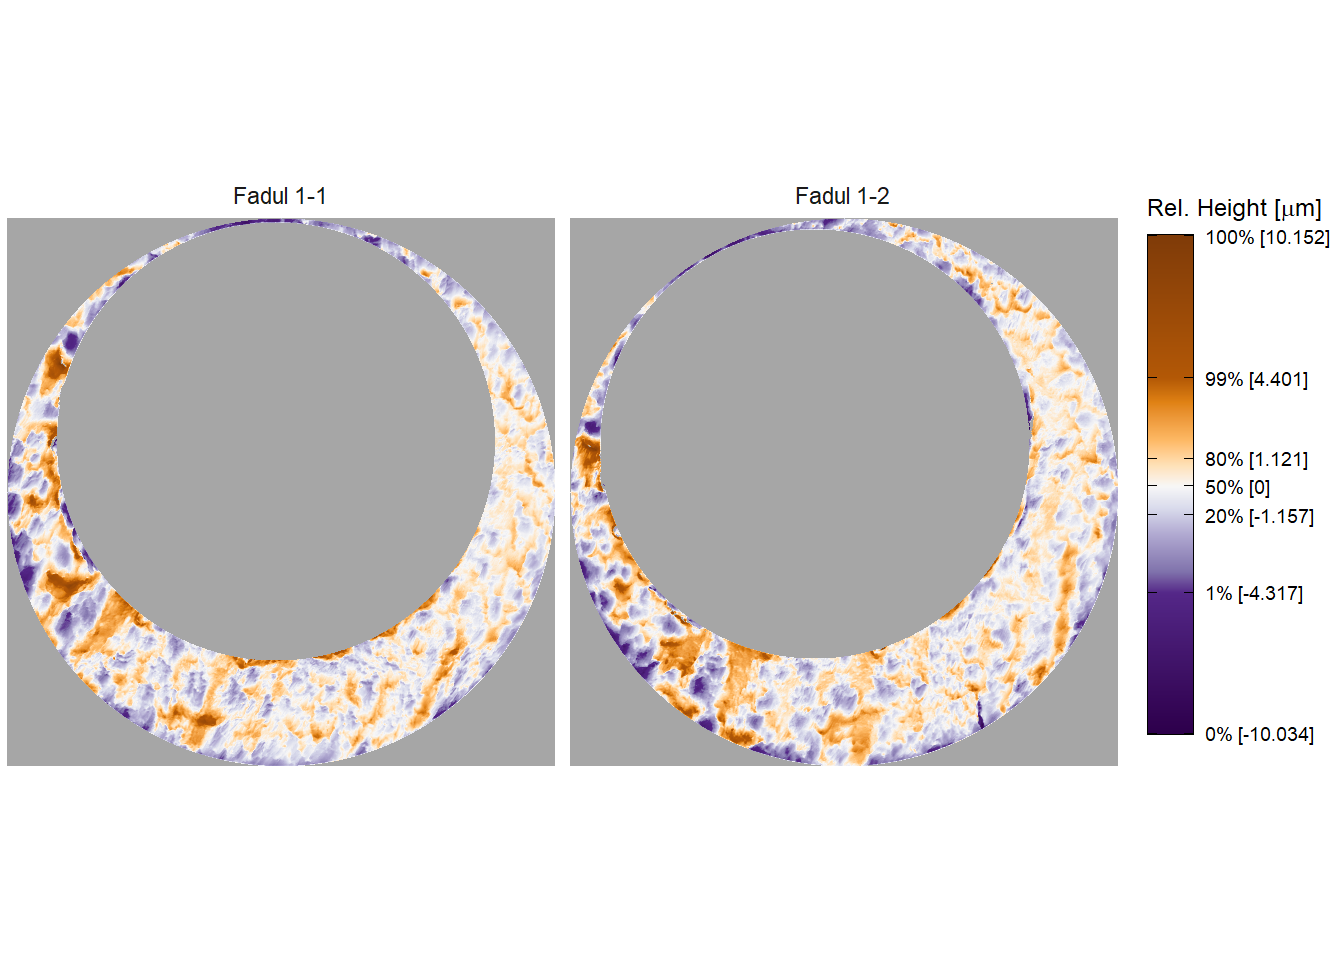
\includegraphics{thesis_files/figure-latex/processedScans-1} 

}

\caption{Fadul 1-1 and Fadul 1-2 after pre-processing. Similar striated markings are now easier to visually identify on both surfaces. It is now clearer that one of the scans needs to be rotated to align better with the other.}\label{fig:processedScans}
\end{figure}

\hypertarget{comparisonProcedure}{%
\subsection{``Correlation cell'' comparison procedure}\label{comparisonProcedure}}

As described in \citet{song_proposed_2013}, breech face markings are not uniformly impressed upon a cartridge case during the firing process.
As such, only certain sections of the cartridge case are used in a comparison.
In the CMC pipeline as proposed by \citet{song_proposed_2013} two scans are compared by partitioning one breech face scan into a grid of so-called ``correlation cells''.
These cells are compared individually to their best-matching counterpart on the other scan.
If a large proportion of these correlation cells are highly similar to their counterparts on the other breech face scan, this is considered as evidence that the markings on the two cartridge cases were made by the same source.
The number of highly similar cells is defined as the \emph{CMC count} \(C\) \citep{song_proposed_2013} of the breech-face comparison.
The CMC count is considered to be a more robust measure of similarity than the correlation calculated between two full scans.

\begin{figure}[htbp]

{\centering 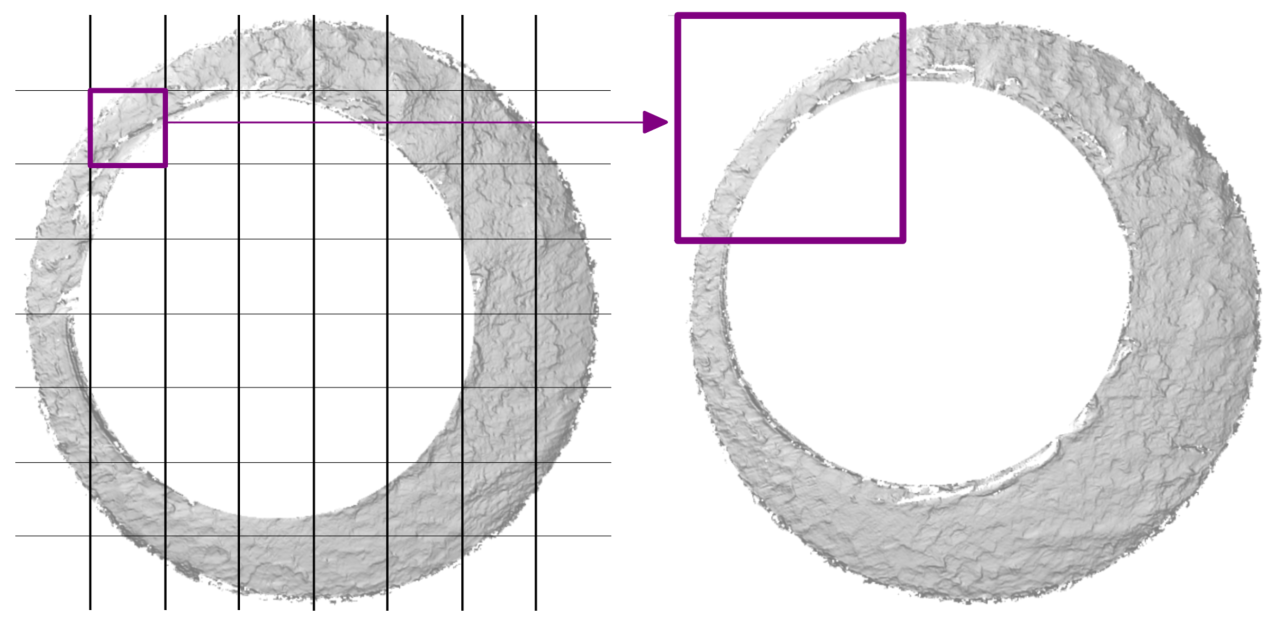
\includegraphics[width=.75\textwidth]{images/cmc_illustration} 

}

\caption{Illustration of comparing a cell in the reference cartridge case scan (left) to a larger region in a questioned cartridge case scan (right). Every one of the cells in the reference cartridge case is similarly paired with a region in the questioned cartridge case.  To determine the rotation at which the two cartridge cases align, the cell-region pairs are compared for various rotations of the questioned cartridge case.}\label{fig:cmc-illustration}
\end{figure}

Figure \ref{fig:cmc-illustration} illustrates the cell-based comparison procedure between two cartridge case scans.
The scan on the left serves as the reference; it is divided into a grid of \(8 \times 8\) cells.

\begin{figure}[!htbp]

{\centering 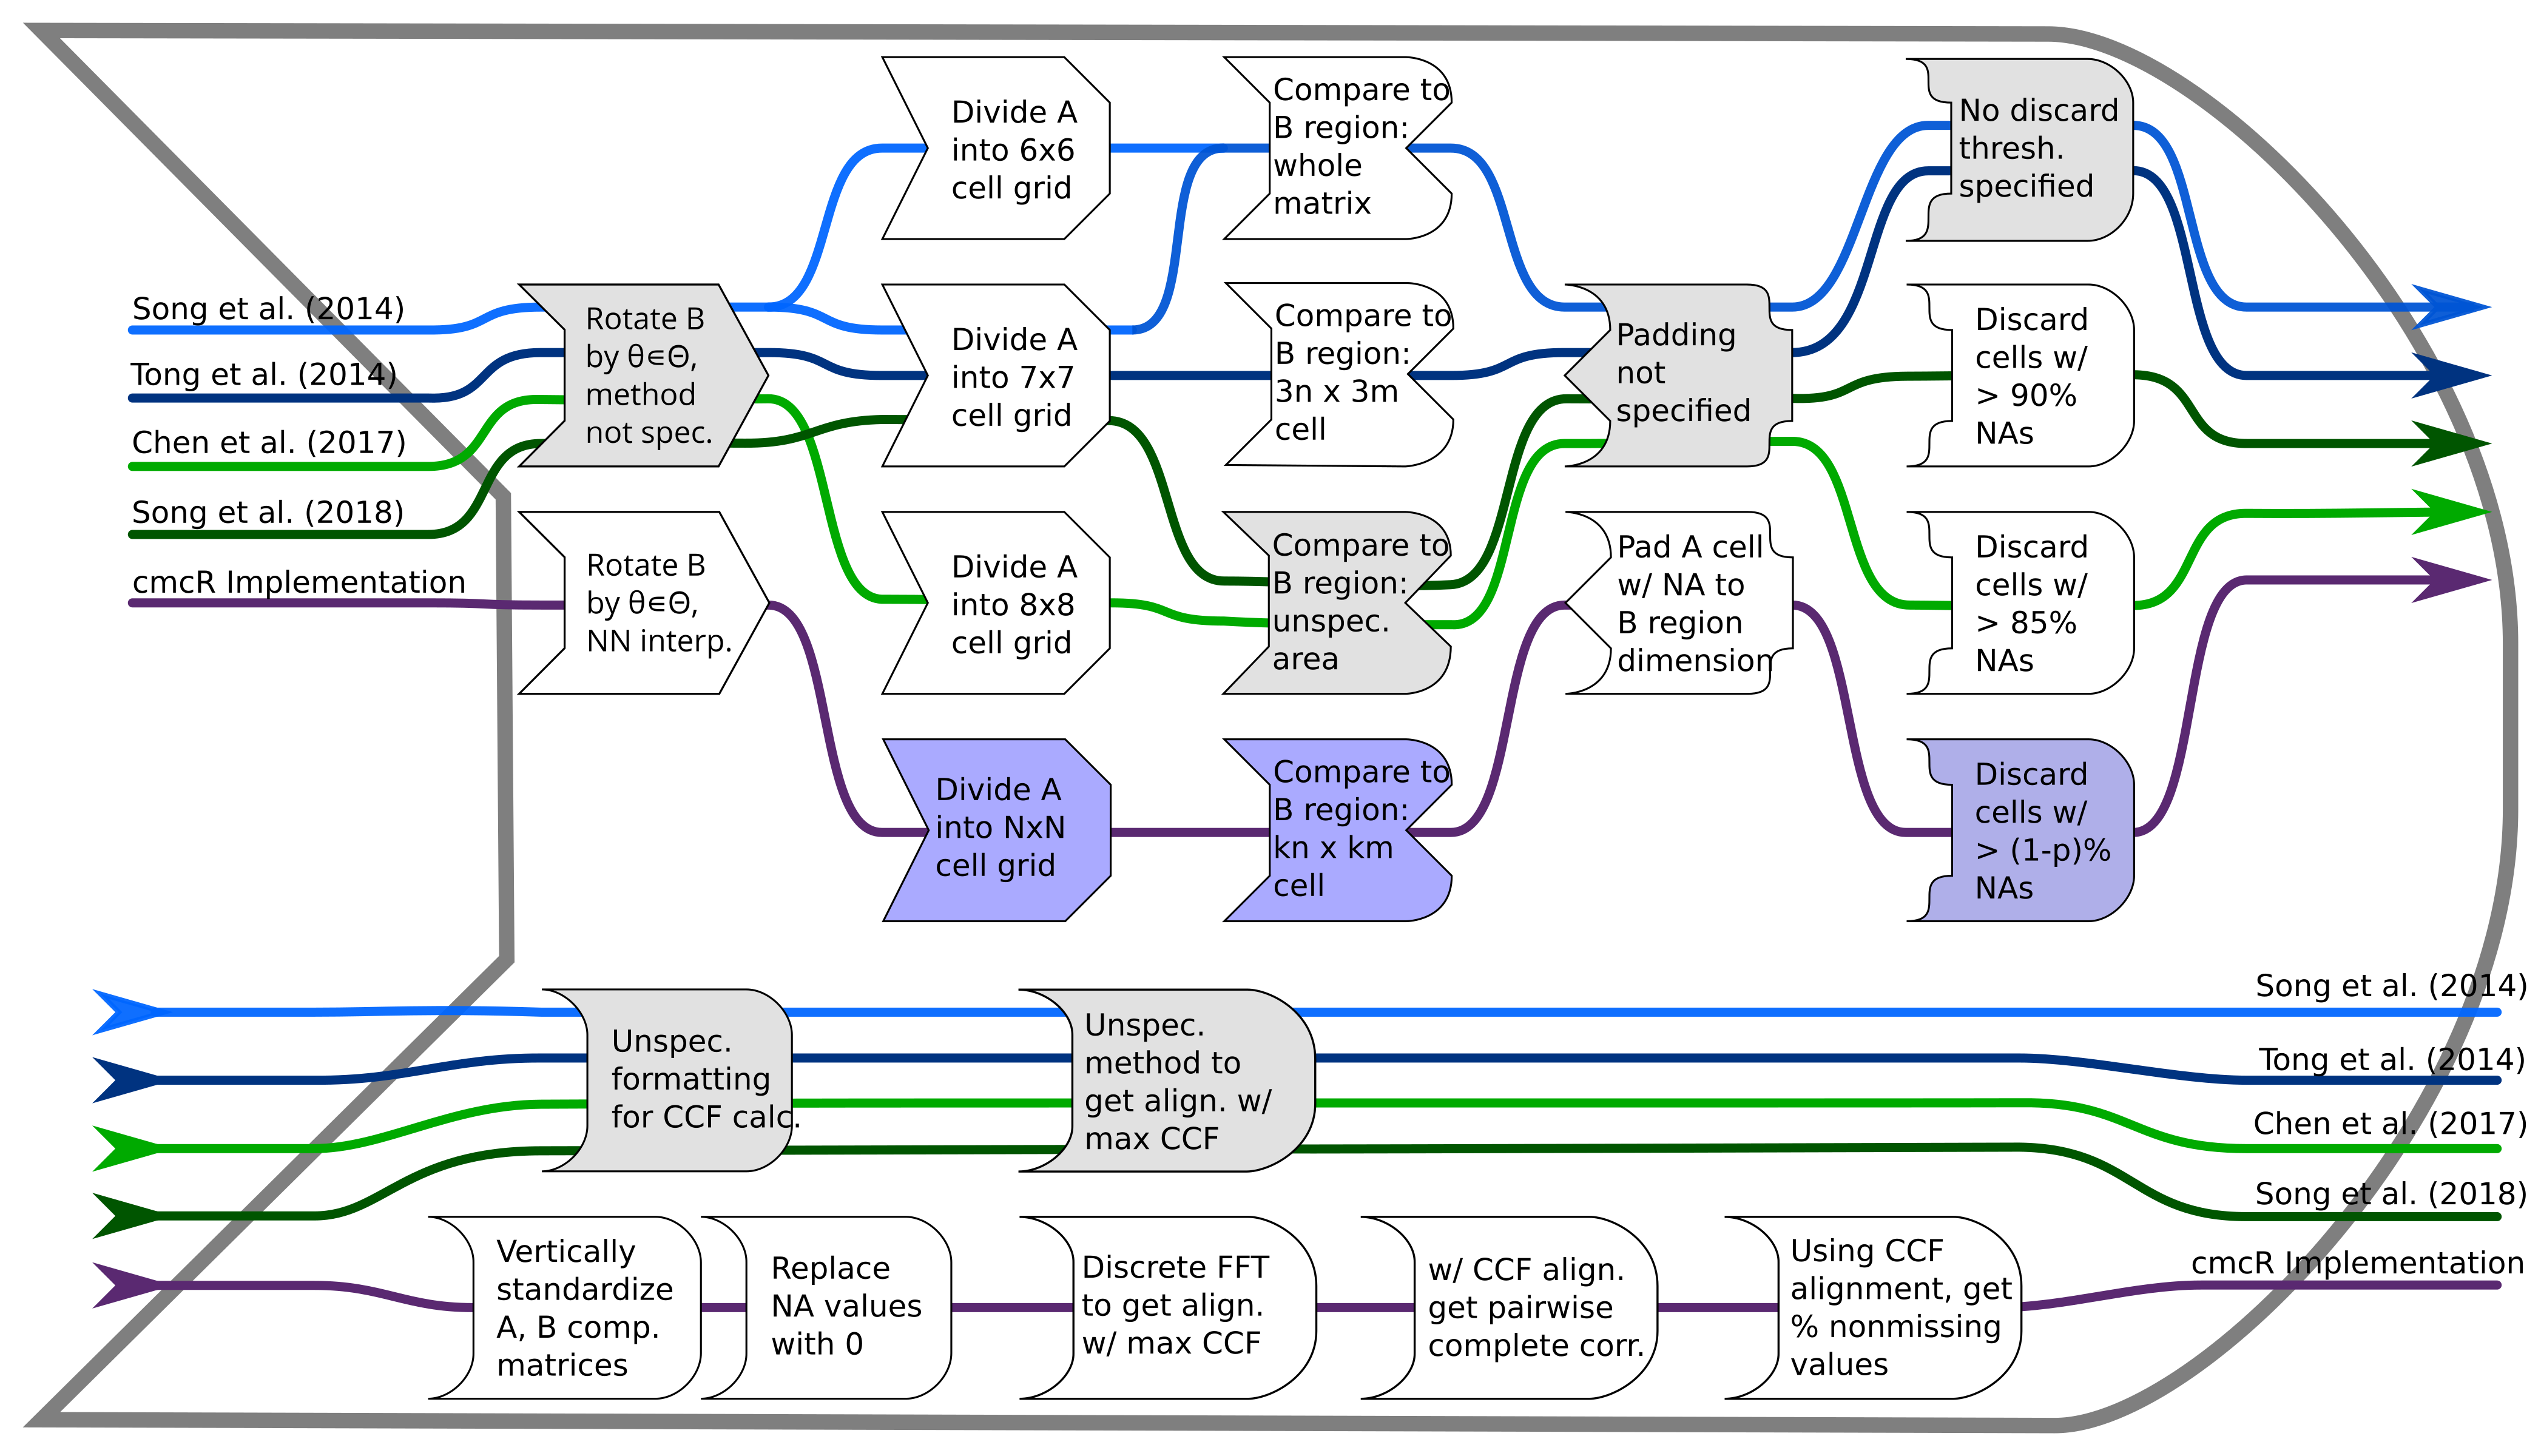
\includegraphics[width=58.17in]{images/cmc_flow} 

}

\caption{Each CMC implementation uses a slightly different procedure to obtain a similarity score between two cartridge cases. Steps which are implemented with additional user-specified parameters are shaded purple; steps which are described but without sufficient detail are shaded grey.}\label{fig:cmc-schematic}
\end{figure}

Figure \ref{fig:cmc-schematic} shows the steps of the correlation cell comparison process in each of the papers as well as the cmcR implementation.
Each cell is paired with an associated larger region in the other scan.
The absolute location of each cell and region in their respective surface matrices remain constant.
However, the scan on the right is rotated to determine the rotation at which the two scans are the most ``similar,'' as quantified by the \emph{cross-correlation function} (CCF).

For real-valued matrices \(A\) and \(B\) of dimension \(M \times N\) and \(P \times Q\), respectively, the cross-correlation function, denoted \((A \star B)\) is defined as
\[
(A \star B)[m,n] = \sum_{i=1}^M \sum_{j=1}^N A[i,j] B[(i + m), (j + n)],
\] where \(1 \leq m \leq M + P - 1\) and \(1 \leq n \leq N + Q - 1\).
By this definition, the \([m,n]\)th element of the resulting \(M + P - 1 \times N + Q - 1\) CCF matrix quantifies the similarity between matrices \(A\) and \(B\) for a translation of matrix \(B\) by \(m\) pixels horizontally and \(n\) pixel vertically.
The index at which the CCF attains a maximum represents the optimal translation needed to align \(B\) with \(A\).
The CCF as defined need not be bounded between \(-1\) and \(1\).
However, it is common to normalize the CCF for interpretability, and this is the convention adopted in the cmcR package.

Prior to calculating the CCF, the matrices \(A\) and \(B\) are standardized through subtraction of their respective means and division by their respective standard deviations.
This is referred to as the \emph{Areal Cross-Correlation Function} (ACCF) in some CMC papers \citep{ott_applying_2017}.
A direct calculation of the CCF for breech face scans based on the definition above is prohibitively slow.
While computationally feasible alternatives exist, \citet{song_proposed_2013} and other CMC papers do not specify the algorithm used to calculate the CCF.

Published descriptions of the CMC algorithm do not detail how the CCF is calculated.
In image processing, it is common to use an implementation based on the Fast Fourier Transform \citep{Brown1992}.
This implementation leverages the Cross-Correlation Theorem, which states that for matrices \(A\) and \(B\), the CCF can be expressed in terms of a frequency-domain pointwise product:
\[
(A \star B )[m,n]= \mathcal{F}^{-1}\left(\overline{\mathcal{F}(A)} \odot \mathcal{F}(B)\right)[m,n],
\]
where \(\mathcal{F}\) and \(\mathcal{F}^{-1}\) denote the discrete Fourier and inverse discrete Fourier transforms, respectively, and \(\overline{\mathcal{F}(A)}\) denotes the complex conjugate \citep{fft_brigham}.
Because the product on the right-hand side is calculated pointwise, we trade the moving sum computations from the definition of the CCF for two forward Fourier transformations, a pointwise product, and an inverse Fourier transformation.
The Fast Fourier Transform (FFT) algorithm can be used to reduce the computational load considerably.
Our implementation of this FFT-based CCF calculation is adapted from the cartridges3D package \citep{cartridges3D}.

No computational shortcut comes without some trade-offs, though, and this FFT-based CCF calculation is no different.
The FFT does not tolerate missing values, and breech faces are not continuous surfaces -- all of the white regions in Figure \ref{fig:cmc-illustration} correspond to missing values.
While it is unclear how the CCF is implemented in the CMC papers, the cmcR package adopts the following conventions:

\begin{itemize}
\item
  Only cells with a minimum proportion of non-missing pixels are assessed. This minimum threshold differs across CMC papers (15\% in \citet{chen_convergence_2017} vs.~10\% in \citet{song_estimating_2018}, as shown in Figure \ref{fig:cmc-schematic}), and is referenced but not specified in several other papers \citep{tong_fired_2014, song_3d_2014, chu_validation_2013}. The \texttt{comparison\_calcPropMissing} function computes the proportion of a matrix that is missing (\texttt{NA}-valued).
\item
  Missing values are replaced with the overall mean value when the FFT-based CCF is computed (using function \texttt{comparison\_replaceMissing}).
\item
  The optimal translation is determined using the FFT-based CCF (using \texttt{comparison\_fft\_ccf}).
\item
  Based on the optimal translation determined from the FFT-based CCF, we compute the pairwise complete CCF directly, avoiding any distortion of the CCF computation based on compensation for missing values (using function \texttt{comparison\_cor}).
\end{itemize}

All of the steps dealing with cell-based comparisons are implemented as functions of the form \texttt{comparison\_*}.
Similar to the \texttt{preProcess\_*} functions, the \texttt{comparison\_*} functions can be chained together through a sequence of pipes.
Below, we use the \texttt{comparison\_allTogether} function to perform the entire cell-based comparison procedure in one call.
The comparison procedure is performed twice: once with Fadul 1-1 considered the ``reference'' scan divided into cells that are compared to the ``target'' scan Fadul 1-2 and again with the roles reversed.

\begin{Shaded}
\begin{Highlighting}[]
\CommentTok{\# Fill in most of the arguments first}
\NormalTok{comp\_w\_pars }\OtherTok{\textless{}{-}}\NormalTok{ purrr}\SpecialCharTok{::}\FunctionTok{partial}\NormalTok{(}\AttributeTok{.f =}\NormalTok{ comparison\_allTogether,}
                              \AttributeTok{numCells =} \FunctionTok{c}\NormalTok{(}\DecValTok{8}\NormalTok{,}\DecValTok{8}\NormalTok{), }\AttributeTok{maxMissingProp =}\NormalTok{ .}\DecValTok{85}\NormalTok{)}

\CommentTok{\# Then, map the remaining values to theta}
\NormalTok{kmComparisonFeatures }\OtherTok{\textless{}{-}}\NormalTok{ purrr}\SpecialCharTok{::}\FunctionTok{map\_dfr}\NormalTok{(}
  \FunctionTok{seq}\NormalTok{(}\SpecialCharTok{{-}}\DecValTok{30}\NormalTok{,}\DecValTok{30}\NormalTok{,}\AttributeTok{by =} \DecValTok{3}\NormalTok{),}
  \SpecialCharTok{\textasciitilde{}}\FunctionTok{comp\_w\_pars}\NormalTok{(}\AttributeTok{reference =}\NormalTok{ fadul1}\FloatTok{.1}\NormalTok{, }\AttributeTok{target =}\NormalTok{ fadul1}\FloatTok{.2}\NormalTok{, }\AttributeTok{theta =}\NormalTok{ .))}

\NormalTok{kmComparisonFeatures\_rev }\OtherTok{\textless{}{-}}\NormalTok{ purrr}\SpecialCharTok{::}\FunctionTok{map\_dfr}\NormalTok{(}
  \FunctionTok{seq}\NormalTok{(}\SpecialCharTok{{-}}\DecValTok{30}\NormalTok{,}\DecValTok{30}\NormalTok{,}\AttributeTok{by =} \DecValTok{3}\NormalTok{),}
  \SpecialCharTok{\textasciitilde{}}\FunctionTok{comp\_w\_pars}\NormalTok{(}\AttributeTok{reference =}\NormalTok{ fadul1}\FloatTok{.2}\NormalTok{, }\AttributeTok{target =}\NormalTok{ fadul1}\FloatTok{.1}\NormalTok{, }\AttributeTok{theta =}\NormalTok{ .))}
\end{Highlighting}
\end{Shaded}

The \texttt{comparison\_allTogether} function consists of the following steps wrapped into a single convenience function:

\begin{itemize}
\tightlist
\item
  \texttt{comparison\_cellDivision}: Divide the reference scan into cells
\item
  \texttt{comparison\_getTargetRegions}: Extract regions associated with each reference cell from the target scan
\item
  \texttt{comparison\_calcPropMissing}: Compute missing proportions and filter out cells with a proportion of missing values above the threshold.
\item
  \texttt{comparison\_standardizeHeights}: Standardize height values
\item
  \texttt{comparison\_replaceMissing}: Replace missing values
\item
  \texttt{comparison\_fft\_ccf}: Compute CCF and estimated translations using FFT
\item
  \texttt{comparison\_alignedTargetCell}: Extract a matrix from the target scan corresponding to the region of the target scan to which the reference cell aligns
\item
  \texttt{cor}: Calculate the pairwise-complete correlation between each cell pair
\end{itemize}

The \texttt{comparison\_allTogether} is called repeatedly while rotating the target scan by a set of rotation angles.
When implementing the High CMC decision rule \citep{tong_improved_2015}, both combinations of reference and target scan are examined (e.g.~A-B and B-A).

Table \ref{tab:cellCCF-latex} shows several rows of the data frame output of the \texttt{comparison\_allTogether} function for the comparison of Fadul 1-1 vs.~Fadul 1-2 considering Fadul 1-1 as the reference scan.
Although we used a grid of \(8 \times 8\) cells, there were only 26 cell-region pairs that contained a sufficient proportion of non-missing values (15\% in this example).
The features derived from the correlation cell procedure (CCF\(_{max}\), \(\Delta x\), \(\Delta y\), \(\theta\)) are then used to measure the similarity between scans.

\begin{table}

\caption{\label{tab:cellCCF-latex}Example of output from correlation cell comparison procedure between Fadul 1-1 and Fadul 1-2 rotated by -24 degrees. Due to the large proportion of missing values that are replaced to compute the FFT-based correlation, the pairwise-complete correlation is most often greater than the FFT-based correlation.}
\centering
\begin{tabu} to \linewidth {>{\raggedright}X>{\raggedleft}X>{\raggedleft}X>{\raggedleft}X>{\raggedleft}X>{\raggedleft}X}
\toprule
\textbf{Cell Index} & \textbf{Pairwise-comp. corr.} & \textbf{FFT-based corr.} & \textbf{$\Delta$x} & \textbf{$\Delta$y} & \textbf{$\theta$}\\
\midrule
2, 7 & 0.432 & 0.228 & -14 & -33 & -24\\
2, 8 & 0.464 & 0.176 & 9 & -44 & -24\\
3, 1 & 0.841 & 0.478 & -7 & 15 & -24\\
3, 8 & 0.699 & 0.277 & -7 & 5 & -24\\
4, 1 & 0.850 & 0.375 & -4 & 11 & -24\\
\bottomrule
\end{tabu}
\end{table}

\hypertarget{decision-rule}{%
\subsection{Decision rule}\label{decision-rule}}

For each cell on the reference scan, we calculate the translation \((\Delta x, \Delta y)\) and cross-correlation across rotations by a set of angles \(\theta\) of the target scan.
The task is to determine whether multiple cells come to a ``consensus'' on a particular translation and rotation.
If such a consensus is reached, then there is evidence that a true aligning translation and rotation exists and the cartridge cases match.
The CMC decision rules principally differ in how they identify consensus among the \(\Delta x, \Delta y, \theta\) values.
Here, we describe the two pipelines implemented in the cmcR package: using the original decision rule described in \citet{song_3d_2014} and the High CMC decision rule proposed in \citet{tong_improved_2015}.

\hypertarget{originalMethod}{%
\subsubsection{The Original CMC decision rule}\label{originalMethod}}

This section briefly describes the decision rule used in the first CMC paper \citep{song_proposed_2013}.
For a thorough explanation of the procedure, refer to the \href{https://csafe-isu.github.io/cmcR/articles/decisionRuleDescription.html}{CMC Decision Rule Description} vignette of the cmcR package.

Let \(x_i, y_i, \theta_i\) denote the translation and rotation parameters which produce the highest CCF for the alignment of cell-region pair \(i\), \(i = 1,...,n\) where \(n\) is the total number of cell-region pairs containing a sufficient proportion of non-missing values.
\citet{song_proposed_2013} propose the median as a consensus \((x_{\text{ref}}, y_{\text{ref}}, \theta_{\text{ref}})\) across the cell-region pairs.
Then, the distance between each \((x_i, y_i, \theta_i)\) and \((x_{\text{ref}}, y_{\text{ref}}, \theta_{\text{ref}})\) is compared to thresholds \(T_{x}, T_{y}, T_\theta, T_{\text{CCF}}\).
A cell-region pair \(i\) is declared a ``match'' if all of the following conditions hold:

\begin{eqnarray}
|x_i - x_{\text{ref}}| &\leq& T_{x}, \\ \nonumber
|y_i - y_{\text{ref}}| &\leq& T_{y}, \\ \nonumber
|\theta_i - \theta_{\text{ref}}| &\leq& T_{\theta}, \\ \nonumber
\text{CCF}_{\max,i} &\geq& T_{\text{CCF}}.
\label{eq:original}
\end{eqnarray}

The number of matching cell-region pairs, the ``CMC count,'' is used as a measure of similarity between the two cartridge cases.
\citet{song_3d_2014} indicate that the thresholds \(T_{x}, T_{y}, T_\theta, T_{\text{CCF}}\) need to be determined experimentally.
Table \ref{tab:thresholdTable-latex} summarizes the thresholds used in various CMC papers.

\begin{table}

\caption{\label{tab:thresholdTable-latex}Different thresholds for translation, rotation, and CCF$_{\max}$ are used across different papers. The range in CCF$_{\max}$ is particularly notable.}
\centering
\begin{tabu} to \linewidth {>{\raggedright}X>{\raggedleft}X>{\raggedleft}X>{\raggedleft}X}
\toprule
\textbf{Paper} & \textbf{Translation $T_x, T_y$ (in pixels)} & \textbf{Rotation $\theta$ (in degrees)} & \textbf{$CCF_{\max}$}\\
\midrule
Song et al. (2014) & 20 & 6 & 0.60\\
Tong et al. (2014) & 30 & 3 & 0.25\\
Tong et al. (2015) & 15 & 3 & 0.55\\
Chen et al. (2017) & 20 & 3 & 0.40\\
Song et al. (2018) & 20 & 6 & 0.50\\
\bottomrule
\end{tabu}
\end{table}

Unlike the original CMC pipeline, the High CMC decision rule considers multiple rotations for each cell-region pair.

\hypertarget{highCMCMethod}{%
\subsubsection{The High CMC decision rule}\label{highCMCMethod}}

For the High CMC decision rule, two scans are compared in both directions - i.e., each scan takes on the role of the reference scan that is partitioned into a grid of cells.
\citet{tong_improved_2015} claim that some matching cell-region pairs ``may be mistakenly excluded from the CMC count'' under the original decision rule because they attain the largest CCF at a rotation outside the range allowed by \(T_\theta\) ``by chance.''

\citet{tong_improved_2015} introduce consensus values across all cell-region pairs for each rotation angle \(\theta\) and calculate a \(\theta\)-dependent CMC count as the sum of matches observed.
Under the High CMC rule, a cell-region pair \(i\) is defined as a match conditional on a particular rotation \(\theta\) if it satisfies the following three conditions:

\begin{eqnarray}
|x_{i,\theta} - x_{ref,\theta}| &\leq& T_x \\ \nonumber
|y_{i,\theta} - y_{ref,\theta}| &\leq& T_y \\ \nonumber
\text{CCF}_{i,\theta} &\geq& T_{\text{CCF}}.
\label{eq:highCMC}
\end{eqnarray}

The \(\theta\)-dependent CMC count, CMC\(_\theta\), is defined as the sum of matching cell-region pairs.

\citet{tong_improved_2015} assert that for a truly matching cartridge case pair, the relationship between \(\theta\) and CMC\(_\theta\) should exhibit a ``prominent peak'' near the true rotation value.
That is, CMC\(_{\theta}\) should be largest when the scans are close to being correctly aligned.
Further, non-matching pairs should exhibit a ``relatively flat and random {[}\ldots{]} pattern'' across the CMC\(_{\theta}\) values.

To determine whether a ``prominent peak'' exists in the relationship between \(\theta\) and CMC\(_\theta\), \citet{tong_improved_2015} consider an interval of rotation angles with large associated CMC\(_\theta\) values.
Let \(CMC_{\text{max}} = \max_{\theta} CMC_{\theta}\) be the maximum CMC\(_\theta\) count across all rotation angles.
For \(\tau > 0\), define \(S(\tau) = \{\theta : CMC_\theta > (CMC_{\max} - \tau)\}\) as the set of rotations with ``large'' CMC\(_\theta\) values.
\citet{tong_improved_2015} consider the ``angular range'' as \(R(\tau) = |\max_{\theta} S(\tau) - \min_\theta S(\tau)|\).
If \(R(\tau)\) is small, then there is evidence that many cells agree on a single rotation and that the scans match.
To arrive at a CMC count similarity score, \citet{tong_improved_2015} suggest a value for \(\tau\) of 1 and determine:

\begin{quote}
If the angular range of the ``high CMCs'' is within the range \(T_\theta\), identify the CMCs for each rotation angle in this range and combine them to give the number of CMCs for this comparison in place of the original CMC number.
\end{quote}

If the angular range is larger than \(T_\theta\), we say that the cartridge case pair ``fails'' the High CMC criteria and the original CMC number is used.
The High CMC decision rule returns a CMC count at least as large as the original decision rule.

\hypertarget{decisionRuleImplementation}{%
\subsubsection{Implementation of decision rules}\label{decisionRuleImplementation}}

In this section, we implement the decision rules in cmcR for both the original and High CMC decision rules.
For illustrative purposes, we consider a set of thresholds: \(T_x = T_y = 20\), \(T_{\theta} = 6\), and \(T_{\text{CCF}} = 0.5\).

Decision rules in cmcR are implemented as functions of the form \texttt{decision\_*}.
In particular, the \texttt{decision\_CMC} function applies both the original and High CMC decision rules depending on if the parameter \(\tau\) is set.
The code below demonstrates the use of \texttt{decision\_CMC} on the features \texttt{kmComparisonFeatures}, extracted from the comparison of scans Fadul 1-1 vs.~Fadul 1-2.
Conversely, \texttt{kmComparisonFeatures\_rev} contains the features from a comparison of Fadul 1-2 vs.~Fadul 1-1.
For comparison, we also compute the CMCs under both decision rules for the comparison between the non-match pair Fadul 1-1 and Fadul 2-1 (not shown to avoid redundancy).

\begin{Shaded}
\begin{Highlighting}[]
\NormalTok{kmComparison\_cmcs }\OtherTok{\textless{}{-}}\NormalTok{ kmComparisonFeatures }\SpecialCharTok{\%\textgreater{}\%} \FunctionTok{mutate}\NormalTok{(}
  \AttributeTok{originalMethodClassif =}
    \FunctionTok{decision\_CMC}\NormalTok{(}\AttributeTok{cellIndex =}\NormalTok{ cellIndex, }\AttributeTok{x =}\NormalTok{ x, }\AttributeTok{y =}\NormalTok{ y, }\AttributeTok{theta =}\NormalTok{ theta,}
                 \AttributeTok{corr =}\NormalTok{ pairwiseCompCor, }\AttributeTok{xThresh =} \DecValTok{20}\NormalTok{, }\AttributeTok{thetaThresh =} \DecValTok{6}\NormalTok{,}
                 \AttributeTok{corrThresh =}\NormalTok{ .}\DecValTok{5}\NormalTok{),}
  \AttributeTok{highCMCClassif =}
    \FunctionTok{decision\_CMC}\NormalTok{(}\AttributeTok{cellIndex =}\NormalTok{ cellIndex, }\AttributeTok{x =}\NormalTok{ x, }\AttributeTok{y =}\NormalTok{ y, }\AttributeTok{theta =}\NormalTok{ theta,}
                 \AttributeTok{corr =}\NormalTok{ pairwiseCompCor, }\AttributeTok{xThresh =} \DecValTok{20}\NormalTok{, }\AttributeTok{thetaThresh =} \DecValTok{6}\NormalTok{,}
                 \AttributeTok{corrThresh =}\NormalTok{ .}\DecValTok{5}\NormalTok{, }\AttributeTok{tau =} \DecValTok{1}\NormalTok{))}
\end{Highlighting}
\end{Shaded}

We use the \texttt{cmcPlot} function to visualize congruent matching cells (CMCs) and non-congruent matching cells (non-CMCs).
Figure \ref{fig:topVoteCMCPlot} shows the CMCs and non-CMCs in blue and red, respectively, based on the original decision rule.
The (red) non-CMC patches are shown in the position where the maximum CCF value in the target scan is attained.
The top row shows 18 CMCs in blue and 8 non-CMCs in red when Fadul 1-1 is treated as the reference and Fadul 1-2 the target.
The bottom row shows the 17 CMCs and 13 non-CMCs when the roles are reversed.
There is no discussion in \citet{song_proposed_2013} about combining the results from these two comparison directions, but \citet{tong_improved_2015} propose using the minimum of the two CMC counts (17 in this example).

\begin{figure}[htbp]

{\centering 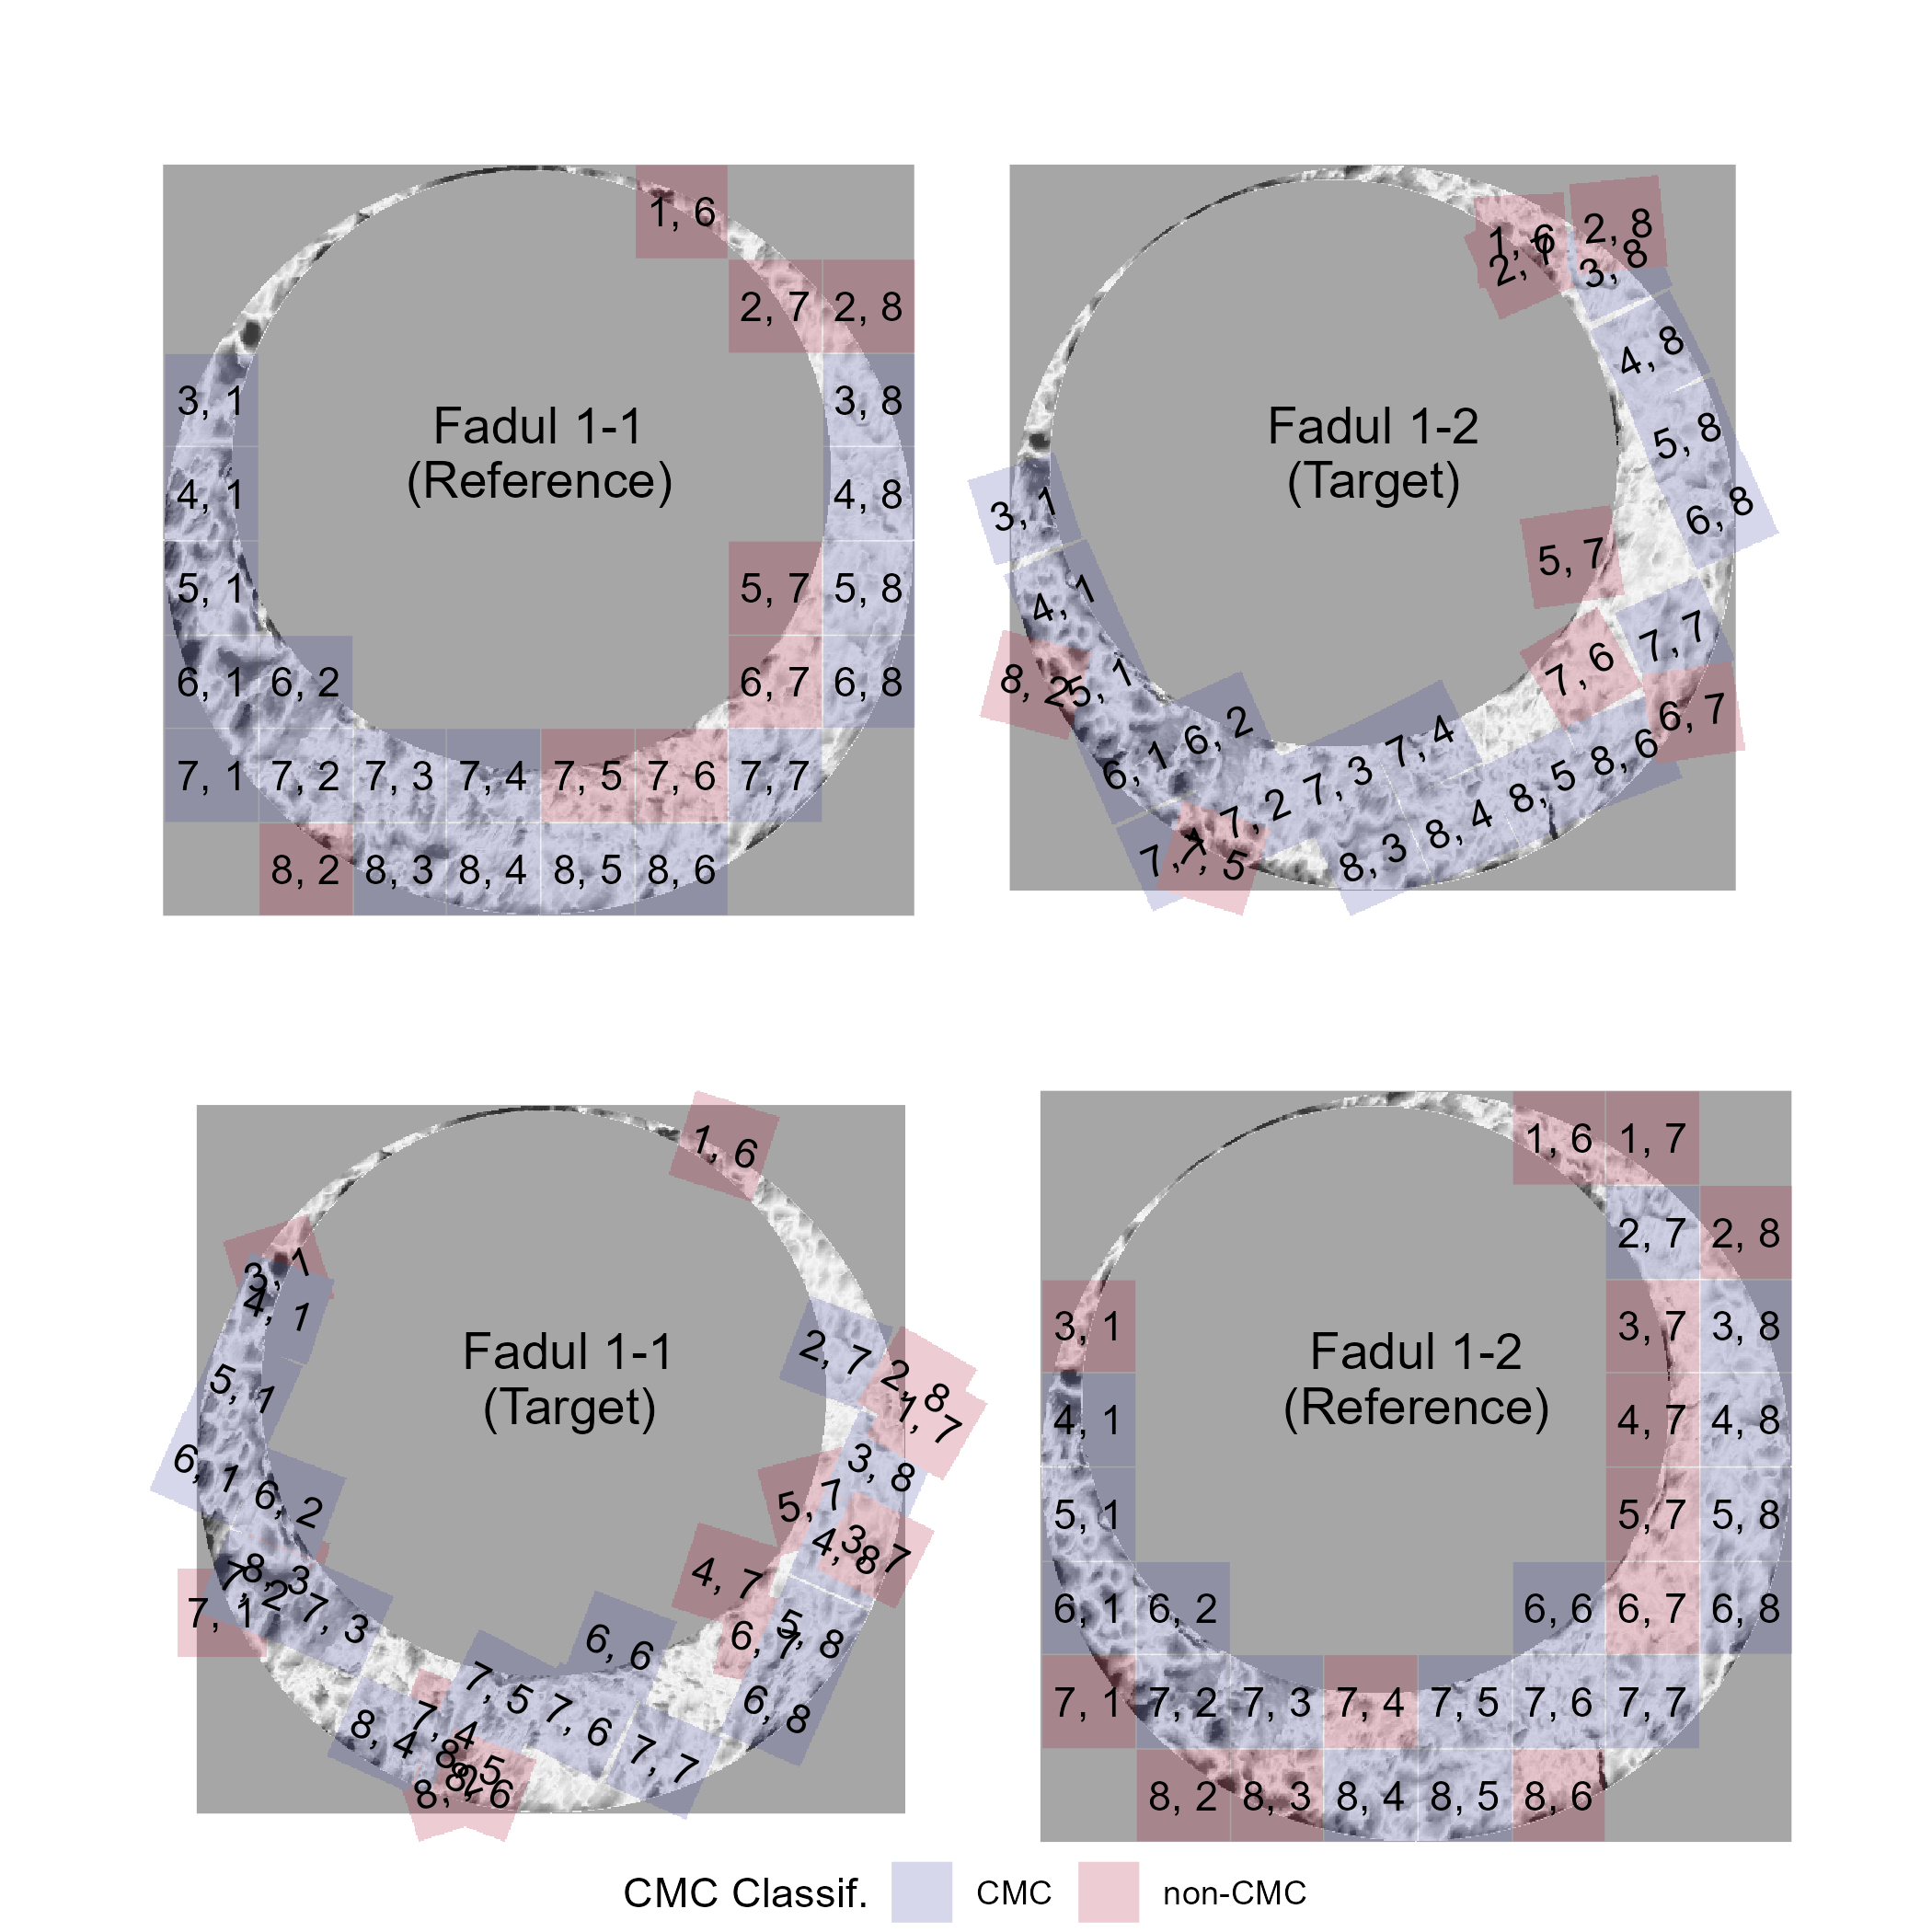
\includegraphics[width=29.17in]{figures/kmOriginalMethod} 

}

\caption{CMC results for the comparison between Fadul 1-1 and Fadul 1-2 using the original decision rule. The two plots in the top row show the 18 CMCs when Fadul 1-1 is treated as the "reference" cartridge case to which Fadul 1-2 (the "target") is compared. The second row shows the 17 CMCs when the roles are reversed. Red cells indicate where cells not identified as congruent achieve the maximum pairwise-complete correlation across all rotations of the target scan.}\label{fig:topVoteCMCPlot}
\end{figure}

Similarly, CMCs and non-CMCs determined under the High CMC decision rule are shown in Figure \ref{fig:highCMCPlot}.
Treating Fadul 1-1 and Fadul 1-2 as the reference scan yields 20 and 18 CMCs, respectively.
Combining the results as described above, the final High CMC count is 24.

\begin{figure}[htbp]

{\centering 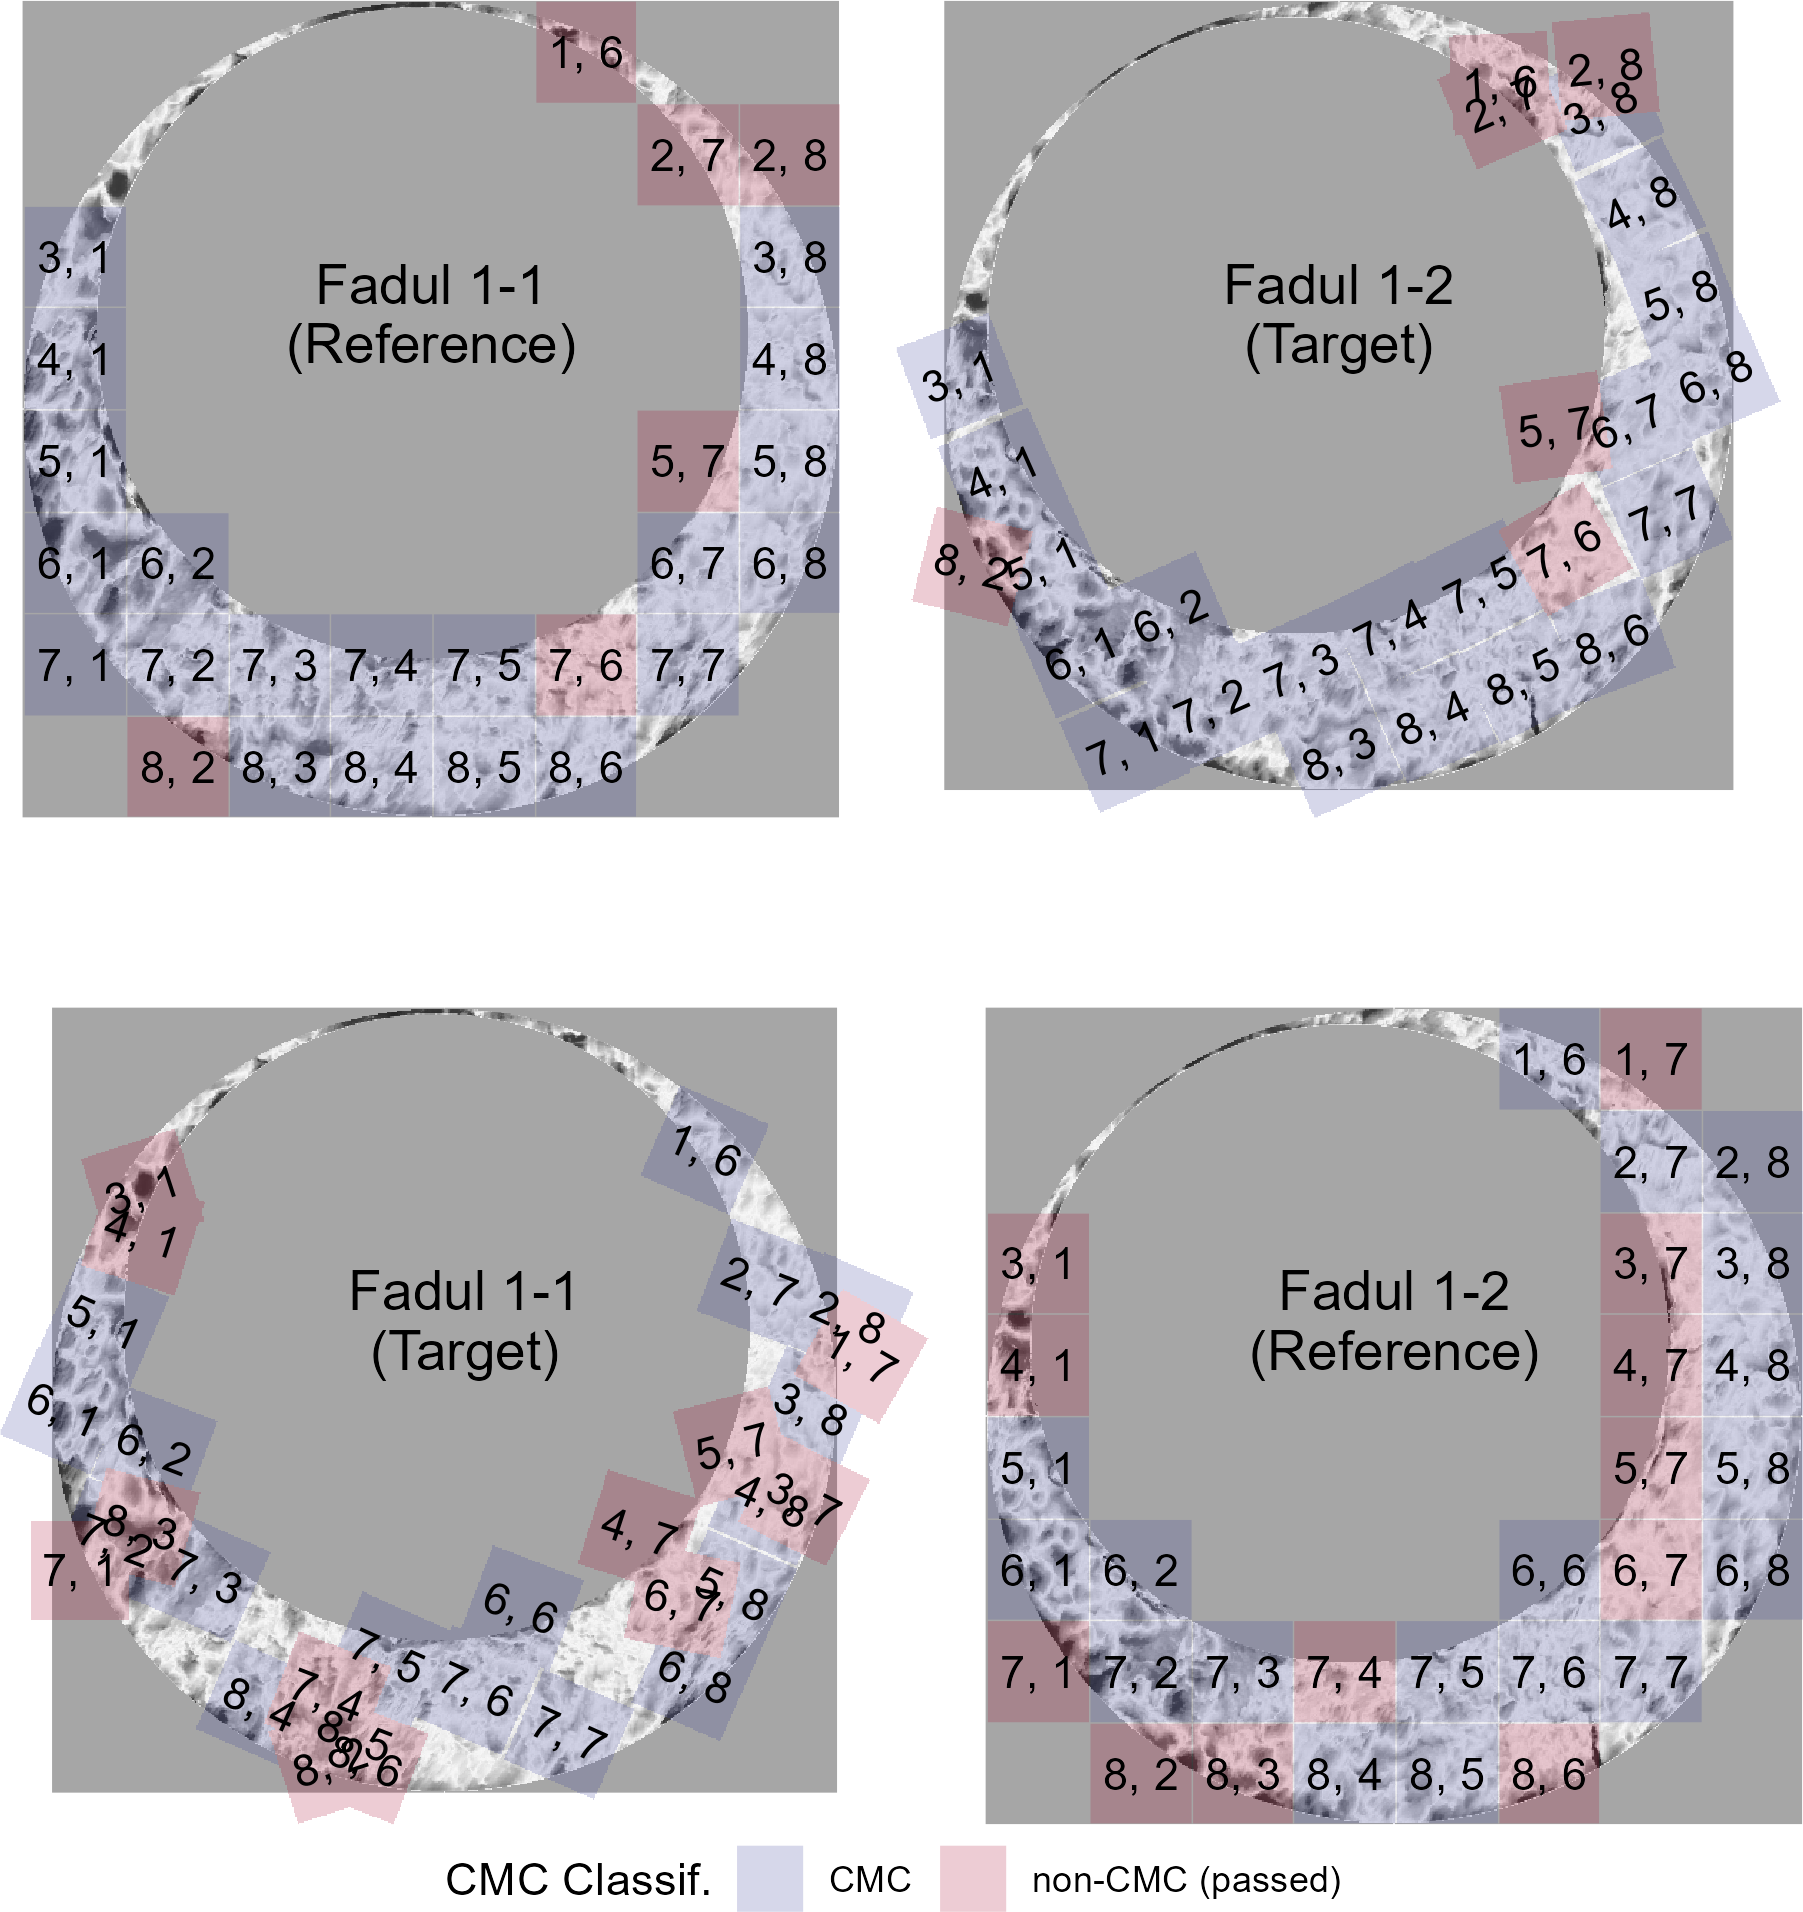
\includegraphics[width=29.17in]{figures/kmHighCMC} 

}

\caption{Applying the High CMC decision rule to the comparison of Fadul 1-1 and Fadul 1-2 results in 20 CMCs when Fadul 1-1 is treated as the reference (top) and 18 CMCs when Fadul 1-2 is treated as the reference (bottom). Although the individual comparisons do not yield considerably more CMCs than under the original CMC pipeline, Tong et al. (2015) indicate that the High CMCs from both comparisons are combined as the final High CMC count (each cell is counted at most once). Combining the results means that the High CMC decision rule tends to produce higher CMC counts than the original CMC pipeline. In this example, the combined High CMC count is 24 CMCs.}\label{fig:highCMCPlot}
\end{figure}

In contrast, Figure \ref{fig:knmCMCPlot} shows the CMC results for a comparison between Fadul 1-1 and a known non-match scan, Fadul 2-1, under the exact same processing conditions.
Only two cells are classified as congruent matching cells under the original decision rule when Fadul 1-1 is the reference scan.
No cells are classified as CMCs in the other direction.
While not shown, this pair fails the High CMC criteria and thus was assigned 0 CMCs under the High CMC decision rule.

\begin{figure}[htbp]

{\centering 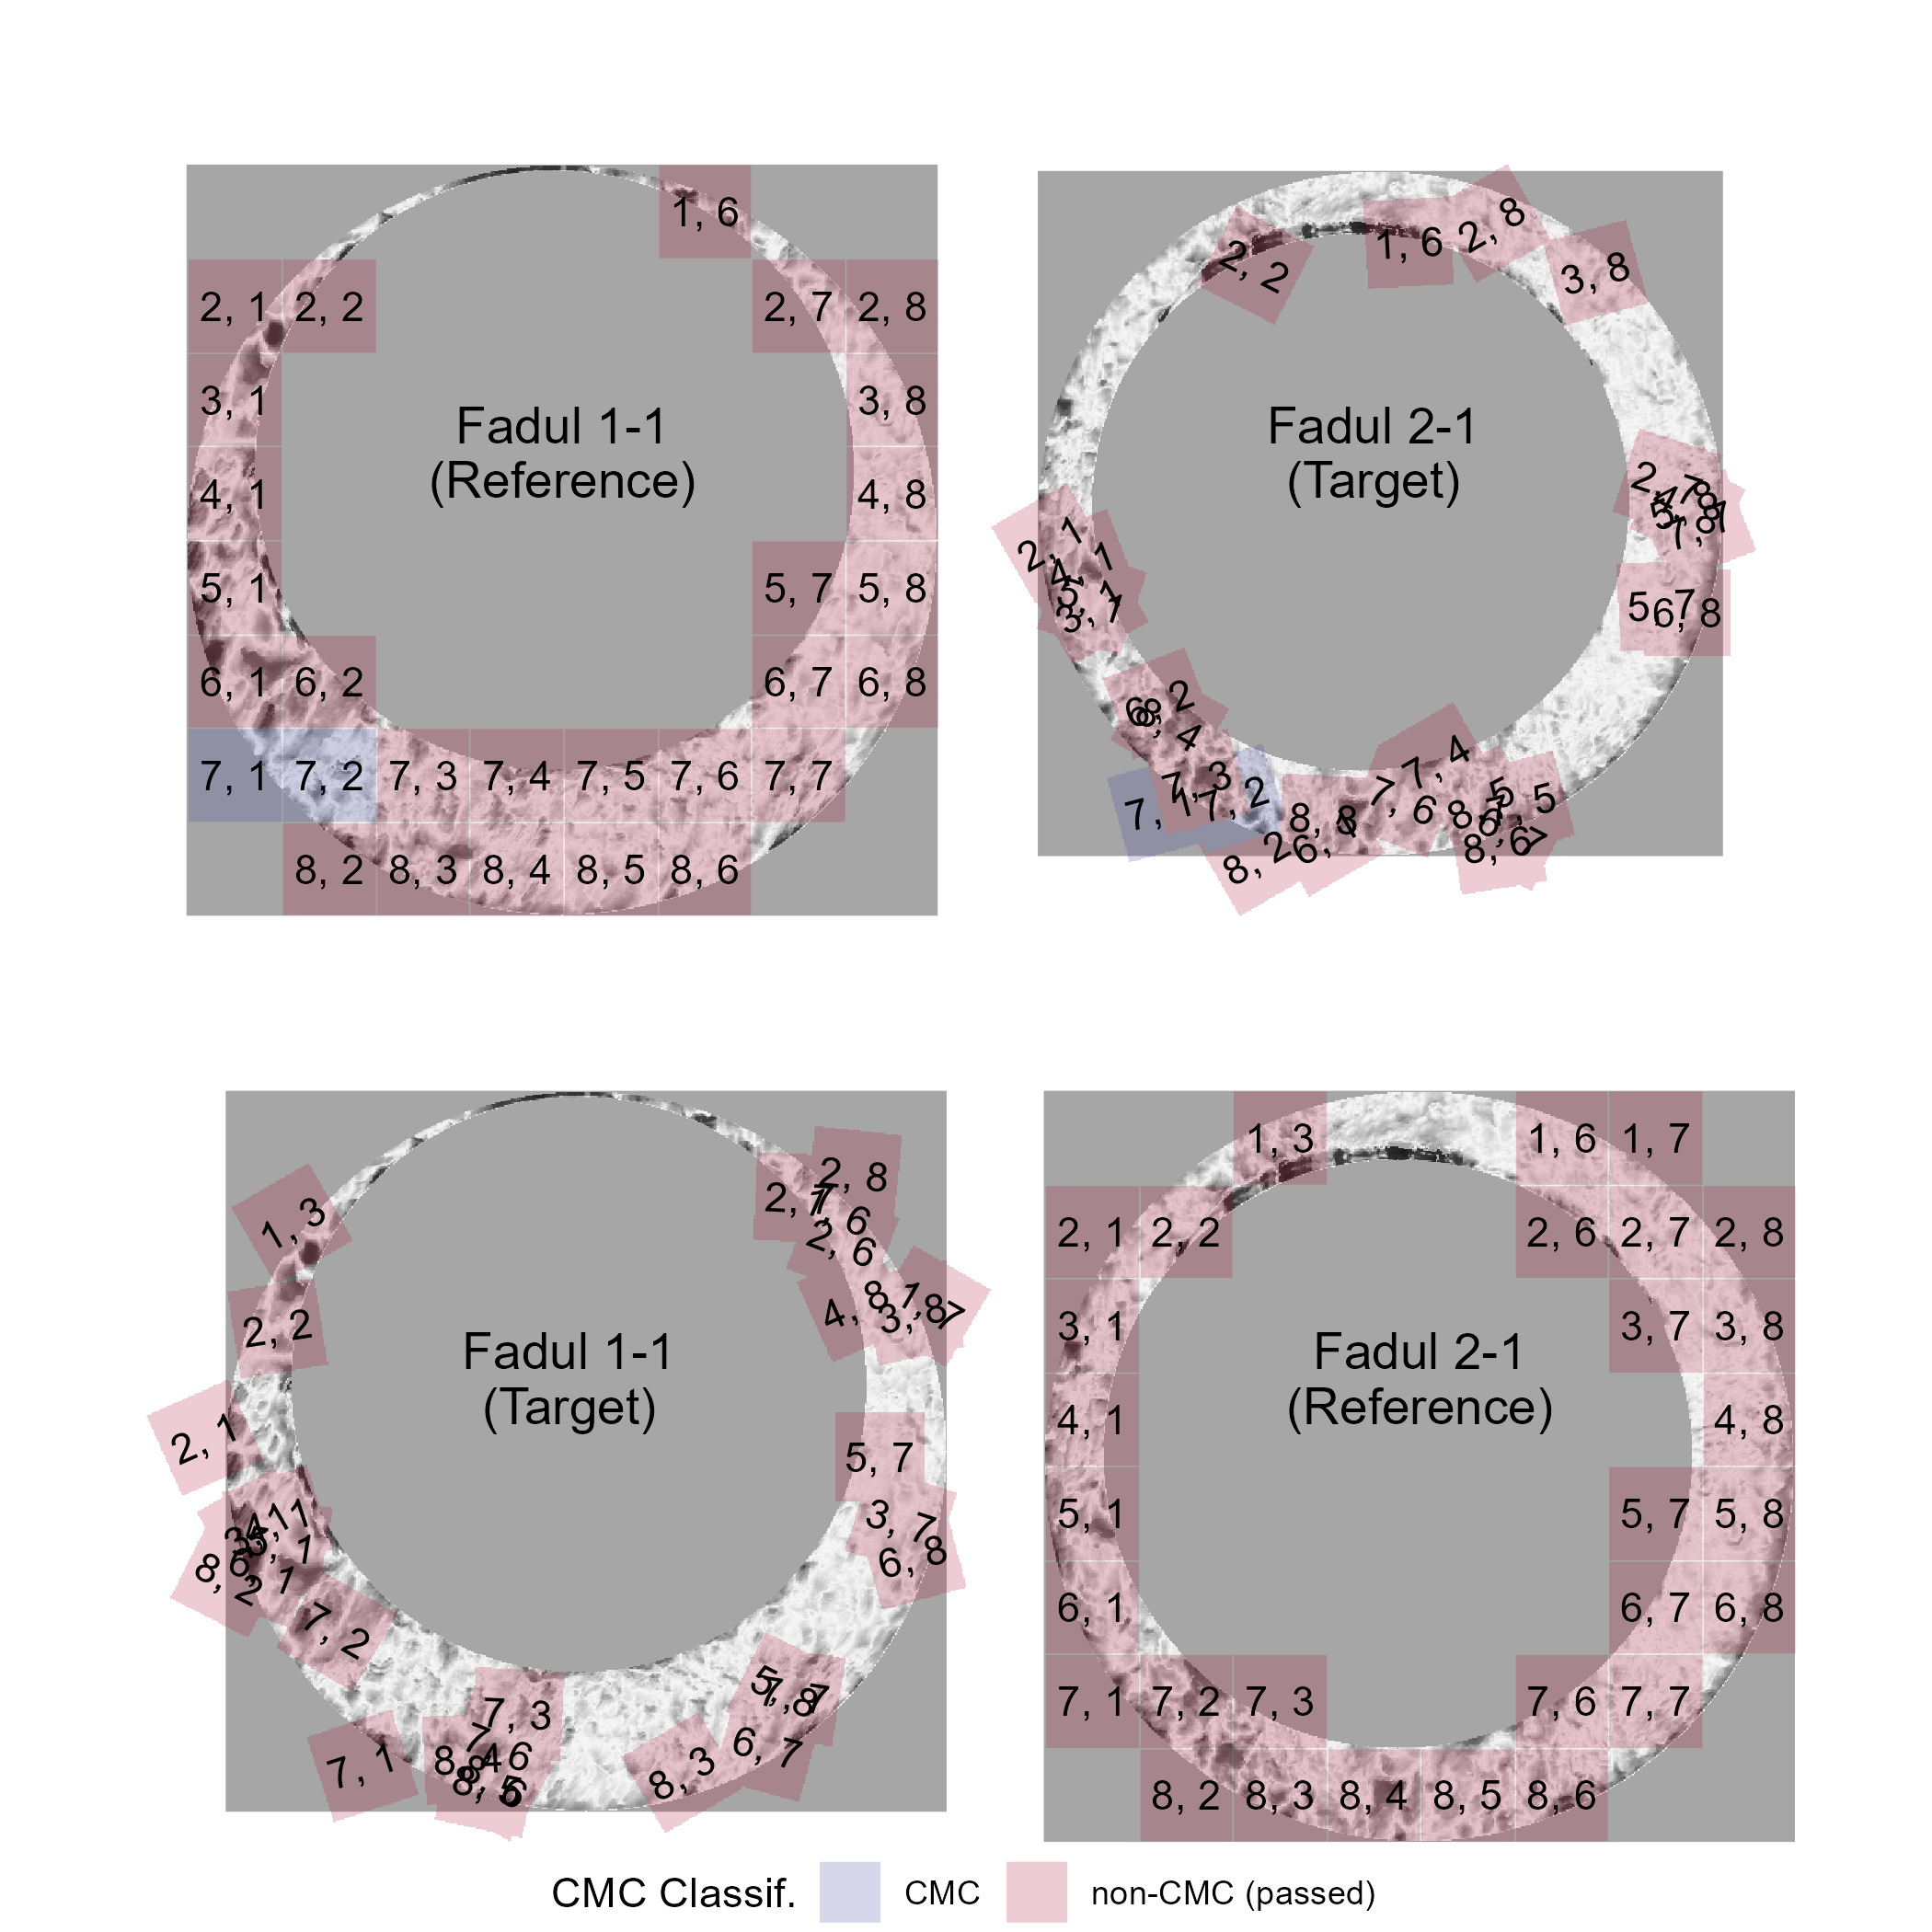
\includegraphics[width=29.17in]{figures/knmOriginalMethod} 

}

\caption{Applying both decision rules to the comparison between the non-match pair Fadul 1-1 and Fadul 2-1 results in 2 CMCs under the original decision rule (shown above) and 0 CMCs under the High CMC decision rule (not shown). The seemingly random behavior of the red cells exemplifies the assumption that cells in a non-match comparison do not exhibit an observable pattern. Random chance should be the prevailing factor in classifying non-match cells as CMCs.}\label{fig:knmCMCPlot}
\end{figure}

\hypertarget{discussion}{%
\section{Discussion}\label{discussion}}

\hypertarget{ambiguities}{%
\subsection{Ambiguity in algorithmic descriptions}\label{ambiguities}}

During the implementation process we encountered ambiguous descriptions of the various CMC pipelines.
We include the pre-processing and cell-based comparison procedures in the description of CMC methodology to emphasize how sensitive the final results are to decisions made in these first two steps.
The pre-processing and cell-based comparison procedures are discussed only briefly, if at all, in \citet{song_3d_2014}, \citet{tong_fired_2014}, \citet{tong_improved_2015}, or \citet{chen_convergence_2017}.
However, the results reported often indicate a sensitivity to these procedures.
Ambiguities range from minor implicit parameter choices (e.g., the convergence criteria for the robust Gaussian regression filter \citep{brinkman_bodschwinna_2003}) to procedures that are fundamental to feature calculation (e.g., how the cross-correlation is calculated).
We bring up these ambiguities to demonstrate the difficulties that we faced when translating the conceptual description of the CMC pipeline into an actual pipeline.
While many of these choices are unlikely to affect the results dramatically, we believe that any amount of variability that exists solely because of uncertainty in how the method was intended to be implemented is both unnecessary and dangerous in this application.

The only solution to such ambiguity is to enumerate, implement, and pare-down the possible choices that could have been made to arrive to published results.
Unsurprisingly, this process takes a considerable amount of time and resources that would be better spent furthering the state of the field.
During the creation of the cmcR package, the process of re-implementing the comparison and decision steps of the pipeline was fairly straightforward.
Emulating the pre-processing procedures used, on the other hand, took months of trial and error.
Even after this effort, we still have no assurances that our implementation would match the results of the original implementation if applied to other data sets.

In the next section, we describe the process of resolving these ambiguities in the CMC pipeline descriptions.
In doing so, we abstract a set of principles by which pipelines and results can be rendered both computationally reproducible and more thoroughly understood.

\hypertarget{investigation}{%
\subsection{CMC pattern matching pipeline}\label{investigation}}

As described in the \protect\hyperlink{initialData}{initial data} section, the set of cartridge case scans from \citet{fadul_empirical_2011} is commonly used to compare the performance of various classification methods \citep{song_3d_2014, tong_improved_2015, chen_convergence_2017}.
This set consists of 40 cartridge cases and 780 total comparisons: 63 known match comparisons and 717 known non-match comparisons.
Scans of each breech face impression were taken with a Nanofocus Confocal Light Microscope at 10 fold magnification for a nominal lateral resolution of 3.125 microns per pixel and published to the NBTRD \citep{nbtrd}.
We also use the \citet{weller_2012} data set of 95 cartridge cases for comparison.
For the \citet{weller_2012} dataset, we manually isolated the breech face impression regions using the FiX3P software (accessible here: \url{https://github.com/talenfisher/fix3p}).
We compare results from the cmcR package to published results using processed scans available through the Iowa State University DataShare repository \citep{cartridgeCaseDataSet}.
Our goal is to show that results obtained from cmcR are similar, at least qualitatively, to previously published results.
However, justification for any differences will ultimately involve educated guesses due to the closed-source nature of the original implementations.

For each cartridge case pair, we calculate CMC counts under both the original and High CMC decision rules.
In practice, we classify a cartridge case pair as ``matching'' if its CMC count surpasses some threshold; 6 CMCs being the generally accepted threshold in many papers \citep{tong_improved_2015, song_estimating_2018, song_proposed_2013}.
However, this threshold has been shown to not generalize well to all proposed methods and cartridge case data sets \citep{chen_convergence_2017}.
We instead use an optimization criterion to select parameters.
In doing so, we will demonstrate the sensitivity of the pipeline to parameter choice.
Additionally, we introduce a set of principles designed to reduce the need for brute-force searches across parameter settings when re-implementing algorithms without accompanying code.
Adherence to these principles yields not only computationally reproducible results, but also improves a reader's understanding of a proposed pipeline.

\hypertarget{processing-condition-sensitivity}{%
\subsection{Processing condition sensitivity}\label{processing-condition-sensitivity}}

Choosing threshold values \(T_x, T_y, T_\theta, T_{\text{CCF}}\) for translation, rotation, and maximum cross-correlation is crucial in declaring a particular cell-region pair ``congruent.''
However, many combinations of these thresholds yield perfect separation between the matching and non-matching CMC count distributions.
Therefore, choosing parameters based on maximizing classification accuracy does not lead to an obvious, single set of parameters.
We instead consider the ratio of between- and within-group variability to measure separation between match and non-match CMC counts.

Let C\(_{ij}\) denote the CMC count assigned to the \(j\)th cartridge case pair, \(j = 1,...,n_i\) from the \(i\)th group, \(i = 1,2\) representing matches and non-matches, respectively.
For each set of thresholds we calculate the \textbf{Variance Ratio} \(r\) as:
\[
r = r\left(T_x, T_y, T_\theta, T_{\text{CCF}}\right) = \frac{\sum_{i=1}^2 \left(\overline{C}_{i.} - \overline{C}_{..}\right)^2}{\sum_{i=1}^2 \frac{1}{n_i - 1}\sum_{j=1}^{n_i} \left(C_{ij} - \overline{C}_{i.}\right)^2},
\]
where \(\overline{C}_{i.}\) denotes the within-group CMC count average and \(\overline{C}_{..}\) denotes the grand CMC count average.
Greater separation between and less variability within the match and non-match CMC count distributions yields larger \(r\) values.

For example, Figure \ref{fig:decisionRuleSensitivity-comparison} shows results for the original decision rule and the High CMC decision rule for parameters \(T_x = 20 = T_y\) pixels, \(T_{\text{CCF}} = 0.5\), and \(T_{\theta} = 6\).
Despite both decision rules resulting in separation between the matching and non-matching CMC count distributions, the High CMC decision rule yields greater separation as evidenced by the larger \(r\) value.

\begin{figure}[htbp]

{\centering 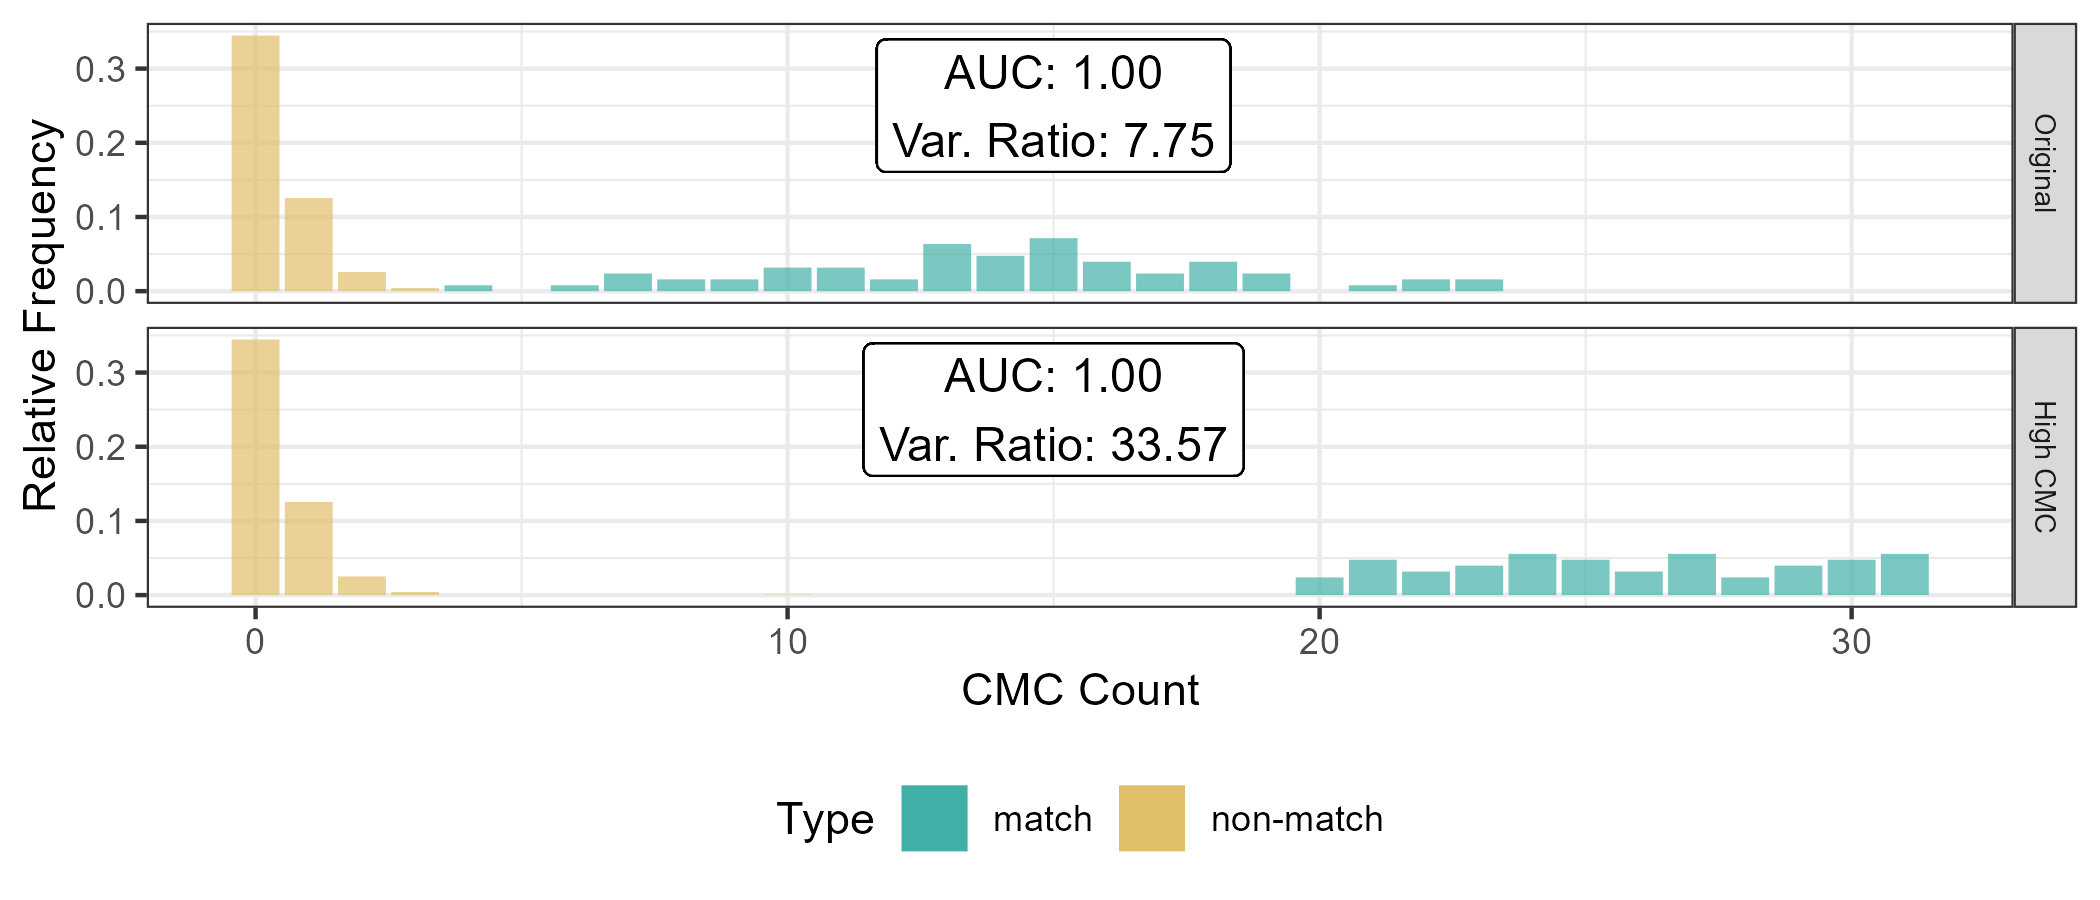
\includegraphics[width=29.17in]{figures/cmcDistributionExample} 

}

\caption{CMC count relative frequencies under the original decision rule and the High CMC decision rule for $T_{\Delta x} = 20 = T_{\Delta y}$ pixels, $T_{\text{CCF}} = 0.5$, and $T_{\theta} = 6$ degrees. An AUC $= 1$ corresponds to perfect separation of the match and non-match CMC count distributions. We can see that, for this set of processing parameters, the High CMC decision rule yields higher CMC counts for known matches that the original decision rule while known non-matches have the same distribution under both methods.}\label{fig:decisionRuleSensitivity-comparison}
\end{figure}

To explore the pipeline's sensitivity, we consider five dimensions that have a demonstrable impact on CMC counts:

\begin{itemize}
\item
  the decision rule (original or High CMC) used,
\item
  whether the global trend is removed during pre-processing, and
\item
  choice of congruency thresholds: translation \(T_x, T_y\), rotation \(T_\theta\), and cross-correlation \(T_{\text{CCF}}\).
\end{itemize}

Choosing a single parameter setting that results in perfect identification is not enough to generally understand the algorithm.
Instead, we use the variance ratio \(r\) to identify promising ranges of parameters.
Figure \ref{fig:cmc-sensitivityScatter} shows the value of the variance ratio under different parameter settings.
We see that the High CMC decision rule yields better separation than the original decision rule under any parameter setting.
The largest variance ratio values are achieved for thresholds \(T_x, T_y \in [10,20]\), \(T_\theta = 6\), and \(T_{\text{CCF}} \in [0.4,0.5]\).
Interestingly, considering Table \ref{tab:thresholdTable-latex}, only the parameters used in \citet{song_estimating_2018} fall into these ranges.

\begin{figure}[htbp]

{\centering 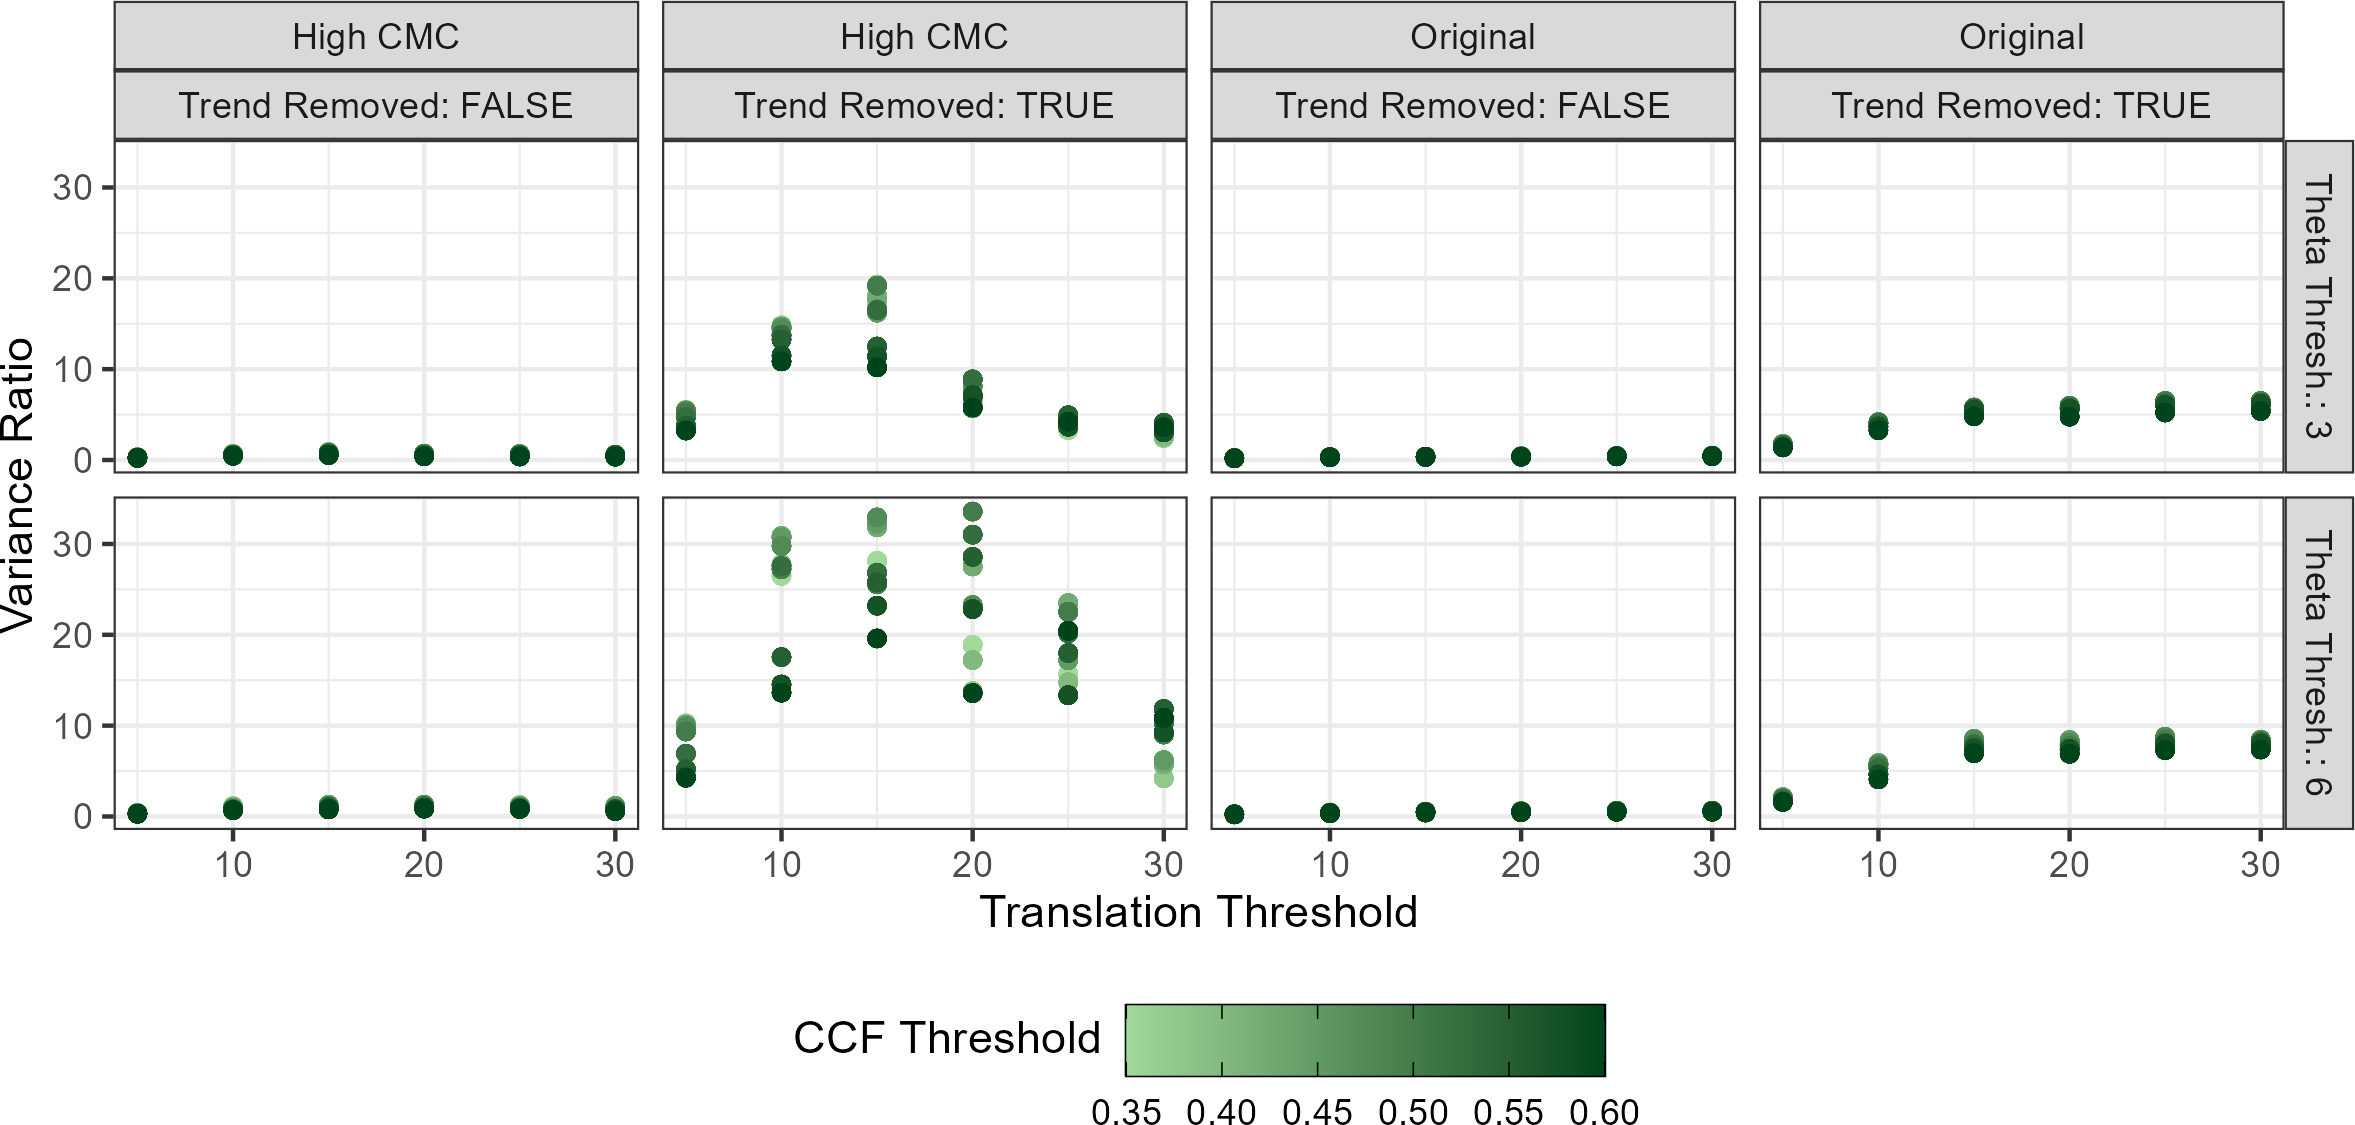
\includegraphics[width=33.33in]{figures/varianceRatioPlt} 

}

\caption{Variance ratio values are plotted for different parameter settings. High variance ratios are indicative of a a good separation between CMC counts for known matching pairs and known-non matching pairs. The High CMC decision rule generally performs better than the original decision rule. Removing the trend during pre-processing has a major impact on the effectiveness of the CMC pipeline. In this setting, translation thresholds $T_x, T_y \in [15,20]$, a rotation threshold $T_\theta = 6$, and a CCF threshold $T_{\text{CCF}} \in [0.4,0.5]$ lead to a separation of results. }\label{fig:cmc-sensitivityScatter}
\end{figure}

As shown in Figure \ref{fig:cmc-sensitivityScatter}, de-trending breech-scans in the pre-processing stage emerges as a critical step to achieve good algorithmic results.
This step is not explicitly mentioned in the written-word descriptions of the algorithm in \citet{song_proposed_2013}, \citet{tong_fired_2014}, \citet{tong_improved_2015}, \citet{chen_convergence_2017}, or \citet{song_estimating_2018}, though it appears from their examples that it was used in the process.
Figure \ref{fig:cmc-sensitivityScatter} also illustrates how breaking a pipeline up into modularized steps eases experimentation.
We will expand upon this idea in the next section.

We compare the best results from cmcR to results presented in previous papers.
In particular, we have calculated variance ratio statistics shown in Figure \ref{fig:cmc-varRatioComparison} based on CMC counts reported in \citet{song_proposed_2013}, \citet{tong_fired_2014}, \citet{tong_improved_2015}, \citet{chen_convergence_2017}, and \citet{song_estimating_2018}.
The last row in each facet shows the variance ratio values obtained from cmcR.
We see that the implementation provided in cmcR yields comparable results to previous CMC papers.

\begin{figure}[htbp]

{\centering 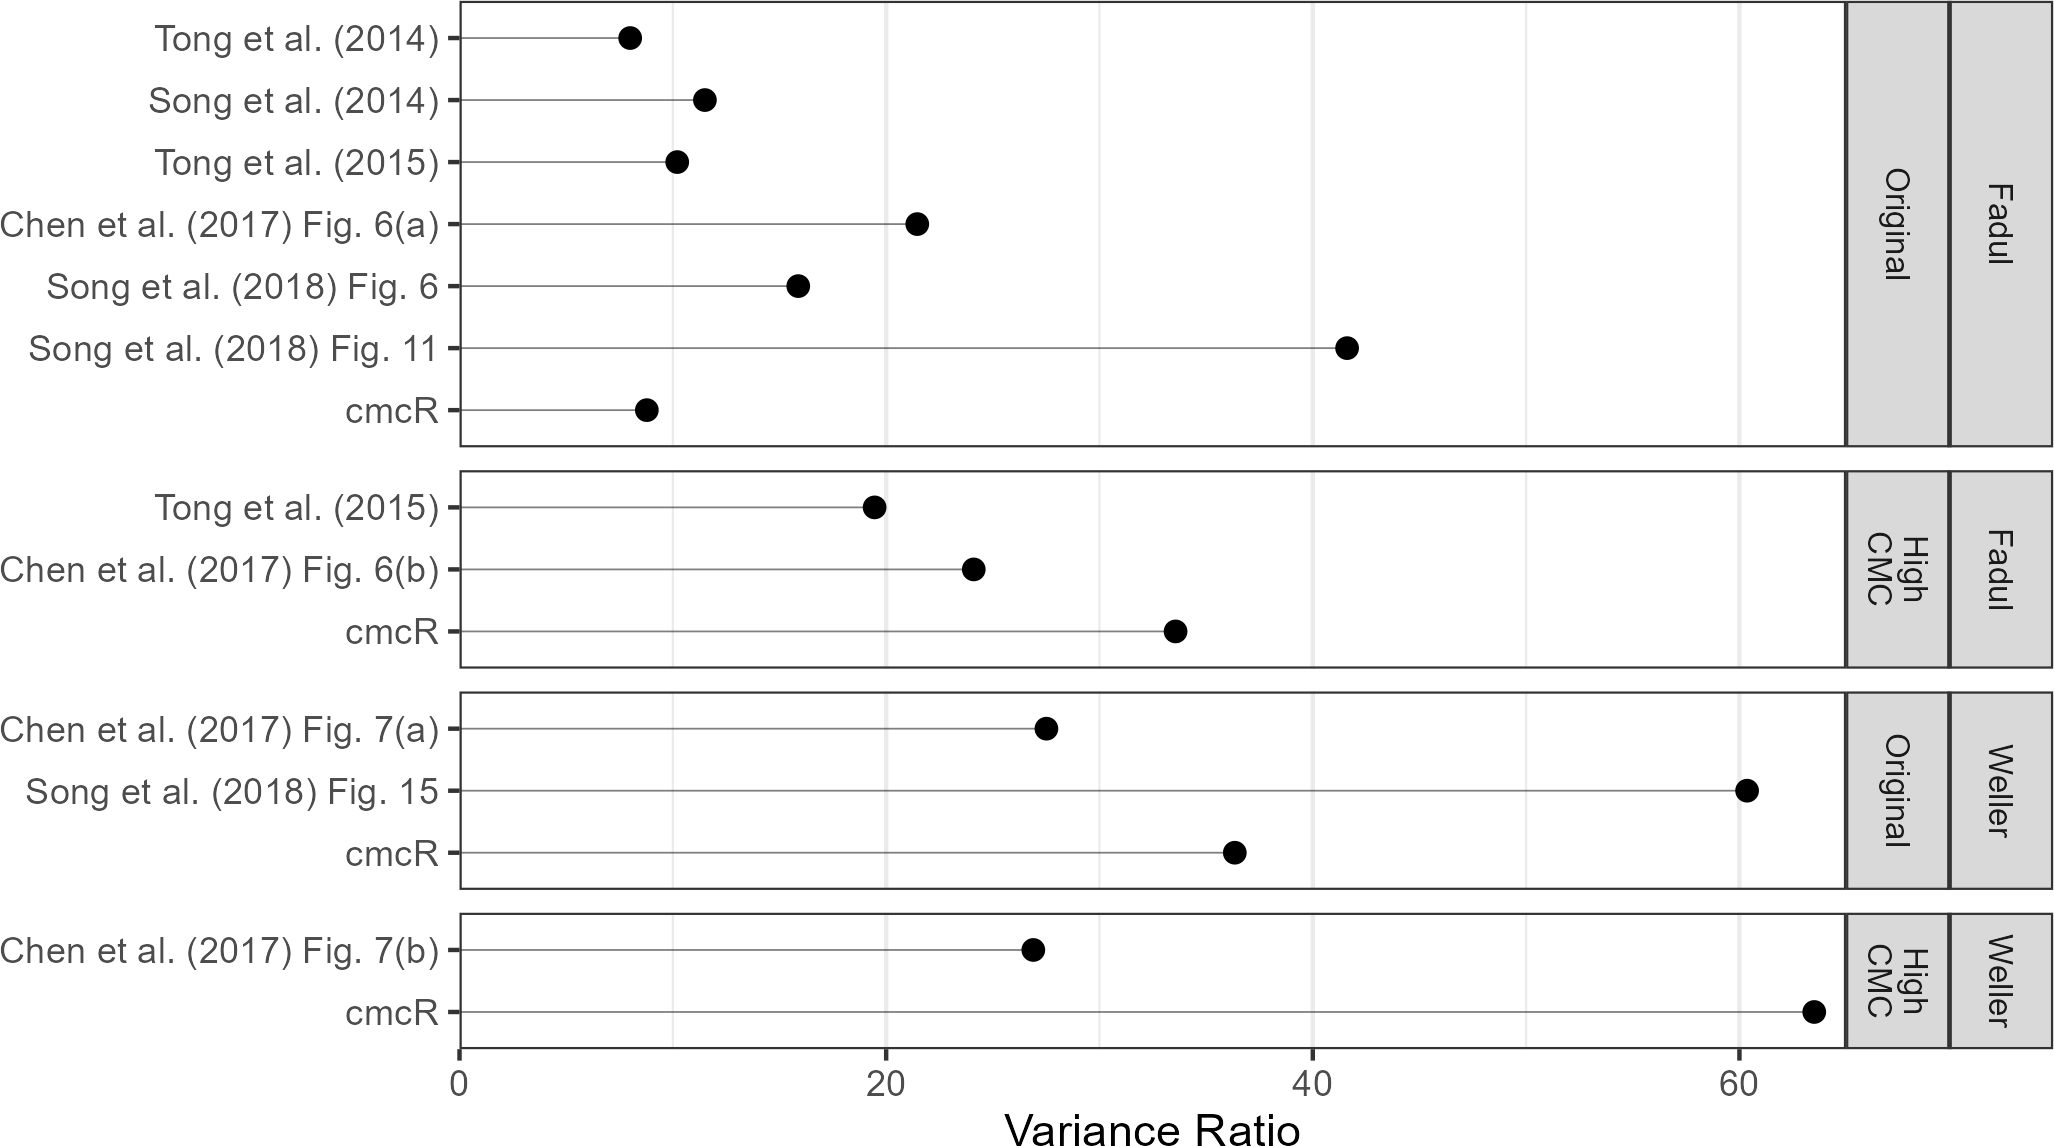
\includegraphics[width=29.17in]{figures/varianceRatio_paperComparisons} 

}

\caption{Variance ratios based on results reported in various CMC papers. The High CMC decision rule tends to outperform the original decision rule. However, it should be emphasized that each paper uses very different processing and parameter settings meaning the results are difficult to compare. The values labeled "cmcR" show the largest variance ratio values for the original and High CMC decision rules based on a limited grid search. These results indicate that the CMC pipeline implementation provided in cmcR yields comparable results to previous CMC papers.}\label{fig:cmc-varRatioComparison}
\end{figure}

\hypertarget{conclusion}{%
\section{Conclusion}\label{conclusion}}

Reproducibility is an indispensable component of scientific validity \citep{goodman_what_2016}.
In this paper, we demonstrate at least three ways reproducibility can go awry: ambiguity in procedural implementation, missing or incomplete data, and missing or incomplete code.
In forensics, many matching algorithms are commonly presented in the form of conceptual descriptions with accompanying results.
There is sound reasoning to this; conceptual descriptions are more easily understood by humans compared to computer code.
However, using the CMC pipelines as an example we have observed the gaps that can exist when translating a conceptual description of an algorithm to a genuine implementation.
This is largely due to the fact that conceptual descriptions rarely detail implicit parameter choices required to run an algorithm.
Consequently, there are multiple choices that are compatible with the description of an algorithm in a publication.
This is dangerous in a forensics context because if many parameter settings are valid but only a narrow range lead to the same conclusion, it is entirely possible that witnesses for the prosecution and defense comef to different conclusions.
In order to prevent such misunderstandings, it is not enough to have guidelines for parameter settings and/or a sensitivity study -- it is also necessary to standardize the specific computer code.
The parameter values are only useful within the context of a single software package or pipeline.

These principles of open, accessible, interoperable code are also critical for a fair (in the legal sense) justice system: the defense has access to the code to understand the evidence against them, lawyers and examiners can assess the utility of the analysis method, and judges can determine whether a method is admissible in court.
Transparent and intuitive open-source algorithms, such as cmcR, should be considered the gold standard in allowing the forensic science community to validate a pipeline.

Our contribution to the CMC literature is the open-source implementation, which fills the gaps in the human-friendly descriptions in the original papers.
In addition, because we have structured the cmcR implementation as a modular pipeline, it is easier to improve upon the CMC method and document the effects of specific changes to the algorithm compared to previous versions.
The modularization creates an explicit framework to assess the utility and effectiveness of each piece of the algorithm, and allows us to independently manipulate each step while monitoring the downstream impact on the results.
Additionally, it allows future collaborators to improve on pieces of the pipeline, adding new options and improving the method without having to re-invent the wheel.
Indeed, re-implementing steps of the pipeline is at best a useful academic exercise and at worst a waste of time and resources that could be spent actually improving the pipeline.
Even after many months of trial and error, although we have succeeded in obtaining qualitatively similar results on two data sets, it is difficult to know whether our implementation will behave the same as previous implementations on external data sets.
Generalizability is an important assessment for any computational algorithm \citep{vanderplasComparisonThreeSimilarity2020}.

Our application is far from unique: some journals have adopted policies encouraging or requiring that authors provide code and data sufficient to reproduce the statistical analyses, with the goal of building a ``culture of reproducibility'' in their respective fields \citep{peng_reproducible_2009, peng_reproducible_2011, stodden_toward_2013}.
Peer-review and scientific progress in the truest sense requires that \emph{all} pre-processed data, code, and results be made openly available \citep{kwongAlgorithmSaysYou2017, desaiTrustVerifyGuide2017}.
Our experience with the CMC algorithm suggests that these standards should be adopted by the forensic science community, leveraging open-source ecosystems like R and software sharing platforms such as Github.
We firmly believe that the forensic community should not go only halfway, trading a subjective, human black box for objective, proprietary algorithms that are similarly opaque and unauditable.
Open, fully reproducible packages like cmcR allow research groups to make incremental changes, compare different approaches, and accelerate the pace of research and development.

\hypertarget{acknowledgement}{%
\section{Acknowledgement}\label{acknowledgement}}

This work was partially funded by the Center for Statistics and Applications in Forensic Evidence (CSAFE) through Cooperative Agreement 70NANB20H019 between NIST and Iowa State University, which includes activities carried out at Carnegie Mellon University, Duke University, University of California Irvine, University of Virginia, West Virginia University, University of Pennsylvania, Swarthmore College and University of Nebraska, Lincoln.

We greatly appreciate the constructive feedback from the two anonymous reviewers.
Special thanks also to all the developers and open-source contributors of R, knitr \citep{knitr1, knitr2}, rticles \citep{rticles}, and the tidyverse \citep{tidyverse}, without whom this project would not have been possible.

\hypertarget{computational-details}{%
\section{Computational details}\label{computational-details}}

\begin{verbatim}
#> R version 4.2.2 (2022-10-31 ucrt)
#> Platform: x86_64-w64-mingw32/x64 (64-bit)
#> Running under: Windows 10 x64 (build 22621)
#> 
#> Matrix products: default
#> 
#> locale:
#> [1] LC_COLLATE=English_United States.utf8 
#> [2] LC_CTYPE=English_United States.utf8   
#> [3] LC_MONETARY=English_United States.utf8
#> [4] LC_NUMERIC=C                          
#> [5] LC_TIME=English_United States.utf8    
#> 
#> attached base packages:
#> [1] stats     graphics  grDevices datasets  utils     methods  
#> [7] base     
#> 
#> other attached packages:
#>  [1] patchwork_1.1.2 rgl_1.0.1       x3ptools_0.0.3  lubridate_1.9.2
#>  [5] forcats_1.0.0   stringr_1.5.0   purrr_1.0.1     readr_2.1.4    
#>  [9] tidyr_1.3.0     tibble_3.2.0    tidyverse_2.0.0 cmcR_0.1.11    
#> [13] dplyr_1.1.0     magrittr_2.0.3  ggplot2_3.4.1  
#> 
#> loaded via a namespace (and not attached):
#>  [1] httr_1.4.5         jsonlite_1.8.4     viridisLite_0.4.0 
#>  [4] splines_4.2.2      assertthat_0.2.1   yulab.utils_0.0.6 
#>  [7] renv_0.15.5        tiff_0.1-11        yaml_2.3.5        
#> [10] pillar_1.8.1       lattice_0.20-45    quantreg_5.94     
#> [13] glue_1.6.2         digest_0.6.29      rvest_1.0.3       
#> [16] colorspace_2.0-3   readbitmap_0.1.5   cowplot_1.1.1     
#> [19] htmltools_0.5.4    Matrix_1.5-3       ggnewscale_0.4.8  
#> [22] pkgconfig_2.0.3    SparseM_1.81       bookdown_0.26     
#> [25] scales_1.2.0       webshot_0.5.4      ggplotify_0.1.0   
#> [28] svglite_2.1.1      jpeg_0.1-10        tzdb_0.3.0        
#> [31] pracma_2.4.2       MatrixModels_0.5-1 timechange_0.2.0  
#> [34] farver_2.1.0       generics_0.1.2     ellipsis_0.3.2    
#> [37] withr_2.5.0        cli_3.6.0          survival_3.4-0    
#> [40] evaluate_0.15      fansi_1.0.3        MASS_7.3-55       
#> [43] imager_0.42.18     xml2_1.3.3         textshaping_0.3.6 
#> [46] tools_4.2.2        hms_1.1.2          bmp_0.3           
#> [49] lifecycle_1.0.3    munsell_0.5.0      kableExtra_1.3.4  
#> [52] compiler_4.2.2     gridGraphics_0.5-1 systemfonts_1.0.4 
#> [55] rlang_1.0.6        grid_4.2.2         rstudioapi_0.14   
#> [58] htmlwidgets_1.6.1  igraph_1.4.1       labeling_0.4.2    
#> [61] base64enc_0.1-3    rmarkdown_2.14     gtable_0.3.0      
#> [64] codetools_0.2-18   R6_2.5.1           gridExtra_2.3     
#> [67] zoo_1.8-11         knitr_1.39         fastmap_1.1.0     
#> [70] utf8_1.2.2         ragg_1.2.5         stringi_1.7.6     
#> [73] Rcpp_1.0.10        vctrs_0.5.2        png_0.1-8         
#> [76] tidyselect_1.2.0   xfun_0.31
\end{verbatim}

\hypertarget{diagnostic-tools-for-cartridge-case-comparison-algorithms}{%
\chapter{Diagnostic Tools for Cartridge Case Comparison Algorithms}\label{diagnostic-tools-for-cartridge-case-comparison-algorithms}}

\hypertarget{abstract-1}{%
\section*{Abstract}\label{abstract-1}}
\addcontentsline{toc}{section}{Abstract}

Diagnostics are useful for explaining the behavior of a complex model or algorithm.
In this paper, we introduce a suite of visual and interactive diagnostic tools to assess algorithms that automatically compare forensic cartridge case evidence.
These tools are useful to both forensic researchers and practitioners:
Researchers can analyze and correct the (mis)behavior of the algorithm forensic practitioners can more easily understand and explain the algorithm.
First, we develop a collection of tools to diagnose each step of a cartridge case comparison algorithm in the \texttt{impression} R package.
We then implement these visual diagnostics in an interactive web application called \texttt{cartridgeInvestigatR} to provide greater flexibility to the user.

\hypertarget{introduction}{%
\section{Introduction}\label{introduction}}

Start of paper.

\hypertarget{automatic-matching-of-cartridge-case-impressions}{%
\chapter{Automatic Matching of Cartridge Case Impressions}\label{automatic-matching-of-cartridge-case-impressions}}

\hypertarget{abstract-2}{%
\section*{Abstract}\label{abstract-2}}
\addcontentsline{toc}{section}{Abstract}

Forensic examinations attempt to solve the binary classification problem of whether two pieces of evidence originated from the same source.
For example, a cartridge case found at a crime scene may be compared to a cartridge case fired from a suspect's firearm.
Forensic examiners traditionally rely on high-powered comparison microscopes, case facts, and their own experience to arrive at a source conclusion.
Recently, algorithms that provide an automatic and objective measure of similarity of the evidence have become more prevalent.
We introduce the Automatic Cartridge Evidence Scoring (ACES) algorithm that encompasses preprocessing, feature extraction, and similarity scoring.
Our primary contribution is a set of features used to classify whether two cartridge cases were fired from the same firearm.
We use a train/test split on a data set of 510 cartridge case scans to fit and validate random forest, logistic regression, and Classification and Regression Tree (CART) models.
We demonstrate that these models are more accurate than predominant algorithms on our data set.

\hypertarget{introduction-1}{%
\section{Introduction}\label{introduction-1}}

Start of paper.

\renewcommand\bibname{\centerline{REFERENCES}}
\unappendixtitle
\newpage
\phantomsection
\addcontentsline{toc}{chapter}{REFERENCES}
\bibliography{resources/litReviewBib.bib}


\end{document}
